% arara: clean: {files: [thesis.aux, thesis.idx, thesis.ilg, thesis.ind, thesis.log, thesis.bbl, thesis.bcf, thesis.ist, thesis.blg, thesis.run.xml, thesis.lol, thesis.out, thesis.toc, texput.log]}
% arara: lualatex: { shell : yes , action: batchmode, draft: yes}
% arara: biber
% arara: lualatex: { shell : yes , action: batchmode, draft: yes}
% arara: lualatex: { shell : yes , action: batchmode}

\documentclass[a4paper,11pt]{kth-mag}
\DeclareMathSizes{10.95}{12}{9}{7}
%\DisemulatePackage{setspace}
%\usepackage[onehalfspacing]{setspace}

% Math and code packages
\usepackage{amsmath}   % all things math
\usepackage{amssymb}   % additional math symbols
\usepackage{xfrac}     % nice fractions in body of text
\usepackage{siunitx}   % typesets numbers with units
\usepackage{mathtools} % extensions for amsmath
\usepackage[chapter]{minted}    % advanced code examples

% Tables
\usepackage{booktabs} % professionally looking tables
\usepackage{tabulary} % whole page tables

% Caption and split floats
\usepackage{caption}    % customizable captions
\usepackage{subcaption} % nice subfigures and subtables

% Bibliographies
\usepackage[
  backend=biber,
  style=numeric
]{biblatex} % modern bibliographies
\addbibresource{thesis.bib}
\usepackage{csquotes}

% PDF Metadata
\usepackage{hyperref} % enables PDF hyperlinks

% Fonts, typography and languages
\usepackage{fontspec}     % all things fonts
\defaultfontfeatures{Ligatures=TeX}
\setmainfont{FiraSans-Book.otf}[
  BoldFont = FiraSans-SemiBold.otf,
  ItalicFont = FiraSans-Italic.otf,
  BoldItalicFont = FiraSans-SemiBoldItalic.otf]
\setsansfont{FiraSans-Regular.otf}[Scale=MatchLowercase]
\setmonofont{FiraMono-Regular.otf}[Scale=MatchLowercase]
\usepackage{unicode-math} % use custom fonts for math
\setmathfont{Asana-Math.otf}
\usepackage{microtype}	  % advanced typesetting
\DisableLigatures{family=tt*}
\usepackage[main=english, swedish]{babel} % language-specific conventions

\clubpenalty=10000
\widowpenalty=10000
\displaywidowpenalty = 10000

% Graphics
\usepackage{graphicx} % all things graphics
\usepackage{pgfplots} % complex graphs
\usepgfplotslibrary{dateplot}
\usepackage{pgfplotstable}
\usepgfplotslibrary{fillbetween}
\usetikzlibrary{pgfplots.fillbetween}
\pgfplotsset{
  compat=1.11, % avoid running in backwards compatibility mode
  width=\textwidth,
  tick label style = {font=\sffamily},
  every axis label = {font=\sffamily},
  legend style = {font=\sffamily},
  label style = {font=\sffamily},
  separate axis lines,
  y axis line style={draw opacity=0},
  x axis line style={gray},
  axis x line*=bottom,
  axis y line*=left,
  major tick length=0pt,
  grid=both,
  y grid style={dashed},
  legend pos=north west,
  tick label style={/pgf/number format/assume math mode=true},
}
\definecolor{set11}{RGB}{228,  26,  28}
\definecolor{set12}{RGB}{ 55, 126, 184}
\definecolor{set13}{RGB}{ 77, 175,  74}
\definecolor{set14}{RGB}{152,  78, 163}
\definecolor{set15}{RGB}{255, 127,   0}
\definecolor{set16}{RGB}{255, 255,  51}
\definecolor{set17}{RGB}{166,  86,  40}
\definecolor{set18}{RGB}{247, 129, 191}
\definecolor{set19}{RGB}{153, 153, 153}

\definecolor{set11_light}{RGB}{251, 180, 174}
\definecolor{set12_light}{RGB}{179, 205, 227}
\definecolor{set13_light}{RGB}{204, 235, 197}
\definecolor{set14_light}{RGB}{222, 203, 228}
\definecolor{set15_light}{RGB}{254, 217, 166}
\definecolor{set16_light}{RGB}{255, 255, 204}
\definecolor{set17_light}{RGB}{229, 216, 189}
\definecolor{set18_light}{RGB}{253, 218, 236}
\definecolor{set19_light}{RGB}{242, 242, 242}

% \definecolor{set11}{cmyk}{.1 ,.9 ,.8 ,.0 }
% \definecolor{set12}{cmyk}{.8 ,.3 ,.0 ,.0 }
% \definecolor{set13}{cmyk}{.7 ,.0 ,.8 ,.0 }
% \definecolor{set14}{cmyk}{.4 ,.65,.0 ,.0 }
% \definecolor{set15}{cmyk}{.0 ,.5 ,1.0,.0 }
% \definecolor{set16}{cmyk}{.0 ,.0 ,.8 ,.0 }
% \definecolor{set17}{cmyk}{.35,.6 ,.8 ,.0 }
% \definecolor{set18}{cmyk}{.0 ,.5 ,.0 ,.0 }
% \definecolor{set19}{cmyk}{.0 ,.0 ,.0 ,.4 }
%
% \definecolor{set11_light}{cmyk}{.0 ,.3 ,.2 ,.0 }
% \definecolor{set12_light}{cmyk}{.3 ,.1 ,.0 ,.0 }
% \definecolor{set13_light}{cmyk}{.2 ,.0 ,.2 ,.0 }
% \definecolor{set14_light}{cmyk}{.12 ,.17,.0 ,.0 }
% \definecolor{set15_light}{cmyk}{.0 ,.15 ,.3,.0 }
% \definecolor{set16_light}{cmyk}{.0 ,.0 ,.2 ,.0 }
% \definecolor{set17_light}{cmyk}{.1,.12 ,.2 ,.0 }
% \definecolor{set18_light}{cmyk}{.0 ,.15 ,.0 ,.0 }
% \definecolor{set19_light}{cmyk}{.0 ,.0 ,.0 ,.05 }

\newcommand{\POS}{\mathbf{x}}
\newcommand{\ORIENT}{\mathbf{t}}
\newcommand{\DIFFPOINT}{\mathbf{x} - \mathbf{y}}

\linespread{1.213}

\usepackage{modifications}

\title{GPU Simulation of Rigid Fibers}

\foreigntitle{GPU simulering av stela fibrer}

\author{Eric Wolter}
\date{January 2015}
\blurb{Master's Thesis at School of Engineering Sciences\\Supervisor: Katarina Gustavsson\\Examiner: Michael Hanke}
\trita{TRITA xxx yyyy-nn}

\begin{document}
\frontmatter
\pagestyle{empty}

\maketitle
\selectlanguage{english}
\begin{abstract}
The major objective of this Master's thesis is to accelerate a serial implementation of a numerical algorithm for the simulation of slender fiber dynamics by using Graphical Processing Units (GPU). We focus on rigid fibers sedimenting due to gravity in a free-space Stokes flow. The ability to simulate a large number of fibers in a reasonable computational time on a high-performance parallel platform opens exciting new research opportunities.

The previous serial implementation is rewritten for parallel execution. The algorithm is implemented in single precision using the Compute Unified Device Architecture (CUDA) on NVIDIA GPUs. In addition, we develop an OpenMP version of the parallel implementation to run on multi-core CPUs. Using both implementations, we perform a number of benchmarks to determine the fastest variant of the algorithm. We observe a speedup of $20×$ to $40×$ on the NVIDIA GTX 970 compared to an Intel Core i7 4770. The GPU implementation can simulate up to $2000$ fibers on a desktop computer and it takes only in the order of $8$ seconds to advance one time step.

Furthermore, we have performed a number of simulations of known experiments for sedimenting fibers to validate the algorithm and to explore the numerical precision of the results. The results show an excellent agreement with results from prior experiments in the field.
\end{abstract}
\clearpage

\begin{foreignabstract}{swedish}
Huvudsyftet med denna masteruppsats är att accelerera en seriell implementation av en numerisk algoritm för simulering av tunnfiberdynamik med hjälp av grafikprocessorer (GPU:er). Vårt fokus ligger på sedimentering av stela fibrer som en konsekvens av gravitationens påverkan i ett frirums-Stokes-flöde. Att kunna simulera ett stort antal fibrer med en relativt kort beräkningstid på en högpresterande parallellplatform öppnar för nya spännande forskningsmöjligheter. 

Den föregående seriella implementationen var skriven för parallellexekvering. Algoritmen är implementerad i enkelprecision med hjälp av Compute Unified Device Architecture (CUDA) på NVIDIA-GPU:er. Vi utvecklar dessutom en OpenMP-version av parallellimplementationen för flerkärnsprocessorer. Genom att använda båda implementationerna utför vi ett antal prestandatester för att hitta den snabbaste varianten av algoritmen. Vi observerar en ökning från $20×$ till $40×$ på NVIDIA GTX 970 jämfört med en Intel Core i7 4770. GPU-implementationen kan simulera upp till $2000$ fibrer på en skrivbordsdator, och det tar endast i ordningen $8$ sekunder att avancera ett tidssteg. 

Vi har dessutom utfört ett antal simuleringar av redan kända experiment för sedimentering av fibrer för att bekräfta att algoritmen är korrekt, samt för att utvärdera resultatens numeriska precision. Resultaten överensstämmer utomordentligt väl med tidigare resultat från experiment i området. 
\end{foreignabstract}
\clearpage

\section*{Acknowledgements}
\clearpage

\tableofcontents*
\clearpage

\listoffigures
\clearpage

\listoftables
\clearpage

\addcontentsline{toc}{chapter}{List of Listings}
\listoflistings
\clearpage

\mainmatter
\pagestyle{newchap}

\chapter{Introduction}

Predicting the physical behavior of particles suspended in fluids is of great interest in a variety of different fields. The ability to accurately model and simulate different categories of particle suspensions allows their properties to be analyzed and optimized for a large number of applications. Examples include medical applications were the delivery and distribution of the active agent has to be modeled, waste management to efficiently extract waste from water and the paper industry which is trying to improve the characteristics of\linebreak their material.

Even in the simplest flow cases, the flow of a particle suspension exhibits very complex and complicated dynamical behavior. The rheological properties of the suspension depend strongly on features such as the concentration of particles, particle shapes and particle interactions. In order to accurately capture the complex dynamics of a suspension using numerical simulations, a large number of particles are required in the simulation. Hence, the ability of the numerical algorithm to efficiently handle a large amount of particles is of\linebreak crucial importance.

The work in this thesis focuses on increasing and optimizing the efficiency of a numerical algorithm for the simulation of sedimenting rigid and slender fibers in a viscous fluid. The fibers are modeled and simulated on a particle-level in a 3D free-space Stokes fluid. The mathematical model is based on a boundary integral formulation and a non-local slender body approximation by\linebreak Tornberg and Gustavsson,~\cite{Tornberg2006}.

\pagebreak
There are many numerical studies of fiber suspension and several different methods have been developed for both rigid and flexible fibers. One approach is the so-called beads-model, where the fibers are modeled as a set of connected spherical beads (e.g.~\cite{Fan1998}\cite{Joung2001}\cite{Skjetne1997}\cite{Yamamoto1995}). The immersed boundary method discretizes the fibers with Lagrangian markers and distributes the force onto a background grid which is then used to modify the fluid flow (e.g.~\cite{Peskin2002}\cite{Stockie1998}). Another approach is based on slender body theory which uses the large aspect ratio of the fibers to simplify the underlying model (e.g.~\cite{Gustavsson2009}\cite{Tornberg2006}\cite{Tornberg2004}). A comprehensive review of the numerical studies of fiber suspension can be found in\linebreak Guazzelli and Hinch,~\cite{Guazzelli2011}.

In this thesis we develop a high performance GPU implementation of the numerical algorithm for simulating fiber suspension. By taking advantage of the massively parallel architecture of modern GPUs many more fibers can be simulated compared to the previous CPU based implementation of the algorithm. The major goal is to easily and efficiently perform simulations on a high-end desktop computer or workstation readily accessible by the researcher. This will allow the researcher to explore the huge problem space and simulate a large number of fibers in a short amount of time. Thus it enhances the capacity to rapidly iterate and discover interesting test cases. These cases can then be used as a starting point for large scale simulations using computing clusters.

The most costly part of the numerical algorithm is to account for the interactions between all fibers in the system. For the calculations we chose the "naive" algorithm, where the interactions between every pair of fibers is computed. The development of such a naive algorithm is easier, more accurate and in some cases more cost effective than an alternative fast summation approach. A fast summation approach, like the fast multipole method, is both complex to implement and introduces a potentially large performance overhead. Therefore it might not result in the desired performance increase compared to the naive algorithm. Our choice of consumer-grade GPU hardware limits the simulation to single precision, thus maintaining the accuracy is very important. By using the naive algorithm on the GPU the goal is to strike a good balance.

This thesis is divided into the three major parts: \emph{Previous Work}, \emph{GPU Implementation} and \emph{Results}. First we introduce the theoretical foundation of the numerical method in Chapter~\ref{cha:theoretical_foundation} and refer to the original paper by Tornberg and Gustavsson,~\cite{Tornberg2006}, for in-depth details. The numerical algorithm and the serial implementation on the CPU developed in the original paper,~\cite{Tornberg2006}, is presented in Chapter~\ref{cha:serial_implementation}. Together these two chapters form the \emph{Previous Work} part of the thesis. Based on this the \emph{GPU Implementation} part follows. Chapter~\ref{cha:gpu_programming} briefly introduces general purpose computing on the GPU. Combining the previous work and GPU computing, we then describe our new parallel implementation of the numerical algorithm on GPUs in Chapter~\ref{cha:parallel_implementation}. This represents the base for the efficiency and the performance improvements and is therefore the core of the thesis. Afterwards, the final \emph{Results} are presented. The benchmarks in Chapter~\ref{cha:benchmarks} illustrate the achieved performance increase of the parallel \emph{GPU Implementation}. Finally, we perform and compare our simulation results to a few known experiments in Chapter~\ref{cha:experiments}.


\chapter{Theoretical foundation}
\label{cha:theoretical_foundation}
The introduction discussed different applications of rigid fiber simulations. It especially stressed the importance of being able to simulate a large number of fibers in order to generate the various patterns found in real world experiments.

In this chapter, we will present the theoretical foundation of the physics and the mathematical model the simulations are based on. This is required to be able to understand the numerical method used throughout the rest of the thesis. However, the model is only presented in a reduced summary, and for more details please refer to Tornberg and Gustavsson~\cite{Tornberg2006}.

\section{Stokes flow}
\label{sec:stokes_flow}

We are interested in modeling the behavior of objects immersed in an incompressible fluid. We restrict ourselves to rigid bodies, which are slowly sedimenting in the fluid due to gravity. In the most general case, the flow can be modeled by the Navier-Stokes equations,
\begin{equation}
  \label{eq:naviar_stokes_equations}
  \begin{aligned}
    \rho\left(\frac{\delta \mathbf{u}}{\delta t} + (\mathbf{u} \cdot \nabla)\mathbf{u}\right) &= -\nabla p + \mu\nabla^2\mathbf{u} + \mathbf{f} \\
    \nabla \cdot \mathbf{u} &= 0 \text{.}
  \end{aligned}
\end{equation}
where $\mathbf{u}(\mathbf{x})$ denotes the velocity field, $p(\mathbf{x})$ the pressure field and $\mathbf{f}(\mathbf{x})$ the force acting on the fluid at the location $\mathbf{x} = (x,y,z) \in \mathbb{R}^3$. The constant $\mu$ is the viscosity of the fluid. Solving these equations is quite challenging due to their time dependence and non-linearity. However, in this work we are only concerned with slowly moving objects and the Reynolds number $Re = \frac{\rho U L}{\mu}$ is assumed to be very small. Given the constraint that $Re \ll 1$, the inertial and acceleration terms in the Navier-Stokes Eqns.~\eqref{eq:naviar_stokes_equations} can be neglected and we arrive at the linear and time independent Stokes equations,
\begin{equation}
  \label{eq:stokes_equations}
  \begin{aligned}
    \nabla p - \mu \Delta \mathbf{u} &= \mathbf{f} \quad &\text{in} \quad \Omega \text{,}\\
    \nabla \cdot \mathbf{u} &= 0 \quad &\text{in} \quad \Omega \text{.}
  \end{aligned}
\end{equation}

In addition to these equations we need two boundary conditions to solve the system. The first boundary condition accounts for the influence on the fluid from the presence of the objects. Hence, we force the fluid velocity at the boundary of the object to be equal to the velocity of the object itself. These no-slip conditions on the surface of the objects are defined as
\begin{equation}
  \label{eq:boundary_condition_surface}
  \mathbf{u} = \mathbf{u}_\Gamma  \quad \text{on} \quad  \Gamma \text{,}
\end{equation}
where $\Gamma$ denotes the union of all object surfaces and $\mathbf{u}_\Gamma$ the corresponding surface velocity, thus constraining the fluid to have zero velocity relative to the object surfaces.

The second boundary condition models the fact that the fluid velocity far from the object is not affected by its presence. This is modeled by stating that the velocity field should be equal to a background velocity $\mathbf{U}_0$ at infinity
\begin{equation}
  \label{eq:boundary_condition_background}
  \mathbf{u} \rightarrow \mathbf{U}_0 \quad \text{as} \quad ||\mathbf{u}|| \rightarrow \infty \text{.}
\end{equation}

In our simulations this background velocity is always set to $0$. Through the motion of the immersed objects and the no-slip boundary conditions defined in Eqn.~\eqref{eq:boundary_condition_surface} the dependency on time is reintroduced to the time independent Stokes Eqns.~\eqref{eq:stokes_equations}.

\section{Boundary integral formulation}
\label{sec:boundary_integral_formulation}

The Stokes equations are linear in both velocity and pressure, which allows them to be solved using a number of different methods for linear partial differential equations. The approach used in this thesis is the boundary integral method, e.g. Pozrikidis~\cite{Pozrikidis1992}.

\subsection{Fundamental solutions}
\label{subsec:fundamental_solutions}

We start from a boundary integral formulation of the Stokes equations, for which analytical solutions can be derived, so-called fundamental solutions. One such solution is the Stokeslet. If $\mathbf{f}$ in Eqn.~\eqref{eq:stokes_equations} is given by a point force acting at $\mathbf{y}$ with strength $\mathbf{F}$, i.e. $\mathbf{f} = \mathbf{F} \cdot \delta(\mathbf{x} - \mathbf{y})$, where $\delta(\mathbf{x} - \mathbf{y})$ is the Dirac delta function, the velocity field
\begin{equation}
  \label{eq:stokeslet_velocity_field}
  u_i(\mathbf{x}) = \frac{1}{8\pi\mu}S_{ij}(\mathbf{x},\mathbf{y})F_j \quad i,j=1,2,3 \text{,}
\end{equation}
where the tensor product
\begin{equation}
  \label{eq:stokeslet_tensor_product}
  S_{ij}F_j = S_{i1}F_1 + S_{i2}F_2 + S_{i3}F_3 \text{,}
\end{equation}
is a solution to the Stokes equations. The term $S_{ij}$ is the Stokeslet and is given by
\begin{equation}
  \label{eq:stokeslet_stokeslet}
  S_{ij}(\mathbf{x} - \mathbf{y}) = \frac{\delta_{ij}}{|\mathbf{x}-\mathbf{y}|} + \frac{(x_i - y_i)(x_j-y_j)}{|\mathbf{x}-\mathbf{y}|^3}\text{.}
\end{equation}

Later, we will need higher order fundamental solutions to the Stokes Eqns.~\eqref{eq:stokes_equations}. These can be obtained by simply differentiating the Stokeslet. One example is the so-called doublet
\begin{equation}
  \label{eq:doublet}
  D_{ij}(\DIFFPOINT) = \frac{1}{2} \Delta S_{ij}(\DIFFPOINT) = \frac{1}{8\pi\mu} \left( \frac{\mathbf{I}}{|\DIFFPOINT|^3} - \frac{3((x_i - y_i)(x_j-y_j))^2}{|\DIFFPOINT|^5}\right) \text{.}
\end{equation}

\subsection{Formulation for objects immersed in a fluid}
\label{subsec:formulation_objects_in_fluid}

Using the fundamental solution from Eqn.~\eqref{eq:stokeslet_velocity_field} we can now model the influence of immersed objects on the Stokes flow. Assume that we have a total of $M$ immersed rigid objects in the fluid. Each object $m$, for $m = 1,2,\dots,M$ is centered at $\POS_c^m$ with an associated orthonormal basis $\ORIENT^m$ and surface $\Gamma^m$. Given a rigid body motion and the no-slip boundary condition from Eqn.~\eqref{eq:boundary_condition_surface} we can model the velocity field $\mathbf{u}(\POS)$ at each surface point $\POS \in \Gamma^m$ of the object as
\begin{equation}
  \label{eq:rigid_body_motion}
	\mathbf{u}(\mathbf{x}) = \mathbf{U}^m + \mathbf{\omega}^m \times (\POS - \POS_c^m) \text{,}
\end{equation}
where $\mathbf{U}^m$ is the translational velocity of the object and $\mathbf{\omega}^m$ the rotational velocity. This setup is illustrated for $M=2$ fibers in Fig.~\ref{fig:immersed_rigid}.

\begin{figure}[!htbp]
  \centering
  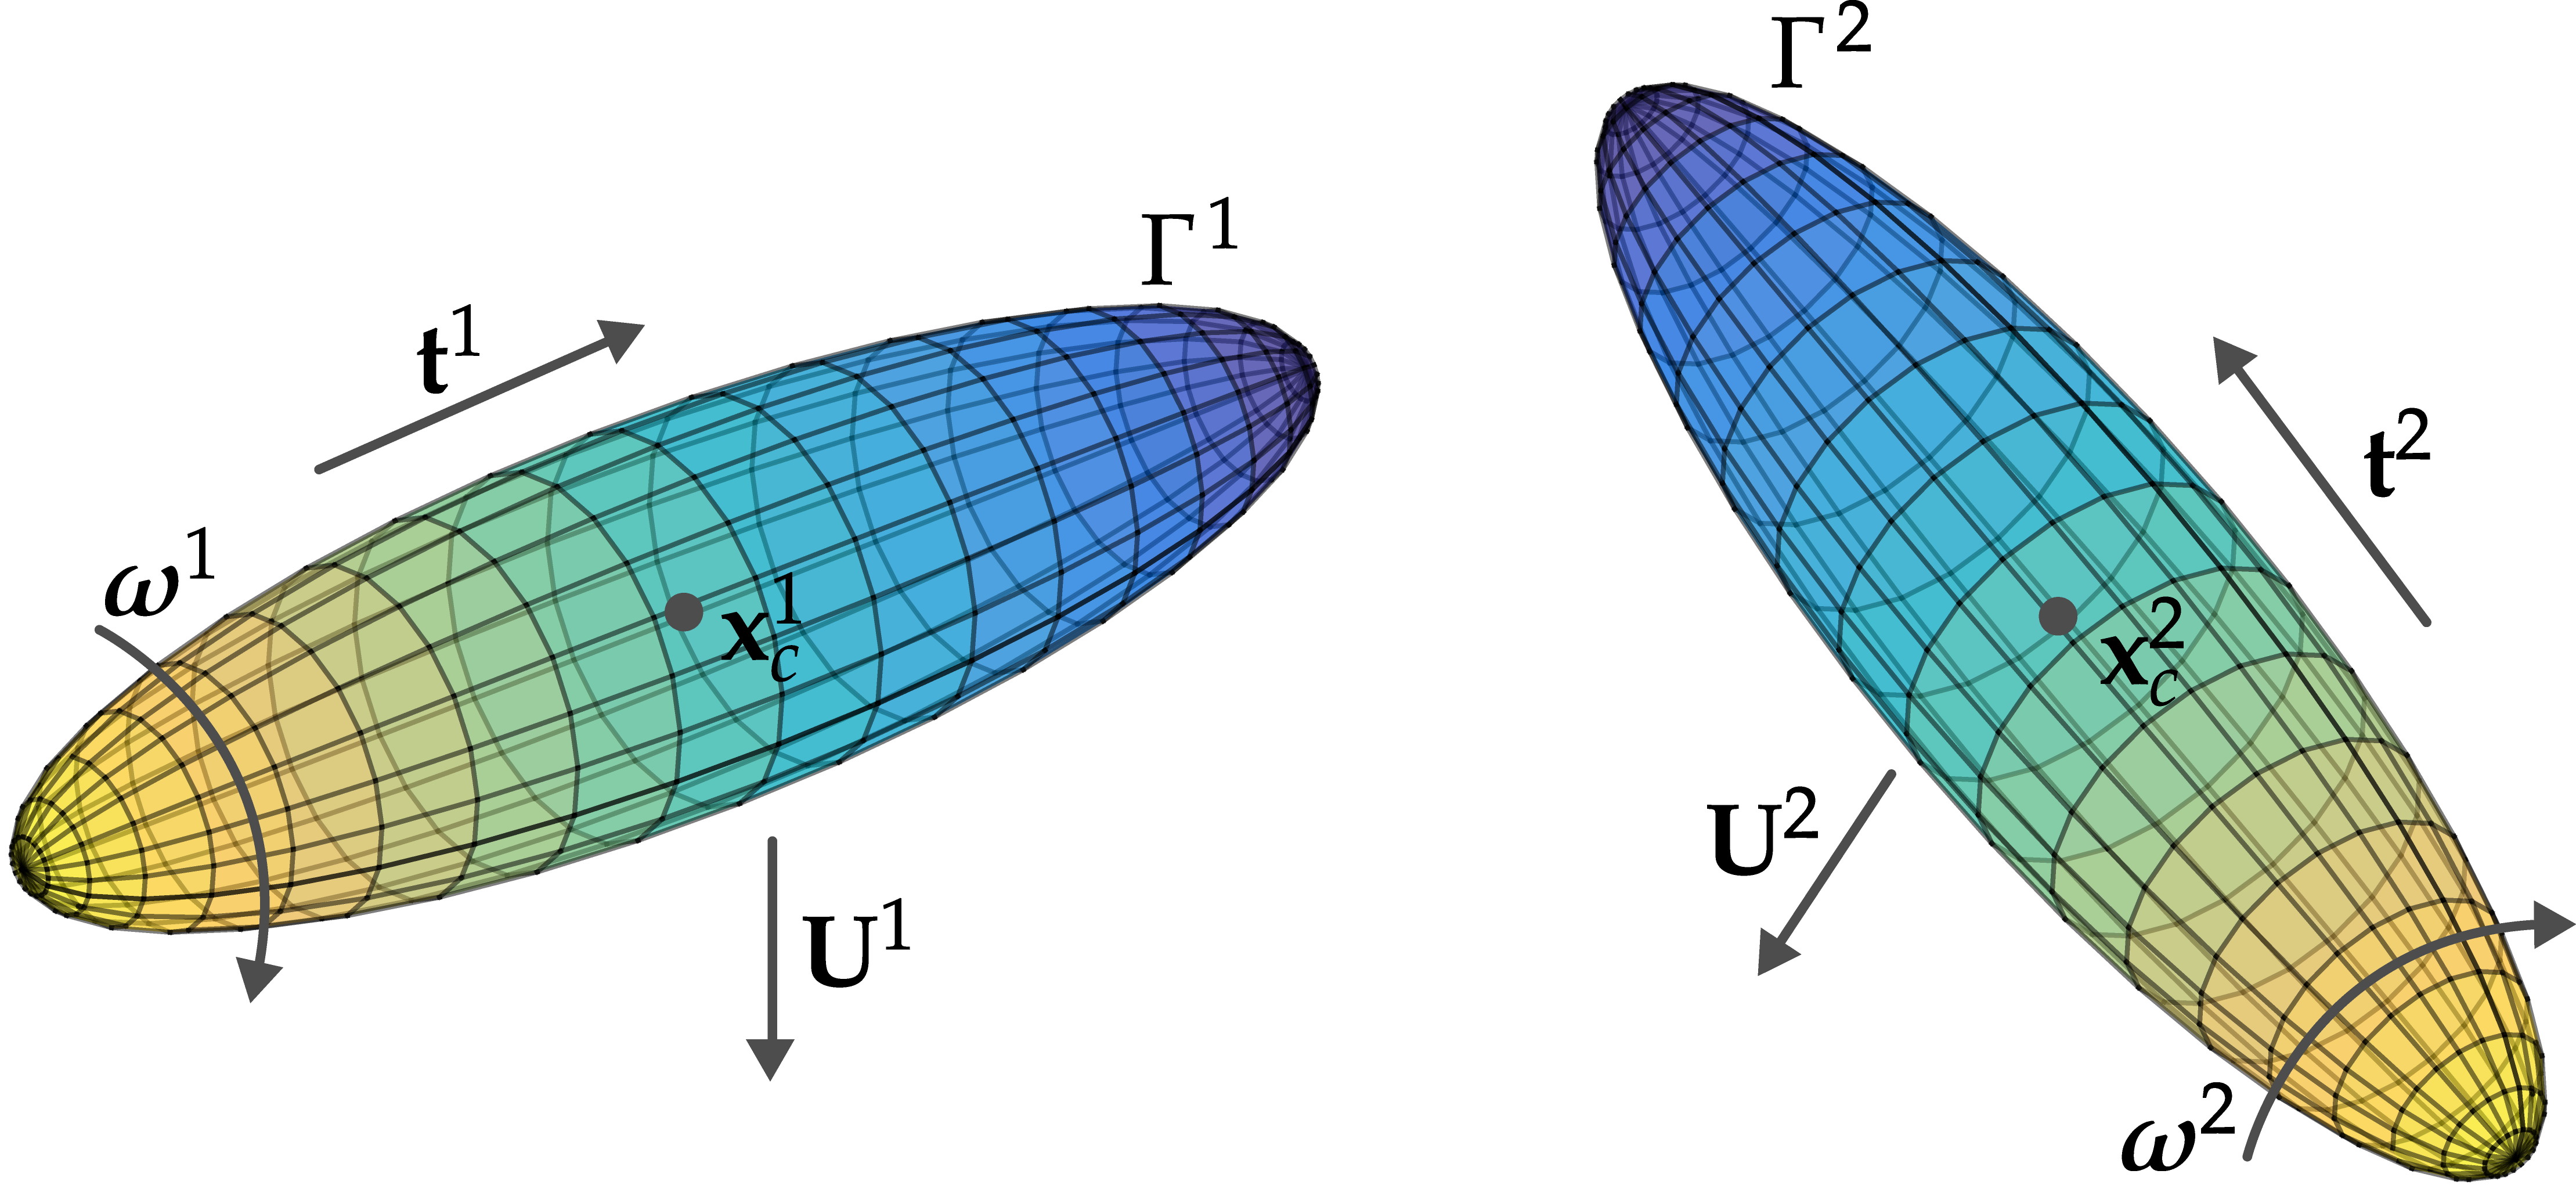
\includegraphics[width=.8\textwidth]{img/immersed_rigid.png}
  \caption[Two immersed objects in stokes flow.]{Two immersed objects in stokes flow, using a rigid body motion. Each fiber is characterized by the positions $\POS^1, \POS^2$ and the orientations $\ORIENT^1,\ORIENT^2$. The velocity of each point the surfaces $\Gamma^1, \Gamma^2$ is given by the rigid body motion described in Eqn~\eqref{eq:rigid_body_motion}.}
  \label{fig:immersed_rigid}
\end{figure}

By combining the rigid body motion with the boundary integral formulation (Eqn.~\eqref{eq:stokeslet_velocity_field}) of the Stokes equations we can now relate the objects velocities with the force exerted by all other objects. For this we take advantage of the linearity of the Stokes equation and apply the superposition principle. The superposition principle states that the combined effect from all objects at a single point in the flow is simply the sum of all the individual effects caused by each object. For $M$ fibers this yields the following relationship between the objects velocities and the force distribution , $f$, on the surface of the object,
\begin{equation}
  \label{eq:objects_boundary}
	\mathbf{U}_i^m + (\mathbf{\omega}^m \times (\POS - \POS_c^m))_i = \frac{1}{8 \pi \mu} \sum_{l=1}^{M} \int_{\Gamma^l} S_{ij}(\mathbf{x},\mathbf{y})f_j^l(\mathbf{y}) \, dS_y \quad i,j =1,2,3 \text{.}
\end{equation}

For a sedimenting object, the translational and rotational velocities $\mathbf{U}^m$ and $\mathbf{\omega}^m$ as well as the force distribution $\mathbf{f}^m$ are unknown. Thus in order to be able to solve the system we add two constraints
\begin{equation}
	\label{eq:objects_boundary_constraints}
	\mathbf{F}_{\text{object}}^m = \int_{\Gamma^m} \mathbf{f}^m(\mathbf{y}) \, dS_y\text{,} \quad \mathbf{T}_{\text{object}}^m = \int_{\Gamma^m} (\POS - \POS_c^m) \times \mathbf{f}^m(\mathbf{y}) \, dS_y \text{,}
\end{equation}
stating that the integrated force and torque over each object must be equal to the externally applied force and torque on the object. Given these additional constraints we are now able to solve Eqns.~\eqref{eq:objects_boundary} and~\eqref{eq:objects_boundary_constraints} for $\mathbf{f}^m$, $\mathbf{U}^m$ and $\mathbf{\omega}^m$ for all fibers $m=1,2,\dots,M$. Using the resulting velocities we can then update the position and orthonormal basis of each object through time $t$ by
\begin{equation}
	\label{eq:objects_update}
	\frac{d}{dt}\POS_c^m = \mathbf{U}^m \text{,} \quad \frac{d}{dt}\ORIENT^m = \ORIENT^m \times \mathbf{\omega}^m \text{.}
\end{equation}

Additionally, given the force distribution $\mathbf{f}_m$ of each fiber we can compute the velocity field $\mathbf{u}_i(\mathbf{x})$ at any point $\POS$ in the domain of interest of the Stokes flow. We again take advantage of the superposition principle and apply it to Eqn.~\eqref{eq:stokeslet_velocity_field} to express the velocity field as
\begin{equation}
	\label{eq:objects_velocity_field}
	\mathbf{u}_i(\mathbf{x}) = \frac{1}{8 \pi \mu} \sum_{l=1}^M \int_{\Gamma^l} S_{ij}(\mathbf{x},\mathbf{y})\mathbf{f}_j^l(\mathbf{y}) \, dS_y\text{.}
\end{equation}
The integral appearing in the right-hand side of Eqn.~\eqref{eq:objects_boundary} must in most cases be evaluated by numerical quadrature.

\section{Slender fibers}
\label{sec:slender_fibers}

The formulation developed in the previous section is now adapted for a particular rigid fiber suspension. Consider a straight, rigid body of length $2L$ and radius $a$, and let $\epsilon = a / 2 L$ denote a slenderness parameter. If $\epsilon \ll 1$ the body is referred to as a slender body (slender fiber) as illustrated in Fig.~\ref{fig:slenderness}.

\begin{figure}[!htbp]
  \centering
  \begin{subfigure}[h]{0.24\textwidth}
    \centering
    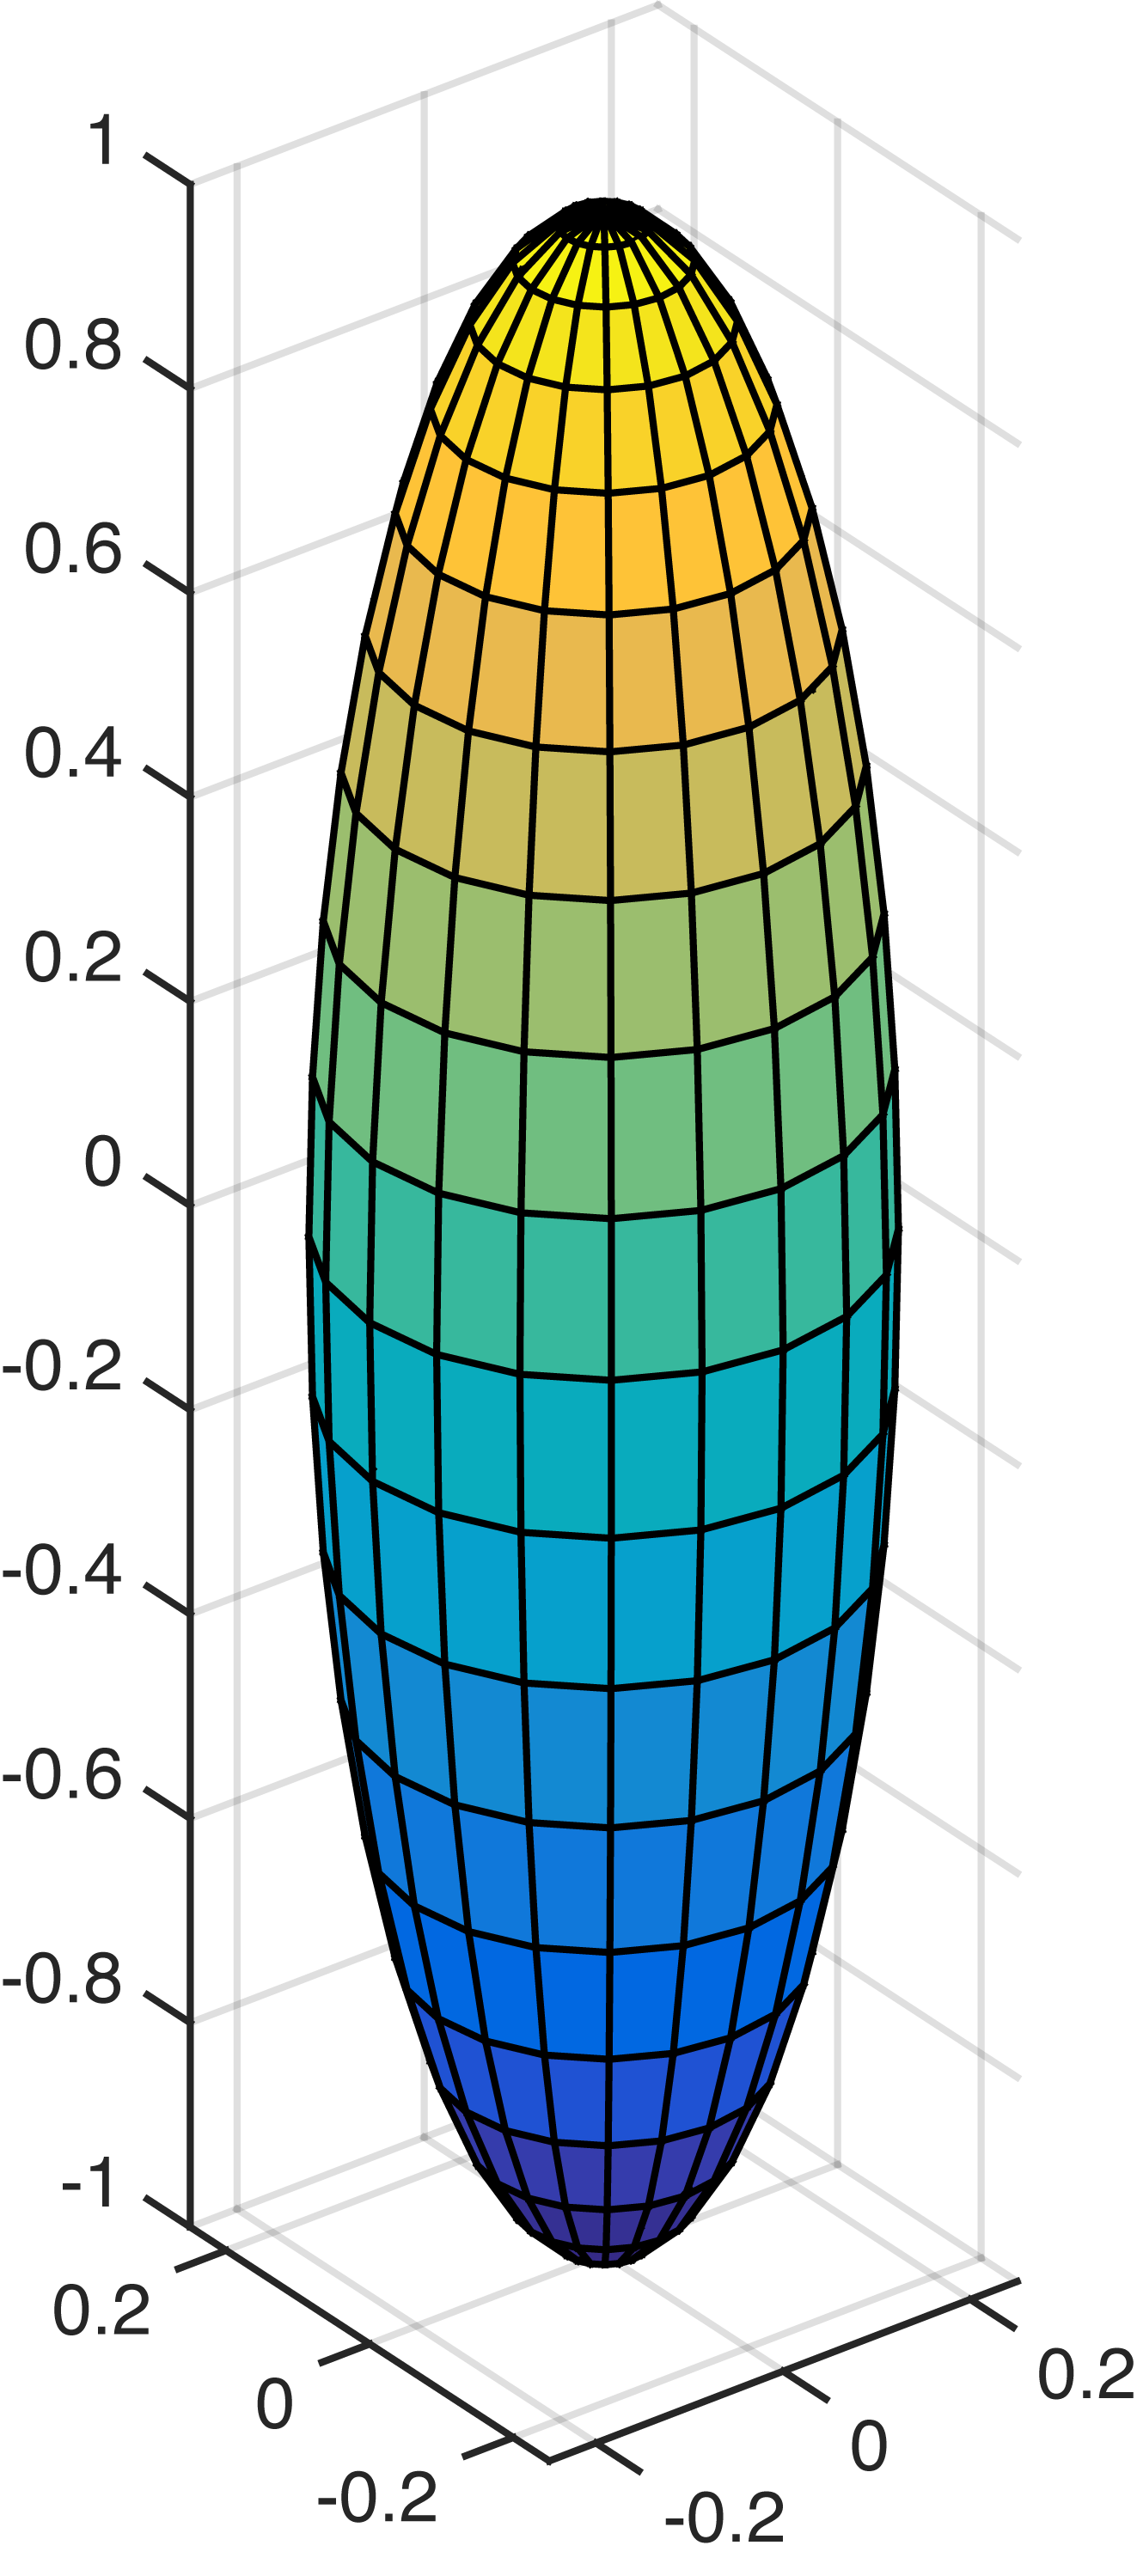
\includegraphics[width=\textwidth]{img/slender/1_4.png}
    \caption{$\epsilon=1/4$}\label{fig:slenderness_1_4}
  \end{subfigure}
  \begin{subfigure}[h]{0.24\textwidth}
    \centering
    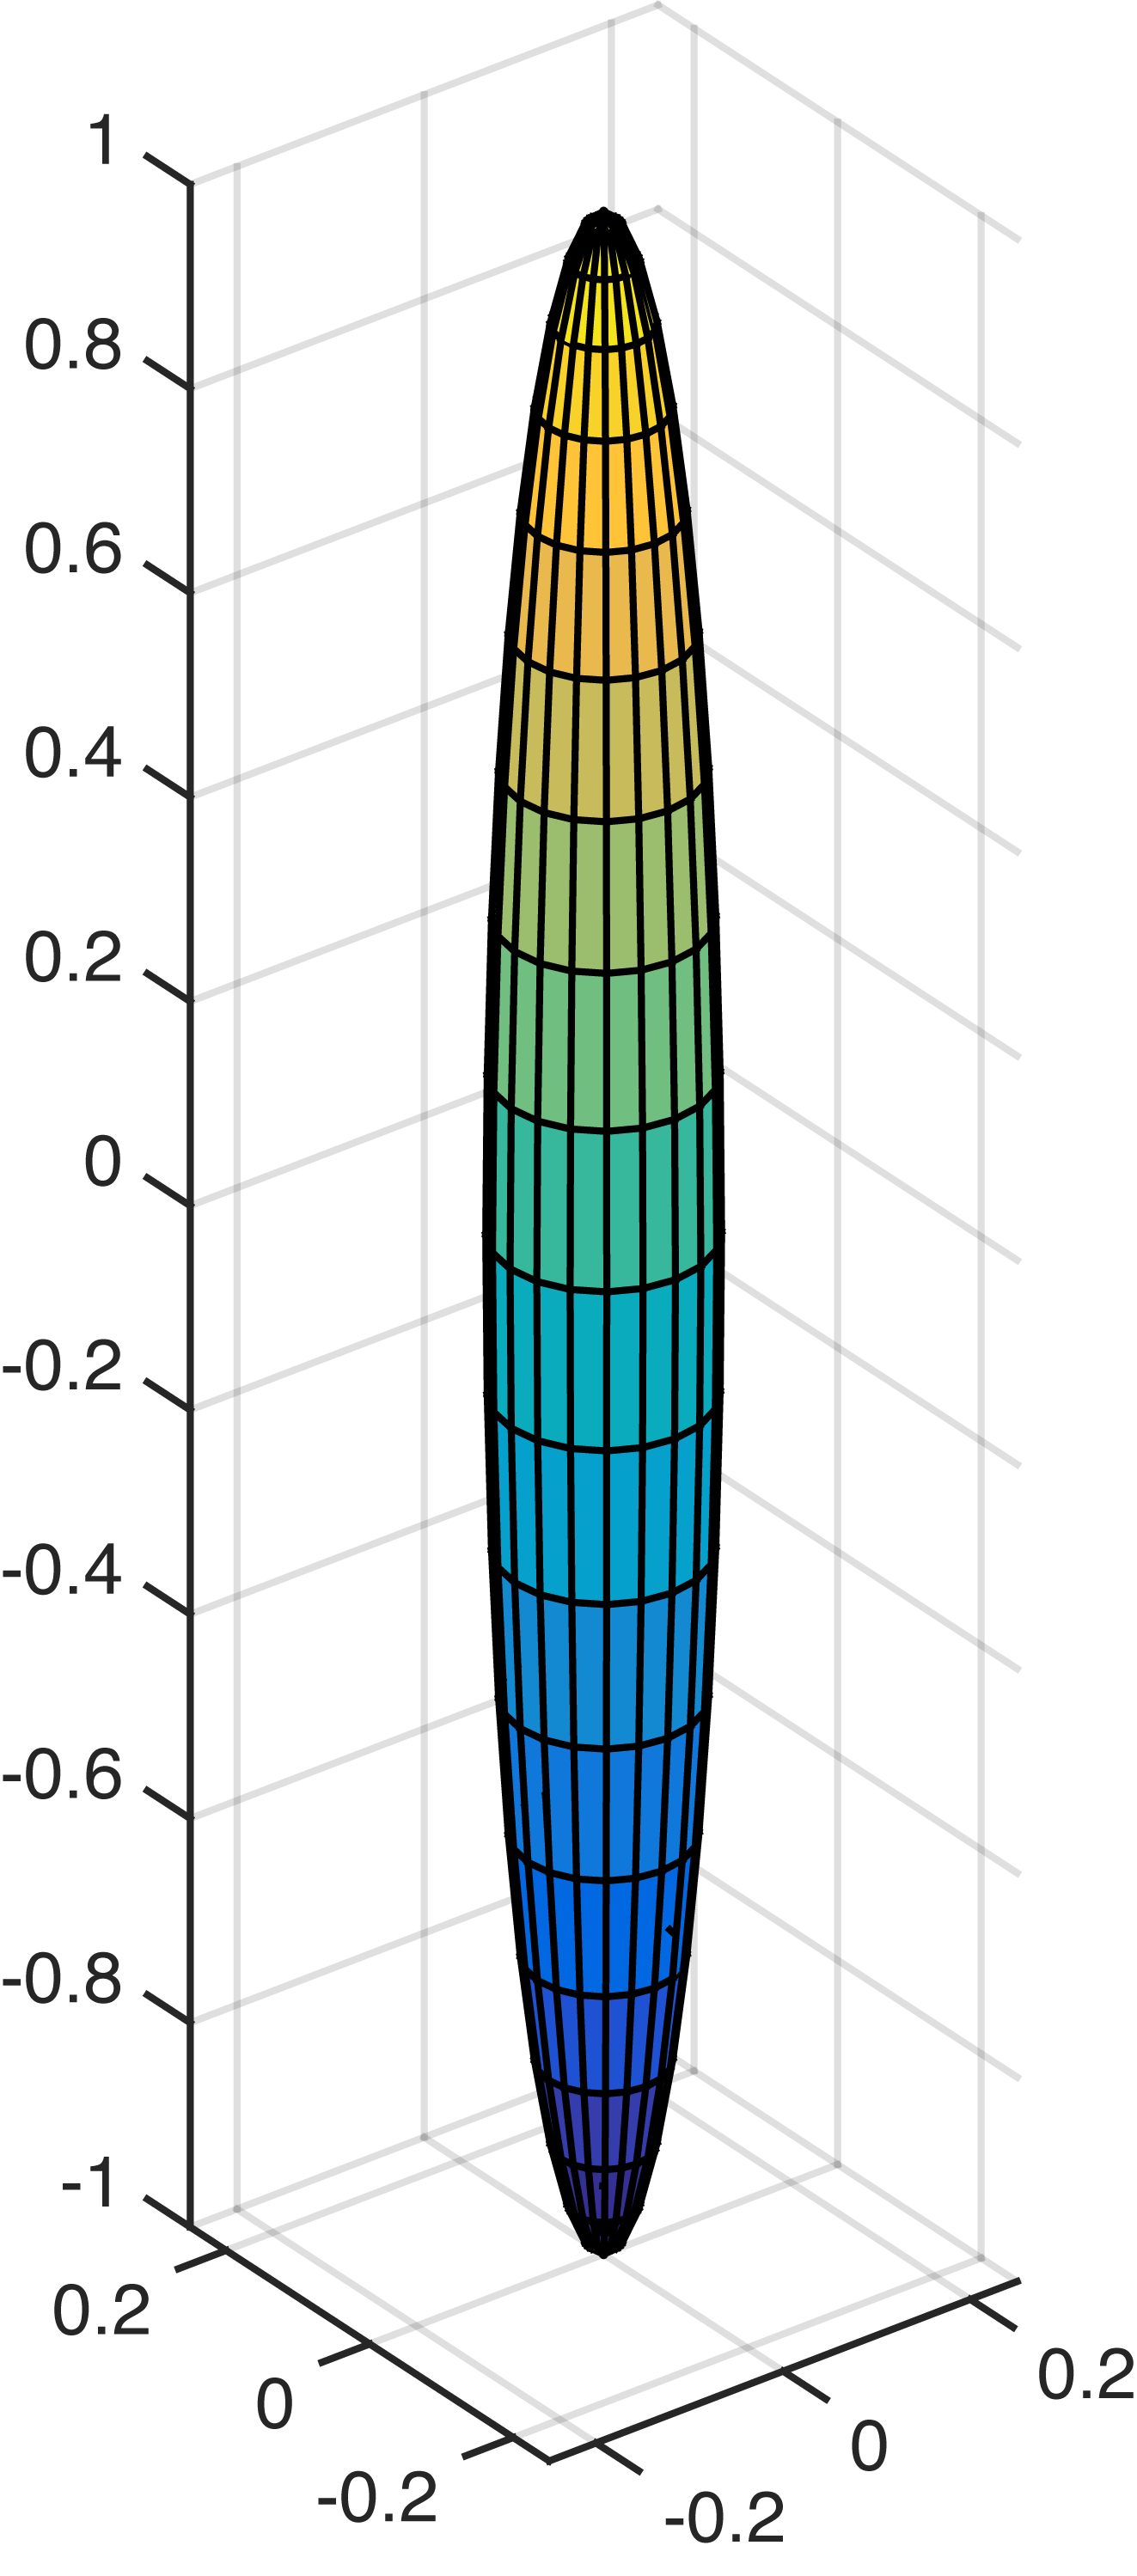
\includegraphics[width=\textwidth]{img/slender/1_10.png}
    \caption{$\epsilon=1/10$}\label{fig:slenderness_1_10}
  \end{subfigure}
  \begin{subfigure}[h]{0.24\textwidth}
    \centering
    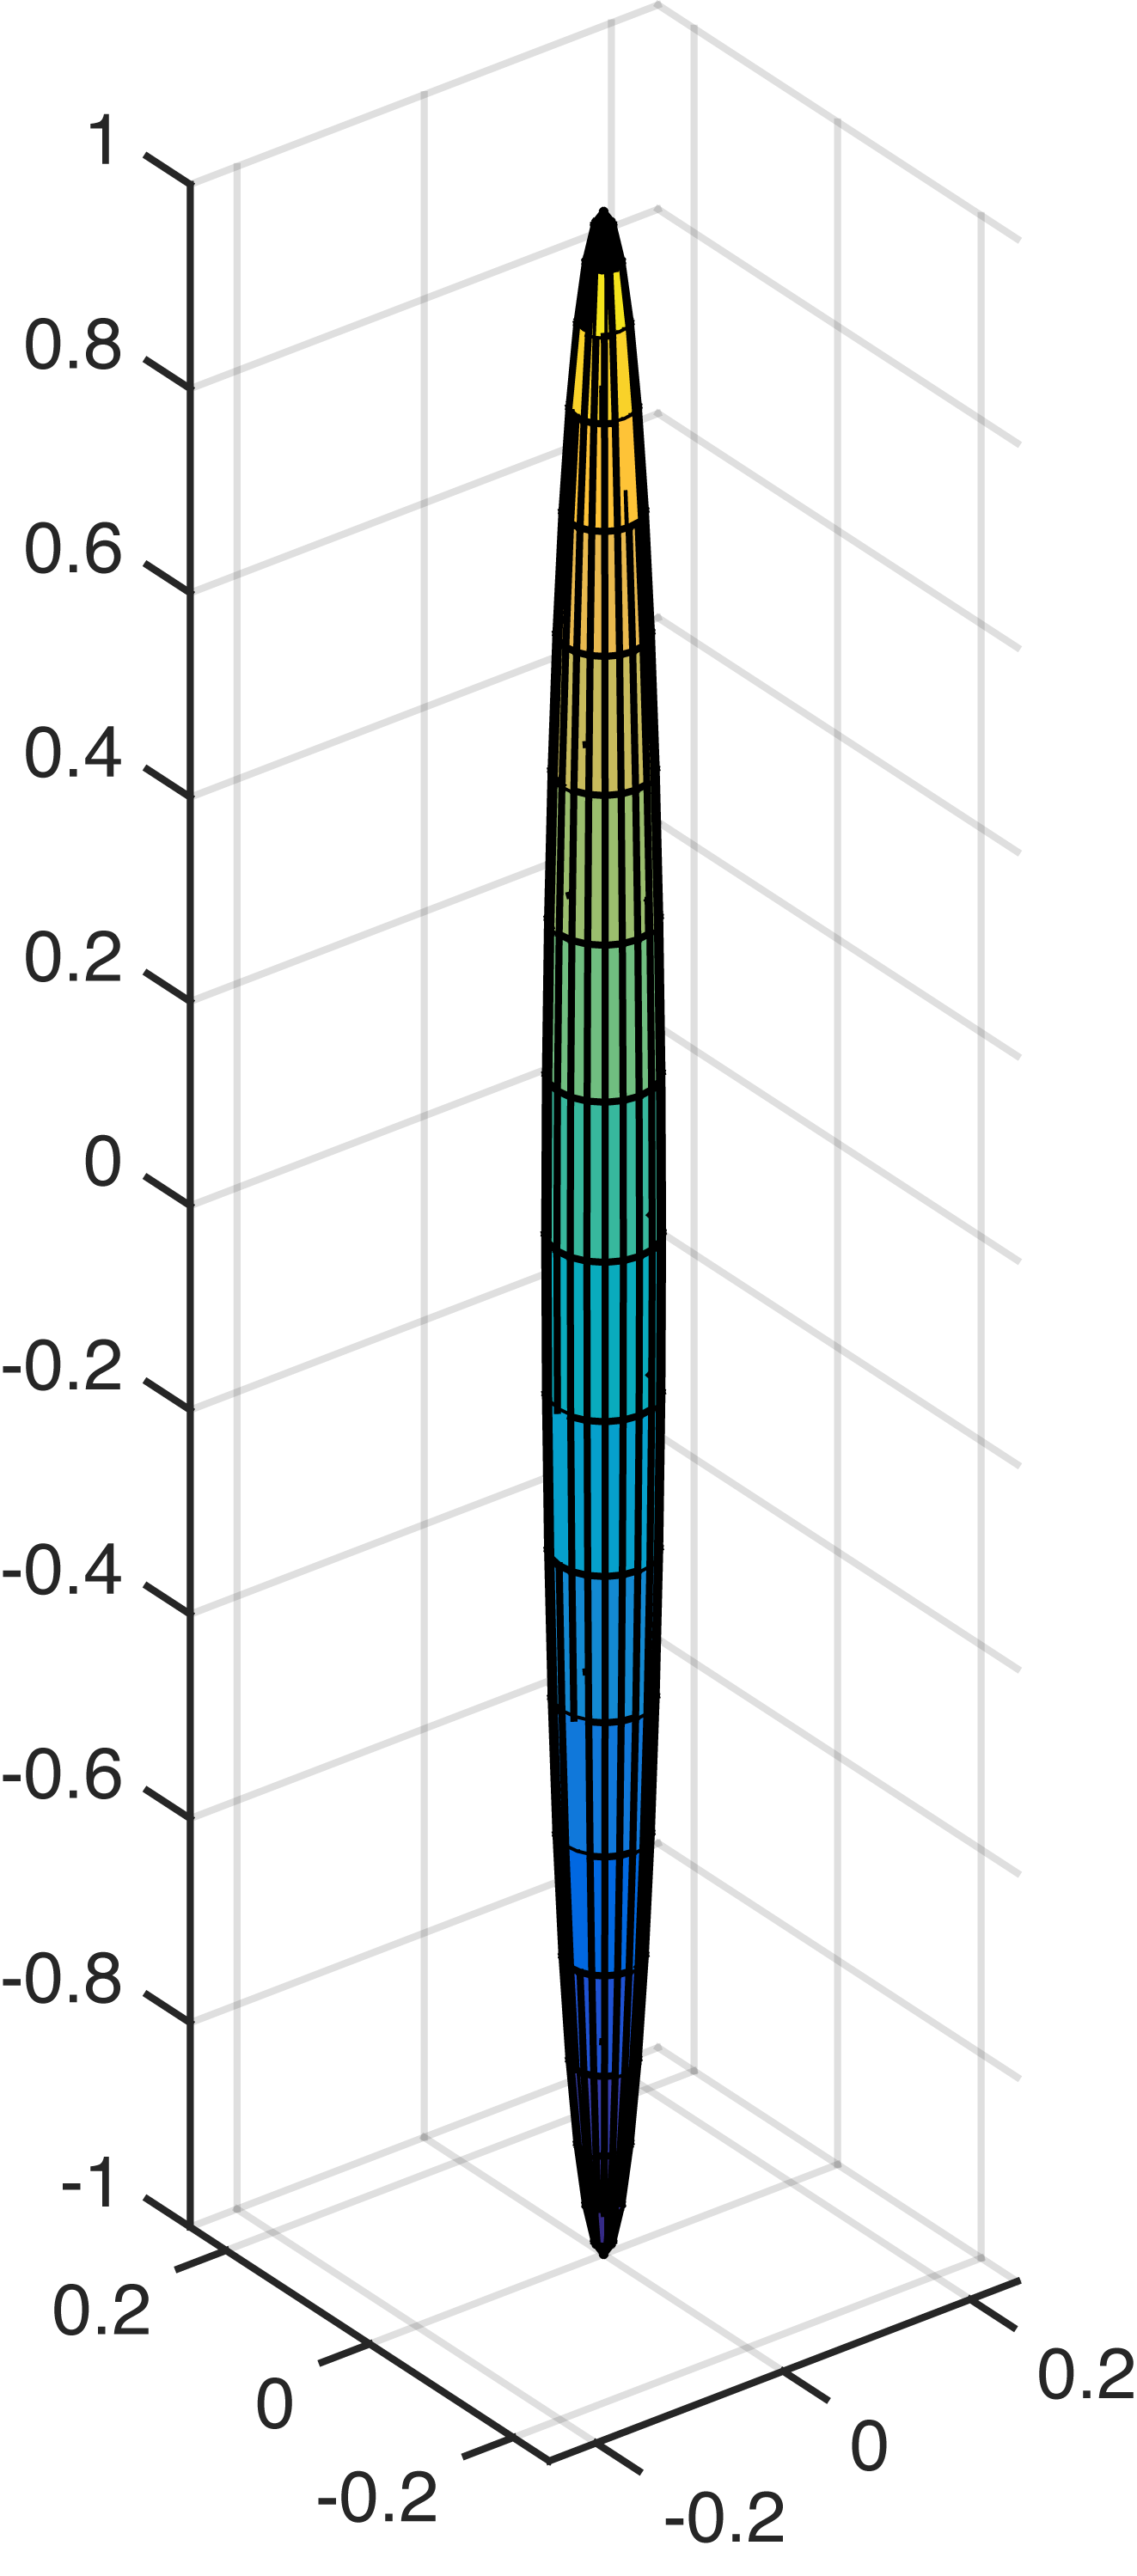
\includegraphics[width=\textwidth]{img/slender/1_20.png}
    \caption{$\epsilon=1/20$}\label{fig:slenderness_1_20}
  \end{subfigure}
  \begin{subfigure}[h]{0.24\textwidth}
    \centering
    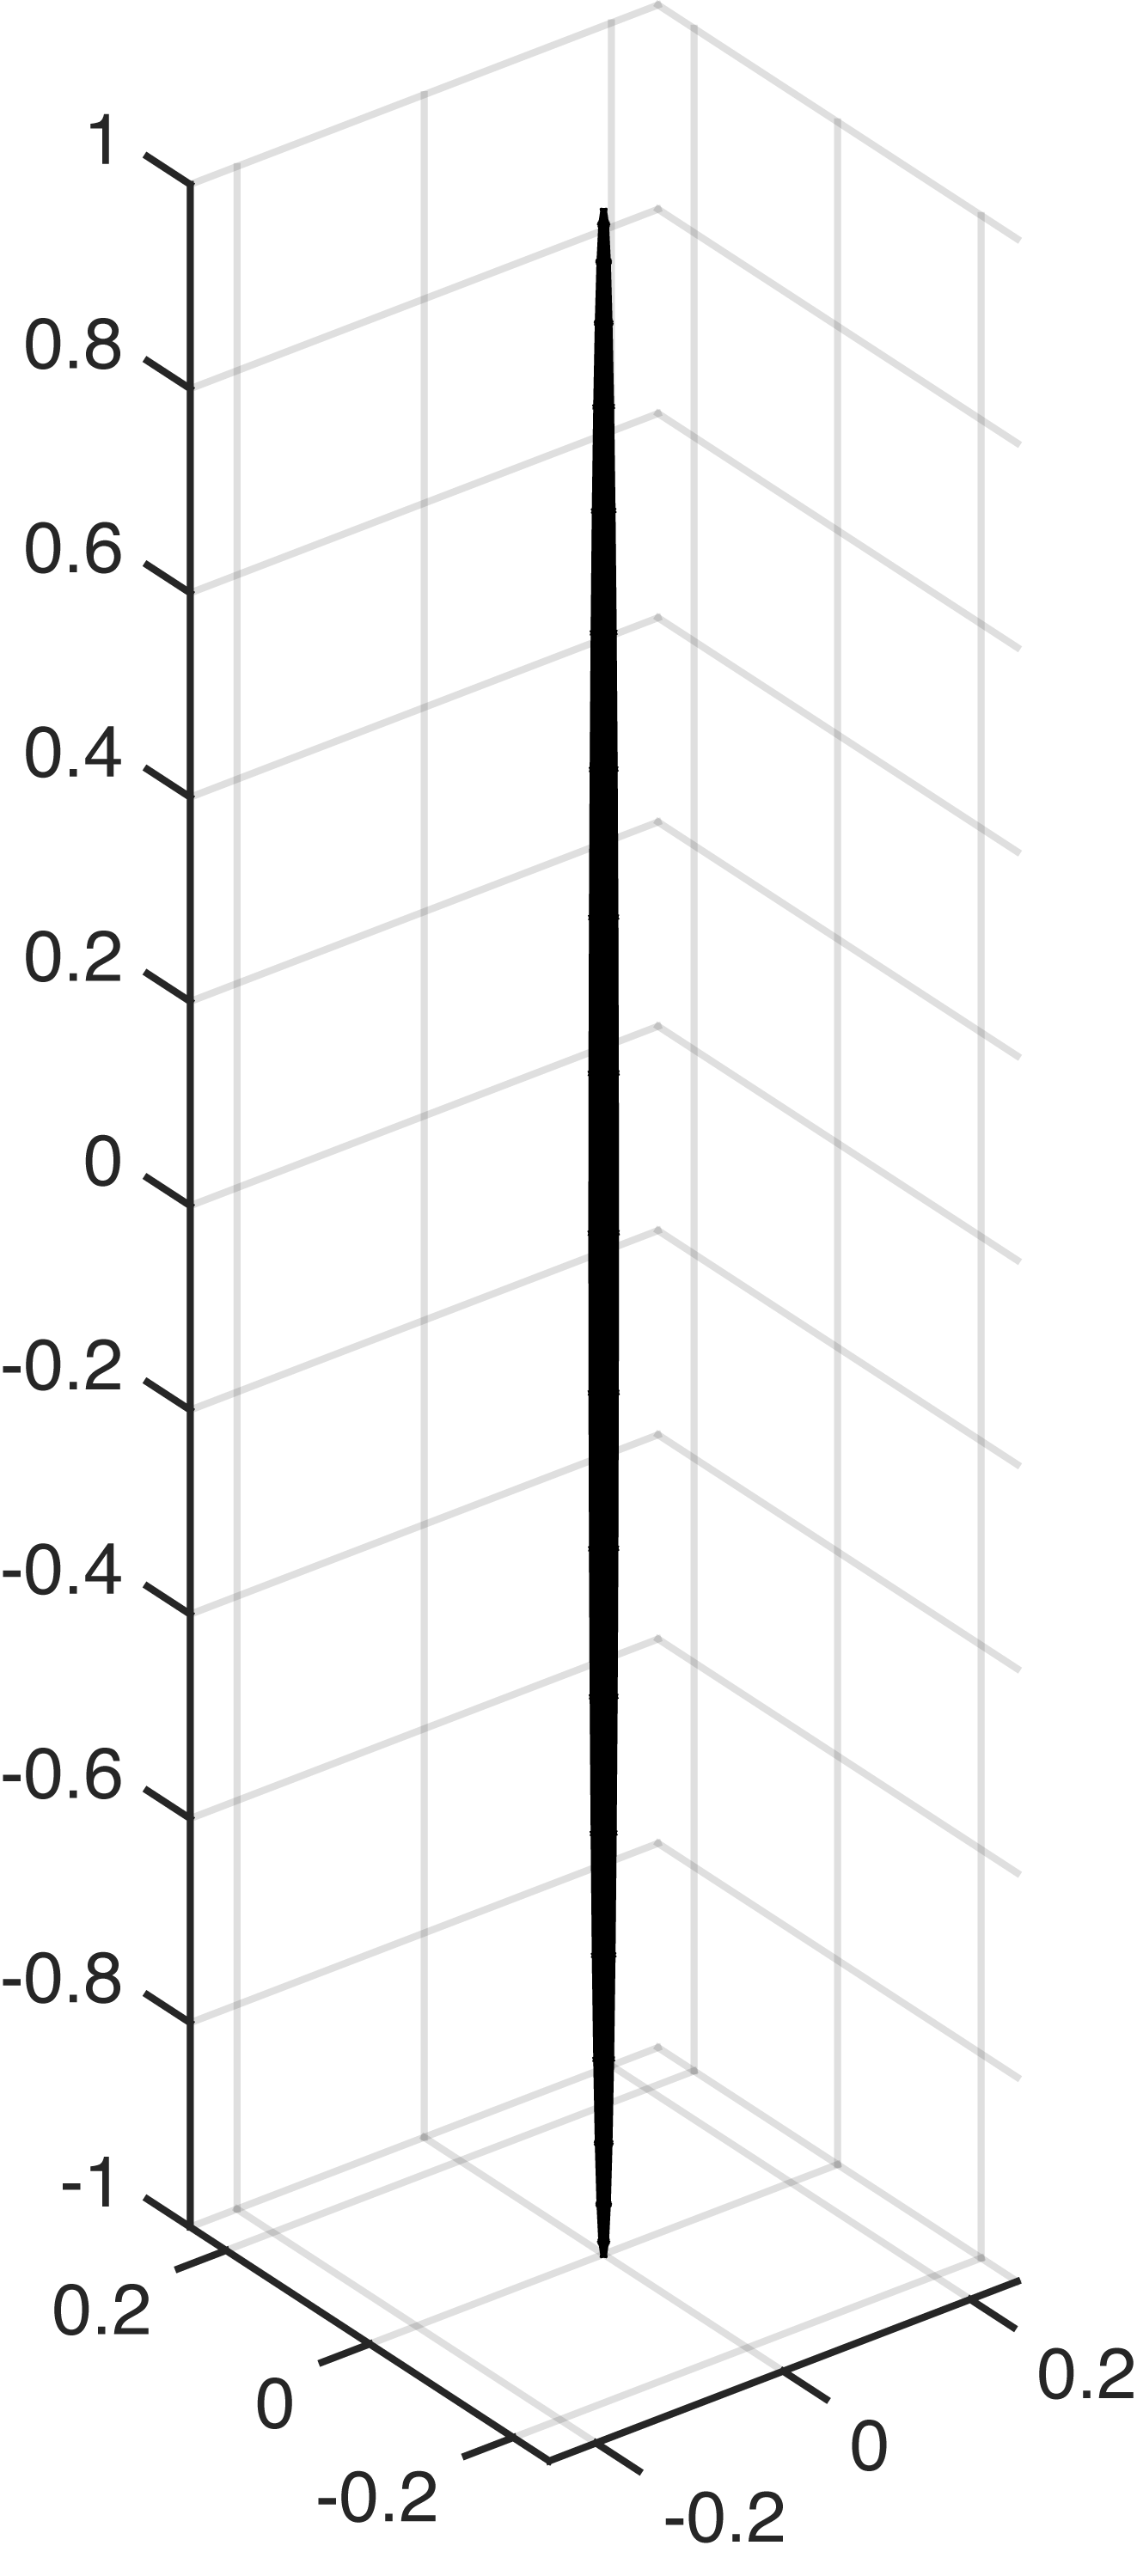
\includegraphics[width=\textwidth]{img/slender/1_100.png}
    \caption{$\epsilon=1/100$}\label{fig:slenderness_1_100}
  \end{subfigure}
  \caption[Illustration of the slenderness parameters.]{Illustration of the slenderness parameters, when $\epsilon$ becomes smaller the shape of the body asymptotically approaches that of an infinitesimal slender fiber.}
  \label{fig:slenderness}
\end{figure}

Our goal is to simulate many slender fibers, but using the 2D boundary integral formulation would be very expensive to solve numerically. As the aspect ratio $1/\epsilon$ of the fiber increases, the requirement of the number of quadrature points also increases in order to accurately resolve the flow field around the fibers. However, for slender bodies a slender body approximation can be used instead. 

The slender body approximation is derived from the boundary integral formulation of the Stokes Eqns.~\eqref{eq:objects_velocity_field}. Using asymptotic analysis the governing surface integrals are reduced to 1D equations along a centerline of the fiber. This is achieved by matching the fluid velocity at a virtual boundary of a slender ellipsoid to the fiber centerline velocity~\cite{Gotz2000}. The accuracy of this approximation is in $O(\epsilon).$ This reduction in dimensionality from 2D boundary integral equations to 1D integral equations is crucial for the ability to include a large number of fibers in the simulations.

The slender body approximation yields a coupled system of 1D integral equations over two fundamental solutions of the Stokes equations, the Stokeslet~(Eqn.~\eqref{eq:stokeslet_stokeslet}) and the Doublet~(Eqn.~\eqref{eq:doublet}). The coupled system relates the forces exerted on the fibers to their velocities and captures the non-local interaction of the fiber with itself (as mediated by the fluid), as well as with any other structures with the fluid, such as other fibers or external boundaries. The system of integral equations is solved using a boundary integral method. Details of the model are given by Tornberg and Gustavsson~\cite{Tornberg2006}.

\begin{figure}[!htbp]
  \centering
  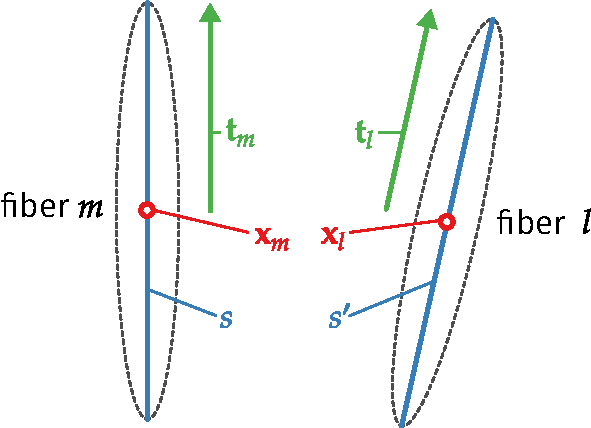
\includegraphics[width=0.5\textwidth]{img/slender.pdf}
  \caption[Slender fiber approximation.]{Slender fiber approximation. Each fiber is described by the center points $\POS_m, \POS_l$ the orientations given by the unit tangent vectors $\ORIENT_m, \ORIENT_l$ and the center line parameterized by $s$ and $s'$. The points of each center line is thus given by $\POS_m(s) = \POS_m + s\ORIENT_m$.}
  \label{fig:slender_fiber}
\end{figure}

Assume that we have $M$ fibers immersed in the fluid. As shown in Fig.~\ref{fig:slender_fiber} each fiber is now defined by its centerline and parameterized by the arc-length, $s \in [-L,L]$. For fiber $m$ the coordinates of the centerline are given by $\POS_m(s,t) = \POS_m(t) + s\ORIENT_m(t)$, where $\POS_m$ is the center point and $\ORIENT_m$ the unit tangent vector of the fiber and $m=1,2,\dots,M$.

If the fluid exerts a force per unit length, $\mathbf{f}_m$ on fiber $m$, the slender body approximation for the velocity of the centerline of fiber $m$ can be stated in non-dimensional form as
\begin{equation}
  \label{eq:velocity_centerline}
  \begin{aligned}
    d(\dot{\POS}_m + s \dot{\ORIENT}_m) &= \left[ d(\mathbf{I} + \ORIENT_m\ORIENT_m^\top) + 2(\mathbf{I} - \ORIENT_m\ORIENT_m^\top\right]\mathbf{f}_m(s) \\
    &+ (\mathbf{I} + \ORIENT_m\ORIENT_m^\top)\bar{\mathbf{K}}[\mathbf{f}_m](s) + \mathbf{V}_m(s) \text{.}
  \end{aligned}
\end{equation}
Here $d$ is a geometry parameter
\begin{equation}
  \label{eq:geometry_parameter}
  d = -\ln{\epsilon^2e} \text{,}
\end{equation}
and $\bar{\mathbf{K}}[\mathbf{f}_m](s)$ is an integral operator given by
\begin{equation}
  \label{eq:integral_operator}
  \bar{\mathbf{K}}[\mathbf{f}_m](s) = \int_{-1}^{1} \frac{\mathbf{f}(s') - \mathbf{f}(s)}{|s' - s|} \, ds' \text{.}
\end{equation}

The contribution to the velocity of fiber $m$ from the other fibers in the system is accounted for in $\mathbf{V}_m(s)$ as
\begin{equation}
  \label{eq:velocity_contribution}
  \mathbf{V}_m(s) = \sum_{l=1}^M \int_{-1}^{1} \mathbf{G}(\mathbf{R}_{lm}(s,s'))\mathbf{f}_l(s') \, ds' \text{,}
\end{equation}
where $\mathbf{R}_{lm}(s,s') = \POS_m + s\ORIENT_m - (\POS_l + s'\ORIENT_l)$ is the distance between one point on fiber $m$ and one point on fiber $l$ as illustrated in Fig.~\ref{fig:fiber_contribution}.

\begin{figure}[!htbp]
  \centering
  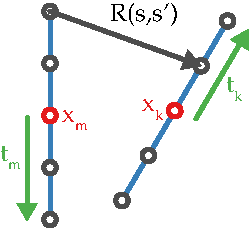
\includegraphics[width=0.3\textwidth]{img/fiber_contribution.pdf}
  \caption[Two interacting fibers with five quadrature points.]{Two fibers with five quadrature points each. The interaction between two fibers is given by the term $\mathbf{V}_m$ and depends solely on the distance between the two. The integral in Eqn.~\eqref{eq:velocity_contribution} can not be evaluated analytically and will be approximated by a quadrature rule.}
  \label{fig:fiber_contribution}
\end{figure}

The Green's function in this case is a linear combination of two fundamental solutions and reads
\begin{equation}
  \label{eq:green_function}
  \mathbf{G}(\mathbf{R}) = \begin{dcases*}
  \mathbf{S}(\mathbf{R}) + \frac{r^2}{2}\mathbf{D}(\mathbf{R}) & if $l \neq m$\\
  0 & if $l = m$
  \end{dcases*}
\end{equation}
with $\mathbf{S}$ and $\mathbf{D}$ as defined in Eqns.~\eqref{eq:stokeslet_stokeslet} and~\eqref{eq:doublet}.

In the non-dimensionalization the half-length of the fiber has been used as a characteristic length, $L_c = L$. This will give use a characteristic velocity and time as
\begin{equation}
  U_C = \frac{d \Delta \rho g V}{4\pi\mu_fL} \text{,} \quad T_C = \frac{2\pi\mu_fL^2}{d \Delta \rho g V} \text{.}
\end{equation}

The unknowns in Eqns.~\eqref{eq:velocity_centerline} are the translational and rotational velocities, $\dot{\POS}_m$ and $\dot{\ORIENT}_m$ and the force distribution along the fiber $\mathbf{f}_m(s)$. To close the formulation of Eqn.~\eqref{eq:velocity_centerline}, we use the additional conditions stating that the integrated force and torque on each fiber must balance the external forces and torques applied to the fibers,
\begin{equation}
	\label{eq:slender_boundary_constraints}
  \mathbf{F}_m = \int_{-1}^{1} \mathbf{f}_m(s) \, ds = \mathbf{F}_g \text{,} \quad \mathbf{T}_m = \int_{-1}^{1} s(\ORIENT_m \times \mathbf{f}_m(s)) \, ds = 0 \text{.}
\end{equation}

For our simulation the external force is just gravity and the external torque is set to zero. Together with this the system is now closed and we can solve our rigid fiber simulation using Eqns.~\eqref{eq:velocity_centerline} and~\eqref{eq:slender_boundary_constraints}.

\chapter{Numerical algorithm and serial implementation}
\label{cha:serial_implementation}

In the last chapter, we presented the theoretical foundation of the physics and mathematics involved in simulating rigid fibers. Based on the Stokes Equation, we introduced the framework of boundary integral methods to efficiently model the behavior of rigid fibers. Using this background we will now review the numerical approach used for the simulation.

We will separate the overall algorithm into four steps and discuss each step individually. Additionally, we will touch upon implementation details used in the original serial version. We close the chapter with a brief reflection of the performance characteristics of the serial implementation to guide the parallel implementation on the GPU.

\section{Discretization}
\label{sec:serial_discretization}
In the previous chapter we obtained the final closed system given by Eqns~\eqref{eq:velocity_centerline} and~\eqref{eq:slender_boundary_constraints}. In order to solve these equations we have to discretize them. For this we start by expanding the force as a sum of $N+1$ Legendre polynomials $P_n(s)$
\begin{equation}
  \label{eq:force_discretization}
  \mathbf{f}_m = \frac{1}{2}\mathbf{F}_g + \sum_{n=1}^{N}\mathbf{a}_{m}^{n} P_n(s) \text{,}
\end{equation}
where the coefficients $\mathbf{a}_m^n$ are vectors with three components. The number of Legendre polynomials $N$ used for the force expansion is a parameter and is set to $5$ in our simulation.

By algebraic manipulation of the integral equations~\eqref{eq:velocity_centerline} and~\eqref{eq:slender_boundary_constraints} and the use of the orthogonality properties of the Legendre polynomials, a linear system of equations for $\mathbf{a}_m^n$ for $m=1,2,\dots,M$ and $n=1,2,\dots,N$ which only includes computational quantities, can be obtained. Furthermore, two separate equations for the translational and rotational velocities of the fibers are obtained as 
\begin{align}
	\dot{\POS}_m &= \frac{1}{2d}\left[d(\mathbf{I}+\ORIENT_m\ORIENT_m) + 2(\mathbf{I}-\ORIENT_m\ORIENT_m)\right] \mathbf{F}_m + \frac{1}{2d} \int_{-1}^{1} \mathbf{V}_m(s) \, ds \text{,} \label{eq:delta_translate_velocity} \\
	\dot{\ORIENT}_m &= \frac{3}{2d}(\mathbf{I}-\ORIENT_m\ORIENT_m) \int_{-1}^{1}s\mathbf{V}_m(s) \, ds \text{.}\label{eq:delta_rotate_velocity}
\end{align}

Once the linear system of equations has be solved for $\mathbf{a}_m^n$, the forces on the fibers can be computed using Eqn.~\eqref{eq:force_discretization}. Using the forces, the position and orientation of the fiber can be updated by integrating equations~\eqref{eq:delta_translate_velocity} and~\eqref{eq:delta_rotate_velocity} in 
time. For more details and in-depth discussions please refer to the original paper by Tornberg and Gustavsson,~\cite{Tornberg2006}.

\section{Assemble System}

The first step of the algorithm is to compute and assemble the linear system of equations in memory. In the \emph{Assemble System} step all interactions between the fibers are computed. This is a very time consuming part of the algorithm since the computational cost is of $O(M^2)$.

Writing the system in a standard form $\mathbf{A}\mathbf{\bar{a}}=\mathbf{b}$ gives the following structure of the dense $3MN\times3MN$-matrix $\mathbf{A}$ and right-hand side $\mathbf{b}$,
\begin{equation}
  \label{eq:matrix_structure}
  \renewcommand\arraystretch{1.5}
  \mathbf{A} =
  \begin{bmatrix}
    \mathbf{I} & \bar{A}_{12} & \cdots & \bar{A}_{1M} \\
    \bar{A}_{21} & \mathbf{I} & \cdots & \bar{A}_{2M} \\
    \vdots & \vdots & \ddots & \vdots \\
    \bar{A}_{M1} & \bar{A}_{M2} & \cdots & \mathbf{I}
  \end{bmatrix} \text{,} \quad \mathbf{b} =
  \begin{bmatrix}
    \bar{b}_{1} \\
    \bar{b}_{2} \\
    \vdots \\
    \bar{b}_{M} \\
  \end{bmatrix} \text{.}
\end{equation}
In this notation $\bar{A}_{ml}$ describes the $3N\times3N$ matrix encapsulating the contribution from the force coefficients on fiber $l$ onto the force coefficients for fiber $m$.

\pagebreak
\paragraph{Inner integral}

For each $\bar{A}_{ml}$, a $3\times3$ matrix, $\Theta_{lm}^{kn}$, where
\begin{equation}
  \label{eq:inner_integral}
  \Theta_{lm}^{kn} = \int_{-1}^{1} \left[\int_{-1}^{1}\mathbf{G}(\mathbf{R}(s,s')) P_k(s') \, ds' \right]P_n(s) \, ds \text{,}
\end{equation}
has to be evaluated for each force index $k,n = 1,2,\dots,N$. $\mathbf{G}$ and $\mathbf{R}$ are defined as in Eqns.~\eqref{eq:green_function}~and~\eqref{eq:velocity_contribution}, respectively. One approach is to use a standard Gaussian quadrature for both the inner and outer integral. However, as fibers get very close to each other a large number of quadrature points are needed to accurately compute the fiber interactions. As the number of quadrature points increase the computational time increases as well. For our simulation we use the same approach as the original paper. We divide each fiber into 8 subintervals and use a three-point gaussian quadrature on each interval. This results in a total of $3 \times 8 = 24$ quadrature points per fiber, which represents a good trade-off between accuracy and performance.

Another option is to use an analytical solution for the inner integral and only solve the outer integral numerically. We will not discuss the detailed derivation of the analytical solution, for an in-depth discussion please see Tornberg and Gustavsson,~\cite{Tornberg2006}. In theory this approach allows for perfect accuracy for the inner integral, however in practice this is limited by the numerical precision of the simulation. The obtained formulas are recursive and sensitive to round off errors. To minimize the accumulation of round off errors, the original serial implementation uses a trick and switches the direction of the recursion, depending on how far apart the fibers are. This improves the practical accuracy and does not have a negative effect on the performance.

Choosing between both options requires a careful examination of the accuracy and performance trade-off and is dependent on the simulation setup. For the original serial implementation the combined numerical and analytical approach for evaluation proved to be the fastest and was thus chosen as the default. We will later explore how is applies to the new parallel GPU implementation.

\section{Solve system}

After having assembled the linear system $\mathbf{A}\mathbf{\bar{a}}=\mathbf{b}$ the next step to solve it. This can be done using standard linear equation solvers. This step is treated as a black box by the simulation, simply plugging in the matrix $\mathbf{A}$ and the vector $\mathbf{b}$ and getting back the solution vector $\mathbf{\bar{a}}$ representing the force coefficients.

The linear system can either be solved using a direct solver or an iterative method like GMRES. As long as the fibers are not too close to each other the matrix is well-conditioned and GMRES is able to solve the system in less than $10$ iterations. This is the reason why the original serial implementation uses GMRES by default. How the different solvers perform on the GPU will be compared in Sec.~\ref{sec:bench_linear_solvers}.

\section{Update velocities}

The force coefficients obtained by solving the linear system can now be used to calculate the right hand side in the separate equations for $\mathbf{\dot{x}}_m$ and $\mathbf{\dot{t}_m}$, Eqns.~\eqref{eq:delta_translate_velocity} and~\eqref{eq:delta_rotate_velocity}. The required implementation is similar to the computations for the \emph{Assemble System} step.

\section{Update fibers}
\label{sec:serial_update_fibers}

The final step takes care of advancing the fibers forward in time by solving Eqns.~\eqref{eq:delta_translate_velocity} and~\eqref{eq:delta_rotate_velocity}. These equations do not impose any strict stability restrictions, so an explicit time-stepping scheme can be used. We use the same second order multi-step method as used in the original paper. The update for the position of the center coordinate $\mathbf{x}_m$ is given by the following discretization in time
\begin{equation}
  \label{eq:time_discretization}
  \frac{3\mathbf{x}_m^{i+1} - 4\mathbf{x}_m^{i} + \mathbf{x}_m^{i-1}}{2 \Delta t} = (2\mathbf{\dot{x}}_m^{i} - \mathbf{\dot{x}}_m^{i-1}) \text{,}
\end{equation}
where the time step is denoted by $\Delta t$ and superscripts denote the numerical approximation of $\mathbf{x}_m(t_i)$. In order to compute the next state this method requires both the previous and the current state. As there is no previous time step for $t_0$, the first step $\mathbf{x}_{m}^{1}$ is computed by a simply first order forward Euler method. The calculation for the orientation vector $\mathbf{t}_m$ is computed using the same discretization by replacing the translational velocity $\mathbf{\dot{x}}_m$ with the rotational velocity $\mathbf{\dot{t}}_m$. Additionally, we must renormalize the orientation vector so that it maintains its unit length.

At the end of this step the state of the fibers can optionally be written to an external file for post processing and visualization in other tools. After completing this step, the algorithm starts again from the top with the \emph{Assemble System} step. This cycle repeats until a specified number of time steps have been executed.

\section{Algorithm summary}
\label{sec:algorithm_summary}

The original paper implemented this algorithm using Fortran. All computation were performed in double precision and executed using a single thread on the CPU. In summary the four steps of the algorithm are at each timestep $t=t^n$ given the fiber configuration in terms of position, $\POS_m$, and orientation, $\ORIENT_m$, 
\begin{description}
  \item[1. Assemble System] \hfill \\
Computes all interactions between fibers and yields the linear system ${\mathbf{A}\mathbf{\bar{a}}=\mathbf{b}}$
  \item[2. Solve System]  \hfill \\
Solves linear system, treated as black box
  \item[3. Update Velocities] \hfill \\
Computes velocities $\mathbf{\dot{x}}$ and $\mathbf{\dot{t}}$
  \item[4. Update Fibers] \hfill \\
Yields new fiber configuration at $t=t^{n+1}$
\end{description}

For the number of fibers used in this work ($500–2000$), empirical results show that the majority of the required computation time is spent on the 1.~\emph{Assemble System} and 3.~\emph{Update Velocities} steps. The time required for advancing the simulation state in step 4.~\emph{Update Fibers} is completely negligible. We will see later in Chapter~\ref{cha:benchmarks} that the same holds true for the new parallel implementation.

\section{Remarks concerning GPU implementation}

There are some remarks to be made before we turn our attention to the GPU implementation of the algorithm. The most important step to optimize is 1.~\emph{Assemble System}, since it is the most time consuming step. Fortunately it is well suited for parallelization. The fibers can be partitioned naturally across the compute units, where each unit is responsible for a subset of fibers. As the required computations for the 3.~\emph{Update Velocities}~step are similar to the computations made in the 1.~\emph{Assemble System}~step, it will also benefit from the optimizations. Additionally, we will look at how the two different options for solving the integral in Eqn.~\ref{eq:inner_integral}, either combined analytical and numerically or purely numerical, perform in the parallel environment.

Since we will not be writing our own implementation of linear solvers on the GPU we have only limited influence on the performance of the 2.~\emph{Solve System}~step. As we instead treat it as a black box we have to rely on the efficiency of pre-existing libraries. The only thing we can control is the choice of which library and solver to use. For direct solvers the computational time only depends on the number of unknowns and is approximately constant throughout a simulation. The performance of iterative solvers on the other hand is highly depend on the condition number of the matrix and thus unpredictable. In line with the original paper we will both test a direct solver and iterative solvers to get a better understanding of their respective performance behavior.



\chapter{GPU programming}
\label{cha:gpu_programming}

In the previous chapter the numerical algorithm and its serial implementation was presented. It discussed various implementation details which have to be considered to arrive at the most efficient implementation.

To further increase the efficiency modern GPUs offer a massively parallel architecture to accelerate many different applications. We will begin with a short introduction to general purpose computing on GPUs. Afterwards, different Application Programming Interfaces (API) for programming on GPUs are discussed regarding their advantages and disadvantages. The chosen API, CUDA, will be presented with its programming model at the end of this chapter.

\section{General purpose computing on GPUs}
In the beginning Graphics Processing Units were highly specialized pieces of hardware developed to exclusively improve the performance of real-time 3D graphics. However, in recent years GPUs have started to be used for running arbitrary code instead of being limited to graphics related computations. This allows for impressive performance increases across a wide range of different general purpose applications. A good overview of the evolution of GPU computing can be found in Owens et al.~\cite{Owens2008}.

The deciding factor for the performance is how well the application can be parallelized to take advantage of the massively parallel architecture of GPUs. This massive parallelism has lead to potentially large performance advantages of GPUs over CPUs as illustrated in Fig.~\ref{fig:gpu_performance}. It shows the year over year increase in the theoretical floating point operations per second (FLOP/s). The FLOP/s number is calculated by combining information of the number of compute units, frequency and memory bandwidth for both the CPU and GPU models. This does not necessarily translate to direct real world performance increases but tries to visualize the potential GPUs have.

\begin{figure}[!htbp]
  \centering
  \begin{tikzpicture}
    \begin{axis}[
      xlabel={Year},
      ylabel={GFLOP/s},
      date coordinates in=x,
      xticklabel={\year},
      date ZERO=2002-01-01,
      xtick={2002-01-01,2004-01-01,2006-01-01,2008-01-01,2010-01-01,2012-01-01,2014-01-01},
      xmin=2002-01-01,
      xmax=2014-01-01,
      ymin=0,ymax=5500,
      ]
      \addplot[color=set12_light,mark=*,mark options={fill=white}, very thick] table[x=Date,y=Double,col sep=comma,meta=Name] {charts/cpu_performance.csv};
      \addlegendentry{Intel CPU Double Precision}

      \addplot[
      scatter,
      visualization depends on=\thisrow{alignment} \as \alignment,
      nodes near coords,
      point meta=explicit symbolic,
      every node near coord/.style={anchor=\alignment},
      color=set13_light,
      mark=*,
      mark options={fill=white},
      very thick,
      every node near coord/.append style={font=\tiny},
      ] table[x=Date,y=Double,col sep=comma,meta=Name] {charts/double_gpu_performance.csv};
      \addlegendentry{NVIDIA GPU Double Precision}

      \addplot[
      scatter,
      visualization depends on=\thisrow{alignment} \as \alignment,
      nodes near coords,
      point meta=explicit symbolic,
      every node near coord/.style={anchor=\alignment},
      color=set12,
      mark=*,
      mark options={fill=white},
      very thick,
      every node near coord/.append style={font=\tiny},
      ] table[x=Date,y=Single,col sep=comma,meta=Name] {charts/cpu_performance.csv};
      \addlegendentry{Intel CPU Single Precision}
      \addplot[
      scatter,
      visualization depends on=\thisrow{alignment} \as \alignment,
      nodes near coords,
      point meta=explicit symbolic,
      every node near coord/.style={anchor=\alignment},
      color=set13,
      mark=*,
      mark options={fill=white},
      very thick,
      every node near coord/.append style={font=\tiny},
      ] table[x=Date,y=Single,col sep=comma,meta=Name] {charts/single_gpu_performance.csv};
      \addlegendentry{NVIDIA GPU Single Precision}

    \end{axis}
  \end{tikzpicture}
  \caption[Theoretical GFLOP/s]{Theoretical GFLOP/s. Year over year increase in theoretical floating-point operations per second for CPUs and GPUs~\cite{CudaProgrammingGuide}.}
  \label{fig:gpu_performance}
\end{figure}

The huge difference in performance between a GPU and a CPU mainly derives from the number of independent compute units. How a compute unit is exactly defined differs between architectures and vendors. On a CPU the number of compute units usually refers to the number of CPU cores. Each individual CPU cores is very fast, however, CPUs usually only have four, eight or maybe sixteen cores. In contrast to this, GPUs can have several hundreds of independent compute units. Each GPU compute unit can perform calculations in parallel and thus provides the opportunity to yield big performance improvements for high-throughput type computations. This is one reason why g general purpose computing on GPUs was introduced to the world of supercomputers. Over time, a growing number of supercomputers started supplementing their computing power with GPUs and some even rely exclusively on GPUs for their computations.

In order to take advantage of these new massively parallel architectures new API had to be developed. The two proposed APIs are OpenCL and CUDA. OpenCL is an open and cross platform standard maintained by the Khronos Group~\cite{OpenCL}. The same group is also responsible for its graphics focused counterpart OpenGL. OpenCL is not exclusive to GPUs, but instead tries to be a general abstract layer for different parallel architectures. This allows OpenCL code to be run not only on GPUs but also on CPUs. CUDA on the other hand is developed by NVIDIA exclusively for their line of GPUs.

\section{CUDA vs. OpenCL}

Choosing between OpenCL and CUDA is the first decision to be made when starting to implement a new project on GPUs. The main advantage of OpenCL is the ability to run on many different devices. All major players in the computing space provide an implementation on top of their platforms. Both Intel and AMD provide the API for their CPU and both AMD and NVIDIA have drivers available for their GPUs. However, this advantage can also be a disadvantage as the achievable performance might suffer from the abstraction across all platforms. The OpenCL framework is potentially not optimized for a particular device specific architecture. CUDA on the contrary is in theory highly optimized to achieve the best possible performance on NVIDIA's GPUs. In practice the difference can possibly be mitigated by spending the extra time to fine-tune the OpenCL implementation to the hardware's specific needs. Another disadvantage of OpenCL is the potentially outdated and inconsistent driver support for the various devices. This is especially true for NVIDIA who seem to have stopped updating OpenCL, still only supporting OpenCL 1.1 which was released back in 2010. Their main focus is on pushing CUDA and updating it to support all the feature in their new GPUs.

For this thesis we chose to go with NVIDIA's CUDA framework mainly because of the available hardware both at the workstation computers and at the local computing cluster. Additionally, this project does not need the cross-platform capability as the main focus is on pure performance in a highly specialized setup and simulation scenario. The application will not be widely distributed and only used for internal purposes.

\section{CUDA programming model}
\label{sec:CUDA}
The abbreviation CUDA stands for Compute Unified Device Architecture and was introduced by NVIDIA in 2006 as a general purpose parallel computing platform. It leverages the highly parallel architecture of modern NVIDIA GPUs to solve many different computational problems, which can lead to potentially large performance improvements compared to traditional CPUs.

The CUDA platform allows developers to use a variety of different options to program the GPU. The easiest way is to link to any CUDA-accelerated library and simply using the libraries interfaces from any software environment. For more advanced uses extensions to various programming languages exist like C/C++, Fortran and even managed languages like Java, Python and many more. This allows for easy and fast integration into any software environment the developer is comfortable with. Fig.~\ref{fig:cuda_overview} illustrated the different components of the overall CUDA platform.

\begin{figure}[!htbp]
  \centering
  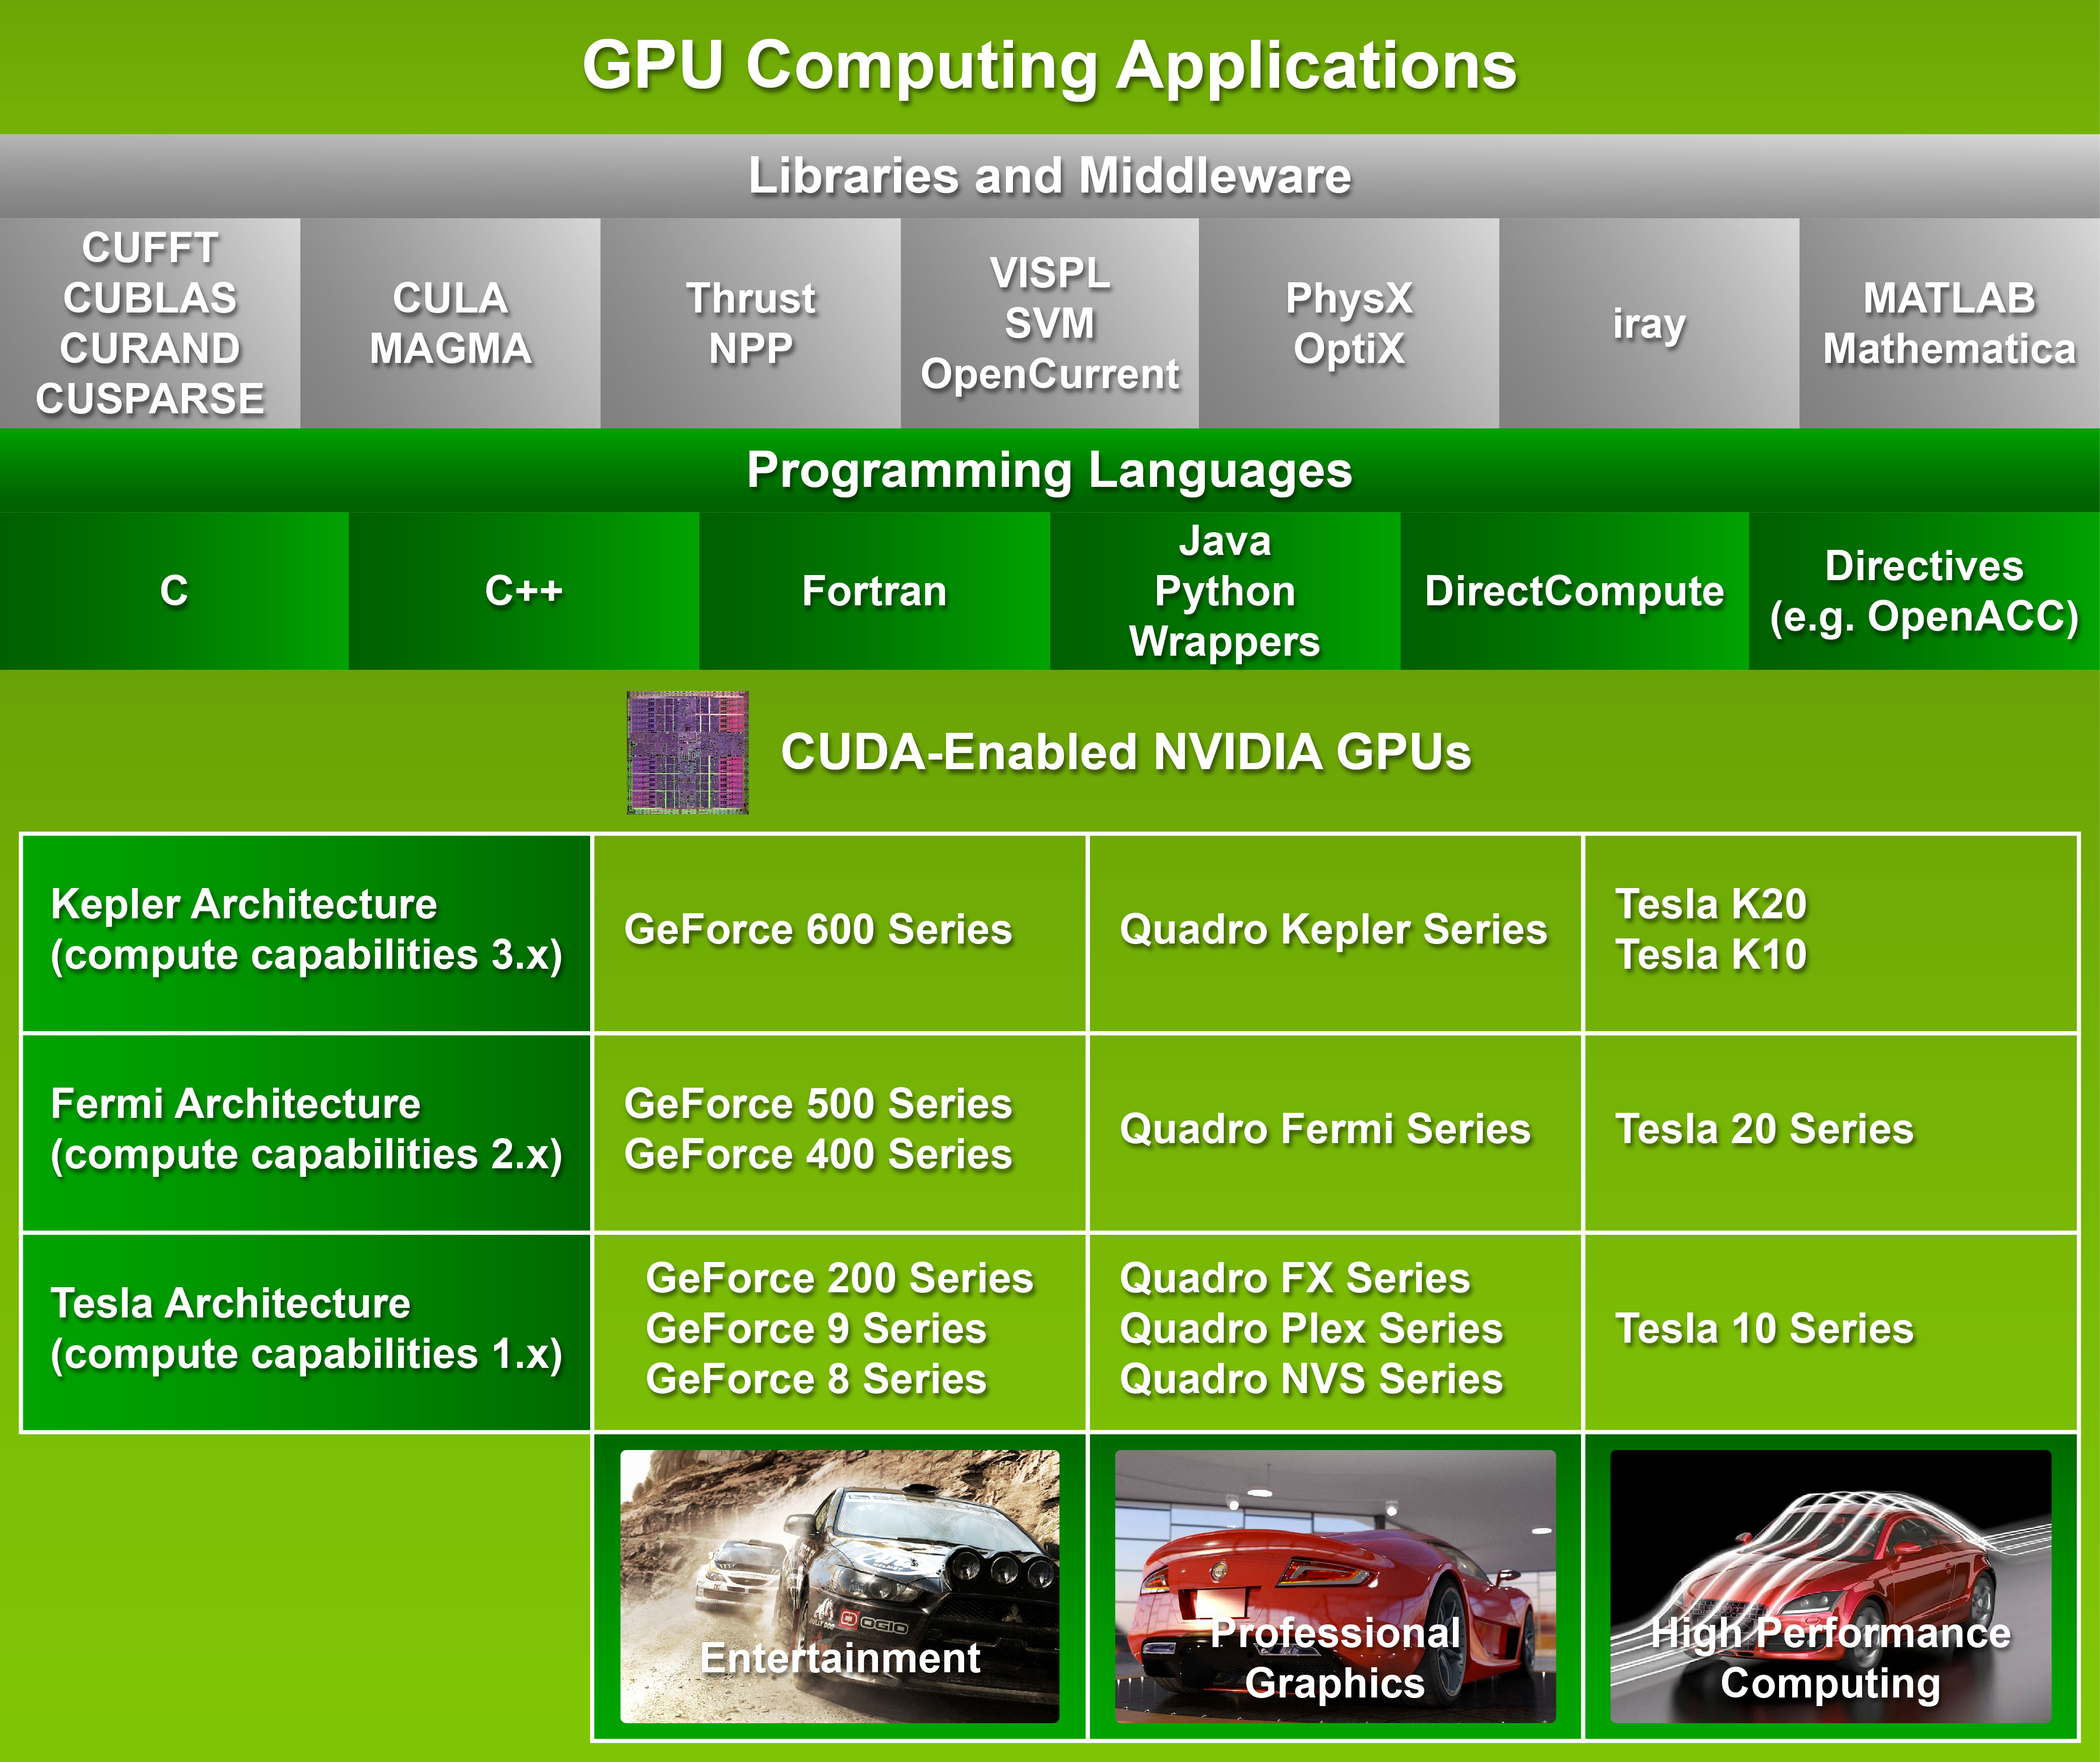
\includegraphics[width=.9\textwidth]{img/cuda_overview.jpg}
  \caption[Overview of the CUDA platform.]{Overview of the CUDA platform~\cite{CudaProgrammingGuide} describing the available libraries, programming environments and application of general purpose computing using CUDA.}
  \label{fig:cuda_overview}
\end{figure}

The basic building blocks of the CUDA Programming Model from a development perspective are kernels. CUDA kernels are the equivalent of normal C functions. However, the major difference is that instead of being executed just once, kernels are executed in parallel by $N$ different threads. These CUDA threads are distributed and run across the available compute units of the GPU. To illustrate how a very basic kernel invocation looks, Listing~\ref{lst:code_vector_addition} shows a code sample for a very simple vector addition.

\begin{listing}[!htbp]
  \centering
  \inputminted[mathescape,
    linenos,
    numbersep=5pt,
    fontsize=\footnotesize,
    frame=lines,
    framesep=2mm]{c}{lst/cuda_vector_add.lst}
  \caption{Pseudocode for CUDA vector addition.}
  \label{lst:code_vector_addition}
\end{listing}

\paragraph{CUDA kernels}

It is important to remember that each kernel invocation is executed independently and no ordering is guaranteed. It is therefore essential to avoid any order-dependent operations or shared memory access. There are however, ways to allow for shared memory access which will be briefly touched upon later in the practical implementation of the simulation.

\paragraph{Thread hierarchy}

In order to efficiently distribute the different threads across the compute units of the GPU, CUDA defines a thread hierarchy. As discussed previously a GPU consists of many independent compute units. On NVIDIA GPUs these units are referred to as Streaming Multiprocessors (SMs). During execution of the application each SM is tasked with running a distinct set of threads. In CUDA these sets of threads are called thread blocks. Each thread block is distributed to all the available SMs, which allows for automatic scalability depending on the number of SMs available  as illustrated in Fig.~\ref{fig:automatic_scaling}. Thus the developer only has to divide the workload into appropriately sized blocks of threads and invoke the kernel.

\begin{figure}[!htbp]
  \centering
  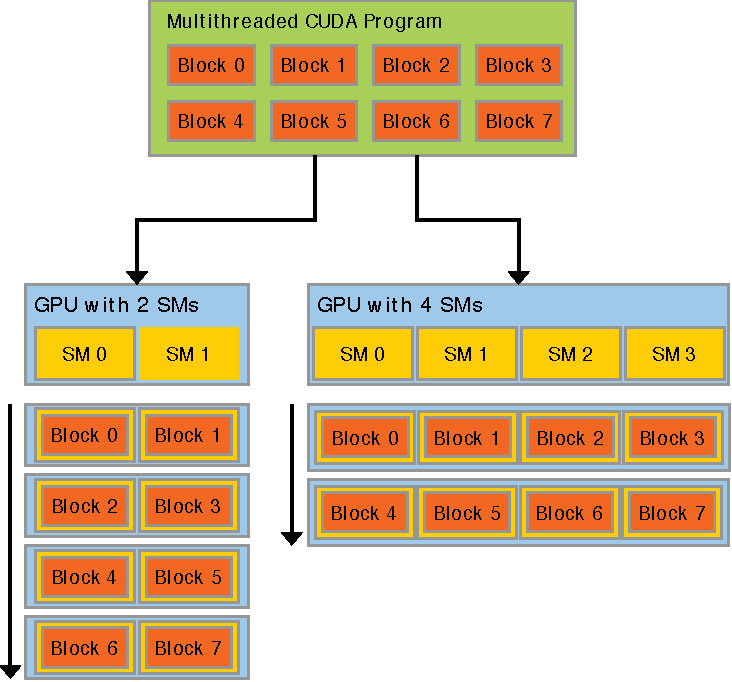
\includegraphics[width=\textwidth]{img/automatic_scaling.pdf}
  \caption[Automatic scaling of blocks across an arbitrary number of Streaming Multiprocessors.]{Automatic scaling of thread blocks across an arbitrary number of Streaming Multiprocessors~\cite{CudaProgrammingGuide}.}
  \label{fig:automatic_scaling}
\end{figure}

How to choose the optimal size of a block in order to maximize the performance is not an easy question to answer and it is highly dependent on the particular task and implementation. In practice the size is often chosen by running benchmarks with various sizes to determine the optimal configuration.

In order to make programming easier, CUDA blocks can be addressed using either a one-dimensional, two-dimensional, or three-dimensional thread index. For example in the case of a calculation involving matrices, it is more natural to think about parallelizing each element given by the row and column index instead of a single one-dimensional index. This is illustrated in the code sample in Listing~\ref{lst:code_matrix_addition}

\begin{listing}[!htbp]
  \centering
  \inputminted[mathescape,
    linenos,
    numbersep=5pt,
    fontsize=\footnotesize,
    frame=lines,
    framesep=2mm]{c}{lst/cuda_matrix_add.lst}
  \caption{Pseudocode for CUDA matrix addition, illustrating 2D thread blocks.}
  \label{lst:code_matrix_addition}
\end{listing}

Finally, as the resources of each Streaming Multiprocessor are limited, there is an upper bound of how many threads a block can contain. Currently this maximum number of threads is $1024$. This means that the maximum size of matrices, that can be added with the two-dimensional thread block code sample in Listing~\ref{lst:code_matrix_addition} is $32\times32 = 1024$. To solve this problem CUDA introduces another layer above blocks called a grid. A grid organizes thread blocks again into either one, two, or three dimensions. The number of thread blocks in a grid is unlimited and thus solely dependent on the size of the workload. Fig.~\ref{fig:grid_blocks} shows an example configuration of a 2D grid with 2D blocks.

\begin{figure}[!htbp]
  \centering
  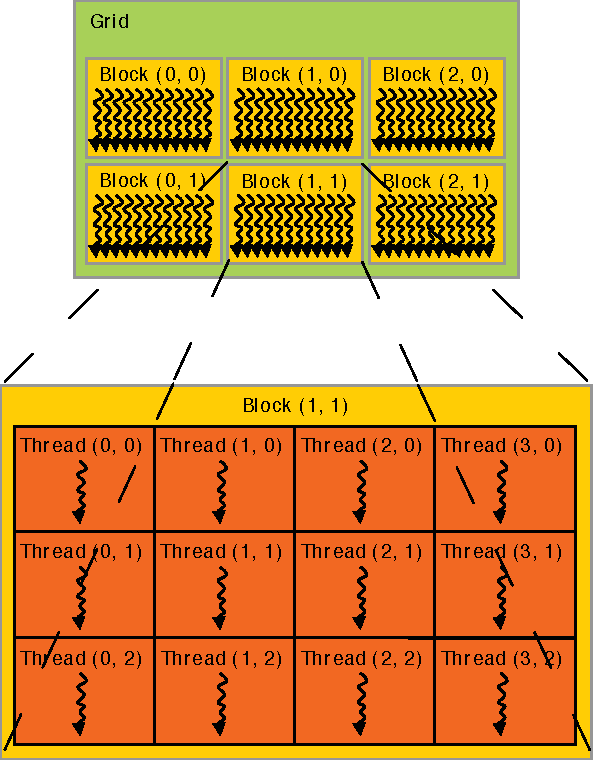
\includegraphics[width=0.6\textwidth]{img/grid_blocks.pdf}
  \caption[CUDA block addressing using 2D grid with 2D thread blocks.]{CUDA block addressing using 2D grid with 2D thread blocks~\cite{CudaProgrammingGuide}.}
  \label{fig:grid_blocks}
\end{figure}

\paragraph{Memory hierarchy}

In addition to the \emph{Thread Hierarchy} CUDA also implements a 3 layer memory hierarchy as illustrated in Fig.~\ref{fig:memory_hierarchy}. Each level of this hierarchy differs in size, latency and scope. The sizes refers to amount of bytes that can be stored in the level and latency to the time it between requesting data and being able to actually use it. Additionally each level is confined to a specific scope, restricting from where the data can be accessed.

The first level contains the fastest and smallest memory. This is a private memory where each thread has its own area and only this thread can read from and write to this area. How much space each thread has is determined by how many threads are executed on each SM. The more memory an individual thread requires the fewer threads can run in parallel on a SM. Optimizing this trade-off is important for achieving a good performance. On the newest GPUs each SM has $65536 * 32\text{-bit} = 256\text{KB}$ to divide among the threads.

The second level is called shared memory, or sometimes local memory. Although it is slower than the private memory, it has the advantage that all threads executing on an SM have simultaneous access to it. This allows different threads to cooperate and share work. Depending on the characteristics of the algorithm, this can save a lot of computing time. Therefore it is important to analyze whether shared memory can actually improve the performance. The size of this memory level on current GPUs is around $64\text{KB}$ to $96\text{KB}$.

The third level contains the largest memory area which is called the global memory. This is the amount of memory used  on the packaging of the GPUs to advertise the product. Nowadays it is usually $2\text{GB}$ or $4\text{GB}$. It is accessible by all threads and stores all data relating to the current application. However, accessing it can be quite slow compared to the other levels of the memory hierarchy. Additionally, one has to be careful to avoid memory conflicts when accessing the same memory location form different threads at the same time. This is especially important since this can further reduce the performance. Taking everything into account, it can be said that it is an important optimization step to make access to global memory as efficient as possible. This can be achieved by intelligently packing data, or caching data in a lower level of the hierarchy. 

Another option to avoid the slow the performance of the global memory is to make sure that the required data for each individual thread from global memory is small enough. The associated latency when reading data from global memory can be hidden when enough calculation are performed on this data. The GPU is then able to quickly switch to another set of threads and continue the computation while waiting on data from global memory.

\begin{figure}[!htbp]
  \centering
  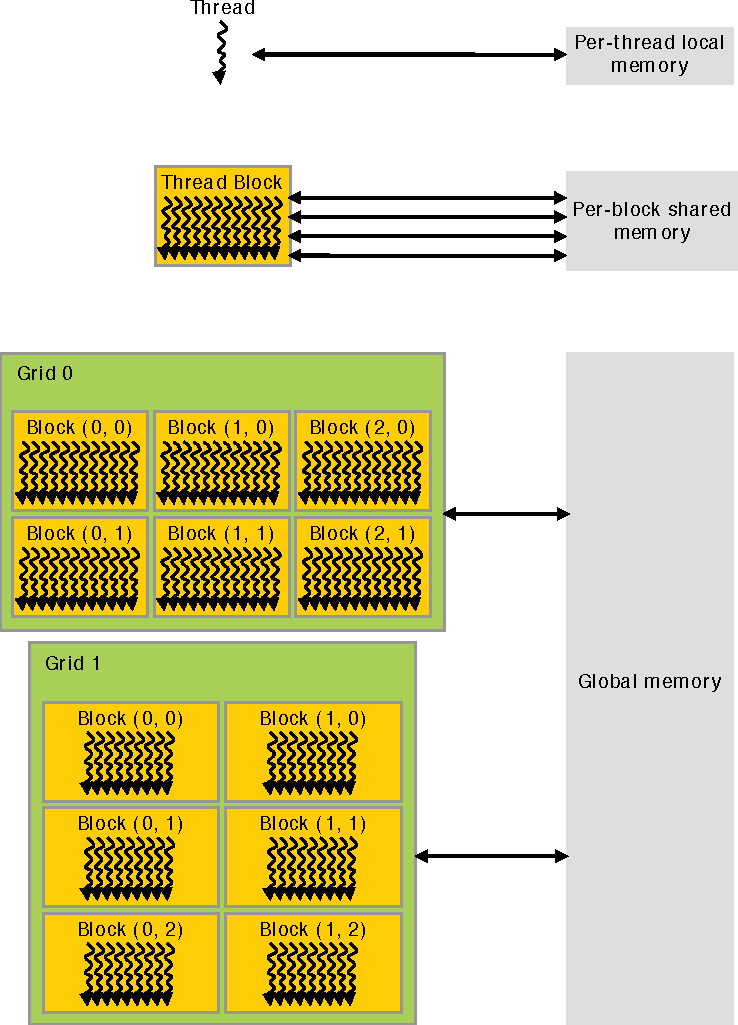
\includegraphics[width=0.8\textwidth]{img/memory_hierarchy.pdf}
  \caption[CUDA memory hierarchy.]{CUDA memory hierarchy~\cite{CudaProgrammingGuide}. The hiearchy consists of three layers (private, shared, global). Each layer differs in size, latency and scope.}
  \label{fig:memory_hierarchy}
\end{figure}


\chapter{Parallel Implementation}
\label{cha:parallel_implementation}

Based on the previous two chapters describing the serial Fortran implementation and GPU programming we will now look at the algorithm in more detail and show, how it was adapted to take advantage of multi-core architectures. The main focus of this thesis is the implementation of the simulation on a modern massively parallel NVIDIA GPUs using CUDA. In order to gain a better understanding of the achievable performance improvements we additionally back-ported the finished GPU code of the algorithm to multi-core CPUs using the OpenMP framework.

We will begin by introducing the software tools and libraries utilized. Afterwards, we will explain the practical implementation of the algorithm in CUDA. This is followed by the discussion of several potential optimization approaches to further improve the performance of the simulation. The chapter ends with a brief explanation of OpenMP and how the code was parallelized on the CPU.

\section{Development environment}

The rigid fiber simulation developed as part of this thesis is only loosely based on the original serial Fortran implementation. This was done to ensure a clean starting point and avoid difficulties in adapting the existing code for parallel execution, as it was never intended to be run across multiple cores. This also provided the opportunity to learn from the shortcomings of the old code to not only parallelize it but also improve the efficiency in general.

The development was done exclusively on a Linux workstation running Ubuntu as this will also be the exact same runtime environment used in the later experimental usage of the resulting application. The build system for compiling and linking the final application was CMake. It was chosen because it is a widely used open-source and cross-platform build system, which allows for easy integration of the various required libraries in a well documented and straightforward manner.

Under the hood the build system uses NVIDIA's CUDA platform tools to compile the code. For this NVIDIA includes \emph{nvcc}, an LLVM-based CUDA compiler capable of compiling C/C++ code together with the CUDA specific extensions.

In order to facilitate easier usage of the application both during development and later real-world usage a Python wrapper script is also available. The script completely automates the building process and dynamically customizes the application code to support three different modes of operation. The first is a simple \emph{run} mode which takes the supplied parameters and executes the simulation. The second mode is \emph{validate}, it allows for a fully automated way to test and validate different algorithm variations against a known correct simulation run. This includes automatically computing the error as well as the error location in the matrix allowing for easier debugging of changes. The last mode is \emph{benchmark} which runs the supplied parameters through a series of iterations collecting and aggregating timings for each simulation step as well as the total time.

\section{Linear Solvers}
In addition to the CUDA platform, the application also requires support libraries for the different linear solvers. It is very important to weigh all the options when choosing a particular linear solver algorithm or library, because solving the system can be one of the most time consuming steps. So the overall simulation time relies heavily on the ability to solve large and dense systems as fast as possible. The two main libraries are \emph{MAGMA} for the direct solver and \emph{ViennaCL} for the iterative solvers. Both will be introduced briefly now.

\paragraph{MAGMA / CuBLAS / OpenBLAS}
The MAGMA project contributes the implementation for the direct solver used in this thesis. This dense linear algebra library provides features similar to standard LAPACK functions but for multicore architectures. It also has features to support hybrid algorithms to run code across multiple GPUs or CPUs at the same time, however, these features were not explored in this thesis. Instead the focus was on a high performance single GPU implementation of a direct linear system solver.

MAGMA provides access to various high-level algebra routines, but the underlying math functions utilize the platform specific implementations of the BLAS levels. For CUDA this is implemented directly by NVIDIA in the form of the CuBLAS libraries. Additionally, MAGMA tries to further improve their performance by combining GPU with CPU based algorithms. Thus a CPU based BLAS implementation is also needed. For this the OpenBLAS library was chosen which is the most up-to-date and high performance library available outside the very expensive Intel MKL library. OpenBLAS takes full advantage of multicore systems and is also used for the comparison of Fortran CPU implementation against the CUDA GPU implementation.

\paragraph{ViennaCL}
ViennaCL is an open-source linear algebra library developed at the University of Vienna. The library provides an abstraction layer across many different parallelization methods in order to facilitate consistent and easy to use support for BLAS level 1-3 and iterative solvers. This unique feature allows the developer to easily switch between different backends for parallelization. Currently, the library supports OpenMP, OpenCL and most importantly for this thesis - CUDA.

ViennaCL's focus is on solving sparse matrices with the implemented iterative solvers. However, it also has basic support for solving dense matrices using a variety of different iterative solvers. As the rigid fiber simulation exclusively relies on dense matrices this makes it an ideal candidate for benchmarking. For this thesis the BiCGStab as well as the GMRES iterative solvers were used and tested.

\section{Kernels}
\label{sec:kernels}

The overall parallel algorithm is very similar to the serial version, however, each simulation step is separated into different kernels. Each kernel is invoked in a serial manner, this means CUDA guarantees that all data modified in a kernel is available before the next kernel is executed. These kernels are then distributed across the GPU. All calculations are done using single precision floating point numbers, as NVIDIA limits high performance double precision computation to their server class GPUs. The CUDA pseudocode for the algorithm is illustrated in Listing~\ref{lst:pseudo_parallel_algorithm}. It begins by parsing the simulation parameters and the initial fiber configuration. After that, the required memory is allocated on the GPU. Finally a simple loop executes all time steps and the four main algorithm sub steps — 1. \emph{Assemble System}, 2. \emph{Solve System}, 3. \emph{Update Velocities} and 4. \emph{Update Fibers} — are run on the GPU.

\begin{listing}[!htbp]
  \centering
  \begin{minted}[mathescape,
    linenos,
    numbersep=5pt,
    fontsize=\footnotesize,
    frame=lines,
    framesep=2mm]{c}
    int main()
    {
    // Parsing algorithm parameters and initial fiber positions
    readParameters();
    readFiberConfiguration();
    allocateGPUMemory();
    ...

    for (int step = 0; step < max_timestep; step++)
    {
    AssembleSystem<<<numBlocks, threadsPerBlock>>>(...);
    SolveSystem<<<numBlocks, threadsPerBlock>>>(...);
    UpdateVelocities<<<numBlocks, threadsPerBlock>>>(...);
    UpdateFibers<<<numBlocks, threadsPerBlock>>>(...);
    }
    ...
    }
  \end{minted}
  \caption{Pseudocode for parallel algorithm on the host.}
  \label{lst:pseudo_parallel_algorithm}
\end{listing}

The application requires two general configuration files as an input. The first file is referred to as the parameters file which contains the different configuration variables and constants used throughout the algorithm. These include, for example the number and size of the time steps as well as the number of force expansion terms and quadrature points. Additionally, this file is also used to configure the iterative solvers like specifying the number of restarts for GMRES or the solution tolerance for BiCGStab and GMRES.

Each of the parallelized sub steps are now discussed in more detail. The purpose of each kernel as well as the required input and outputs.

\paragraph{Assemble System}

\begin{listing}[!htbp]
  \centering
  \begin{minted}[mathescape,
    linenos,
    numbersep=5pt,
    fontsize=\footnotesize,
    frame=lines,
    framesep=2mm]{c}
    __global__ void AssembleSystem1D(
    in float *positions,
    in float *orientations,
    out float *a_matrix,
    out float *b_vector)
    {
    const int i = blockIdx.x * blockDim.x + threadIdx.x;

    if (i >= NUMBER_OF_FIBERS) return;

    for (int j = 0; j < NUMBER_OF_FIBERS ++j)
    {
    for (int force_index_j = 0;
    force_index_j < NUMBER_OF_TERMS_IN_FORCE_EXPANSION;
    ++force_index_j)
    {
    computeInnerIntegral(...);

    for (int force_index_i = 0;
    force_index_i < NUMBER_OF_TERMS_IN_FORCE_EXPANSION;
    ++force_index_i)
    {
    // Only 1D thread block
    // Each thread updates unique memory locations, thus
    // no need for atomics
    setMatrix(...)
    setVector(...)
    }
    }
    }
    }
  \end{minted}
  \caption{Pseudocode for the assemble system step with a 1D thread block.}
  \label{lst:pseudo_assemble_system}
\end{listing}

The \emph{Assemble System} kernel is the most important step of the algorithm, as it is the most time consuming step. This was already discussed in section~\ref{sec:algorithm_summary} and we will also be shown during benchmarking in Chapter~\ref{cha:benchmarks}. The goal of this step is to build the matrix and vector in memory for the linear system of equations. As an example Listing~\ref{lst:pseudo_assemble_system} shows the pseudocode for the one-dimensional implementation of the \emph{Assemble System} step. This means the code is parallelized for each fiber and each thread calculates the contributions to this fiber from all other fibers. Looking at the matrix in equation~\eqref{eq:matrix_structure} each thread is thus responsible for $3*N$ rows of the matrix, where $N$ is the total number of terms in the force expansion. Alongside the one-dimensional implementation other options exist. They will be discussed in the optimization section~\ref{sec:parallel_optimizations}.

The kernel requires two inputs, the current position of each fiber and its orientation. Using these combined with the equations outlined in Chapter~\ref{cha:theoretical_foundation} and Chapter~\ref{cha:serial_implementation} the matrix and vector elements are computed and used in the next step to solve the linear system they define.

\paragraph{Solve System}
As this thesis does not aim to implement generic linear solvers, this step is treated as a black box. During the previous \emph{Assemble System} kernel two arrays containing the matrix and right hand side of the linear system have been computed. These two arrays are now passed to the respective function of the library containing the linear solver. This is the MAGMA library in case of the direct solver and the ViennaCL library in case of the two tested iterative solvers BiCGStab and GMRES. Both libraries are able to directly use the already allocated memory regions and no additional allocations have to be performed. In order to conserve memory space the resulting solution vector is stored in the same memory location as the $b$-vector and is passed on to the subsequent steps.

\paragraph{Update Velocities}

\begin{listing}[!htbp]
  \centering
  \begin{minted}[mathescape,
    linenos,
    numbersep=5pt,
    fontsize=\footnotesize,
    frame=lines,
    framesep=2mm]{c}
    __global__ void UpdateVelocities2D(...)
    {
    const int i = blockIdx.x * blockDim.x + threadIdx.x;
    const int j = blockIdx.y * blockDim.y + threadIdx.y;

    if (i >= NUMBER_OF_FIBERS) return;
    if (j >= NUMBER_OF_FIBERS) return;
    if (i==j) return;

    for (int quadrature_index_i = 0;
    quadrature_index_i < TOTAL_NUMBER_OF_QUADRATURE_POINTS;
    ++quadrature_index_i)
    {
    for (int quadrature_index_j = 0;
    quadrature_index_j < TOTAL_NUMBER_OF_QUADRATURE_POINTS;
    ++quadrature_index_j)
    {
    force = computeForce(coefficients, ...)
    computeDeltaVelocities(force)
    }
    }

    // 2D thread block
    // Each thread responsible for an interaction pair, thus
    // result is written to the same memory location
    // Using atomics to avoid conflicts
    atomicAdd(&(translational_velocities[i].x),
    delta_translational_velocity.x);
    atomicAdd(&(translational_velocities[i].y),
    delta_translational_velocity.y);
    atomicAdd(&(translational_velocities[i].z),
    delta_translational_velocity.z);

    atomicAdd(&(rotational_velocities[i].x),
    delta_rotational_velocity.x);
    atomicAdd(&(rotational_velocities[i].y),
    delta_rotational_velocity.y);
    atomicAdd(&(rotational_velocities[i].z),
    delta_rotational_velocity.z);
    }
  \end{minted}
  \caption{Pseudocode for the updating velocities simulation step.}
  \label{lst:pseudo_update_velocities}
\end{listing}

After solving the linear system the solution coefficients are used to update the velocities of the fibers. The \emph{Update Velocities} kernel accumulates the exerted forces for all fibers and updates both the translational and the rotational velocities simultaneously. In this particular instance the 2D thread block version of the kernel is illustrated in Listing~\ref{lst:pseudo_update_velocities}. This means each individual kernel invocation is responsible for a single pair of fiber interactions. In case two different threads calculate the interactions for the same fiber, it might happen that they try to write their results to the same memory location. When this happens, it could to undefined behavior and incorrect results for the velocities. Fortunately CUDA provides a mechanism to circumvent this issue.

By using the so-called atomic functions CUDA streamlines and serializes the memory access. Thus the \emph{atomicAdd} function accumulates different velocity contributions to a fiber from all the other fibers. This ensures that each update to the memory location is handled in a serial manner, guaranteeing the correct value in memory. Of course this implies a potential performance degradation, however, newer GPUs with new CUDA versions have been very well optimized to only have a minimal impact. Benchmarking for the fibers simulation shows that using a 2D thread block and the associated performance increases far outweigh the potential performance hit of using atomics.

\paragraph{Update Fibers}

\begin{listing}[!htbp]
  \centering
  \begin{minted}[mathescape,
    linenos,
    numbersep=5pt,
    fontsize=\footnotesize,
    frame=lines,
    framesep=2mm]{c}
    __global__ void UpdateFibers()
    {
    int i = blockIdx.x * blockDim.x + threadIdx.x;

    if (i >= NUMBER_OF_FIBERS) return;

    next_positions[i] = 4/3 * current_positions[i]
    - 1/3 * previous_positions[i]
    + 2/3 * TIMESTEP
    * (2 * current_translational_velocities[i]
    - previous_translational_velocities[i]))

    next_orientations[i] = 4/3 * current_orientations[i]
    - 1/3 * previous_orientations[i]
    + 2/3 * TIMESTEP
    * (2 * current_rotational_velocities[i]
    - current_rotational_velocities[i]))

    normalize(next_orientations)
    }
  \end{minted}
  \caption{Pseudocode for the updating fibers simulation step.}
  \label{lst:pseudo_update_fibers}
\end{listing}

The final simulation step takes care of advancing the position and orientation of the fibers in time. The pseudocode in Listing~\ref{lst:pseudo_update_fibers} implements the second-order multi-step method introduced in section~\ref{sec:serial_update_fibers}. As it will be shown later during benchmarking in Chapter~\ref{cha:benchmarks}, the required time for this kernel is minuscule compared to the other steps. The kernel only scales linearly and in addition has a perfectly aligned memory access resulting in close to optimal usage of the GPU hardware.

\section{Optimizations}
\label{sec:parallel_optimizations}

During the development of the parallel GPU simulation great care was taken to continuously optimize the code both on an algorithmic level as well as on an implementation level. Numerous small code-level optimizations have been performed based on the original serial code like precomputing as much data as possible, avoiding variable allocations or unnecessary copy operations in performance critical sections of the code.

Additionally, more advanced optimization were made like rearranging calculations inside loops to avoid executing redundant calculations and consolidating multiple loops into one. Finally, techniques such as loop unrolling and faster math functions where also tested and included.

Throughout the optimization phase the benchmark suite was run after each step. This ensures that optimizations were only included if they had a measurable impact on the overall performance of the simulation. Moreover, with this approach potential performance regressions could be identified early and be avoided.

Many optimizations performed during this process are applicable to both the CPU and GPU, since they showed performance improvements for both. However, some optimizations and algorithm variations are uniquely suited to the GPU hardware. For this thesis we will look into three different optimizations on the GPU in more detail. The performance results for each will then later be discussed in Chapter~\ref{cha:benchmarks}.

\subsection{Numeric vs. Analytic Integration}
\label{subsec:numeric_analytic}
The first optimization was already part of the original serial implementation as described in section~\ref{subsec:inner_integral}. In the original paper \cite{Tornberg2006} the authors observed that the analytical integration of the inner integral yielded a performance increase compared to the purely numerical integration. Generally an analytical integration should not only be preferred because of being faster but more importantly also because of being more accurate. However, for numerical precision reasons the actual implementation of the analytical integration can't achieve this theoretical level of accuracy. Especially for configurations with fibers that are very far apart the recursive implementation suffers from round-off errors and numerical instabilities. The steps taken to minimize these instabilities potentially affect the performance.

Based on these considerations and the fact that the computation of the integrals is a very performance critical part of the implementation, exploring the performance implications of both approaches on the GPU is of great interest. In contrast to the serial CPU implementation of the original paper, our implementation on the GPU is actually faster when solving both integrals numerically. We will discuss the reason and consequences of this in more detail in section~\ref{subsec:bench_numeric_vs_analytic}.

\subsection{Shared Memory}
\label{subsec:shared_memory}

As described in section~\ref{sec:CUDA} CUDA code is subject to a highly specialized memory hierarchy. Whereas traditional CPUs only have small caches and a large main memory pool, CUDA introduces the concept of a shared local memory space. The access time to this local memory is orders of magnitudes faster compared to accessing the global GPU memory. Additionally, local memory can be shared among the threads running on Streaming Multiprocessor and potentially save time by avoiding to constantly access the slow global memory.

In order to test this, shared memory was implemented and tested with the \emph{Assemble System} step, the most performance critical kernel. To understand the idea, imagine the 2D thread block implementation of the kernel. Each thread block is responsible for many pairs of fiber interactions, e.g. fibers $[1,\dots,8]$ each interacting with fibers $[9,\dots,16]$. In total, these are $8 \times 8 = 64$ interactions. Each kernel invocation is responsible for one pair and has to load the position and orientation for the two interacting fibers. However, on closer inspection it is obvious that one does not need to load each fiber every time. As soon as fiber $1$ has been loaded into shared memory it can be reused for all the interactions with fibers $9$ through $16$ avoiding the unnecessary and slow access to global memory.

How this affects performance is not always easy to tell, as various factors can influence the result. One factor, for example might be that the loaded data is small enough and repeated access to global memory can be automatically avoided by taking advantage of other memory caches. Another factor is performance characteristic of the kernel. Optimizing for shared memory usage only makes sense if the kernel is memory bound, meaning that most of the execution time is spent waiting for data. If on the other hand the kernel is compute bound the GPU is able use time effectively by performing pending computations while waiting for memory access. In this case forcing threads in a block to wait for shared data can actually decrease the overall performance of the kernel.

However, in general efficient exploitation of shared memory can be a huge advantage for parallel GPU implementations. This is especially true when comparing the performance to CPUs, as they don't have an equivalent fast and comparatively large memory space. Unfortunately, during our testing in section~\ref{subsec:bench_shared_memory} the effect for the GPU simulation of rigid fibers proved to be rather limited.

\subsection{Thread Block Dimension}
\label{subsec:bench_thread_block}

There are many different factors that determine the performance of a particular GPU algorithm. This is especially true with regard to optimally taking advantage of the specific underlying GPU architecture, which change even between different models of graphics cards. How to best utilize the hardware depends on specific memory access patterns, avoiding too much register usage and choosing optimal settings for the thread block size. Each graphics cards can have a different number of streaming multiprocessors with only limited resources and taking advantage of this can result in performance increases.

For this thesis we looked at the Thread Block dimension in particular and how choosing a different approach of parallelizing affects the performance. Doing so, the focus was on the \emph{Assemble System} step, which is the most performance critical step. However, the results were then also transferred to the \emph{Update Velocities} step.

The most straight forward approach is to simply parallelize the algorithm with regard to a single fiber. This means each kernel invocation is responsible for calculating all the interactions for this fibers with all other fibers. In this way a single kernel is responsible for multiple rows of the resulting linear system matrix. Additionally, this approach does not have any memory access conflict as each kernel only writes to the memory location belonging to its unique fiber. The potential disadvantage for a one-dimensional thread block, however, is that the resulting code can be more resource intensive for each single kernel and potentially hinder the performance on each multiprocessor.

For a two-dimensional thread block each kernel invocation is responsible for a pair of interacting fibers. While this decreases the necessary resources, it also requires atomics which can potentially slow down the execution. Three-dimensional thread blocks are the maximum allowed dimensions for a CUDA thread block. They are a further extension of the two-dimensional thread block, as now each kernel invocation is not responsible for the complete interaction but only the interaction resulting from a specific point of the force expansion. This results in even more potential memory conflicts and also increases the total number of thread blocks which have to be distributed.

The kernel invocations for the one-dimensional and two-dimensional thread block approach are visualized using the matrix structure in equation~\eqref{eq:matrix_structure}, as shown in Figure~\ref{fig:thread_block}. In the one-dimensional case each invocation is responsible for all sub matrices $\bar{A}_{ml}$ describing the contribution from the force coefficients on fiber $l$ on to the force coefficients for fiber $m$. Thus in total this results in $M$ kernel invocations, one for each fiber. For the two-dimensional case each invocation is only responsible for a single sub matrix. Here the total number of invocations is $M \times M$. The three-dimensional case then divides the calculation for the sub matrix further, one additional invocation per force index for a total of $M \times M \times N$ invocations.

\begin{figure}[!htbp]
  \centering
  \begin{subfigure}[h]{0.33\textwidth}
    \centering
    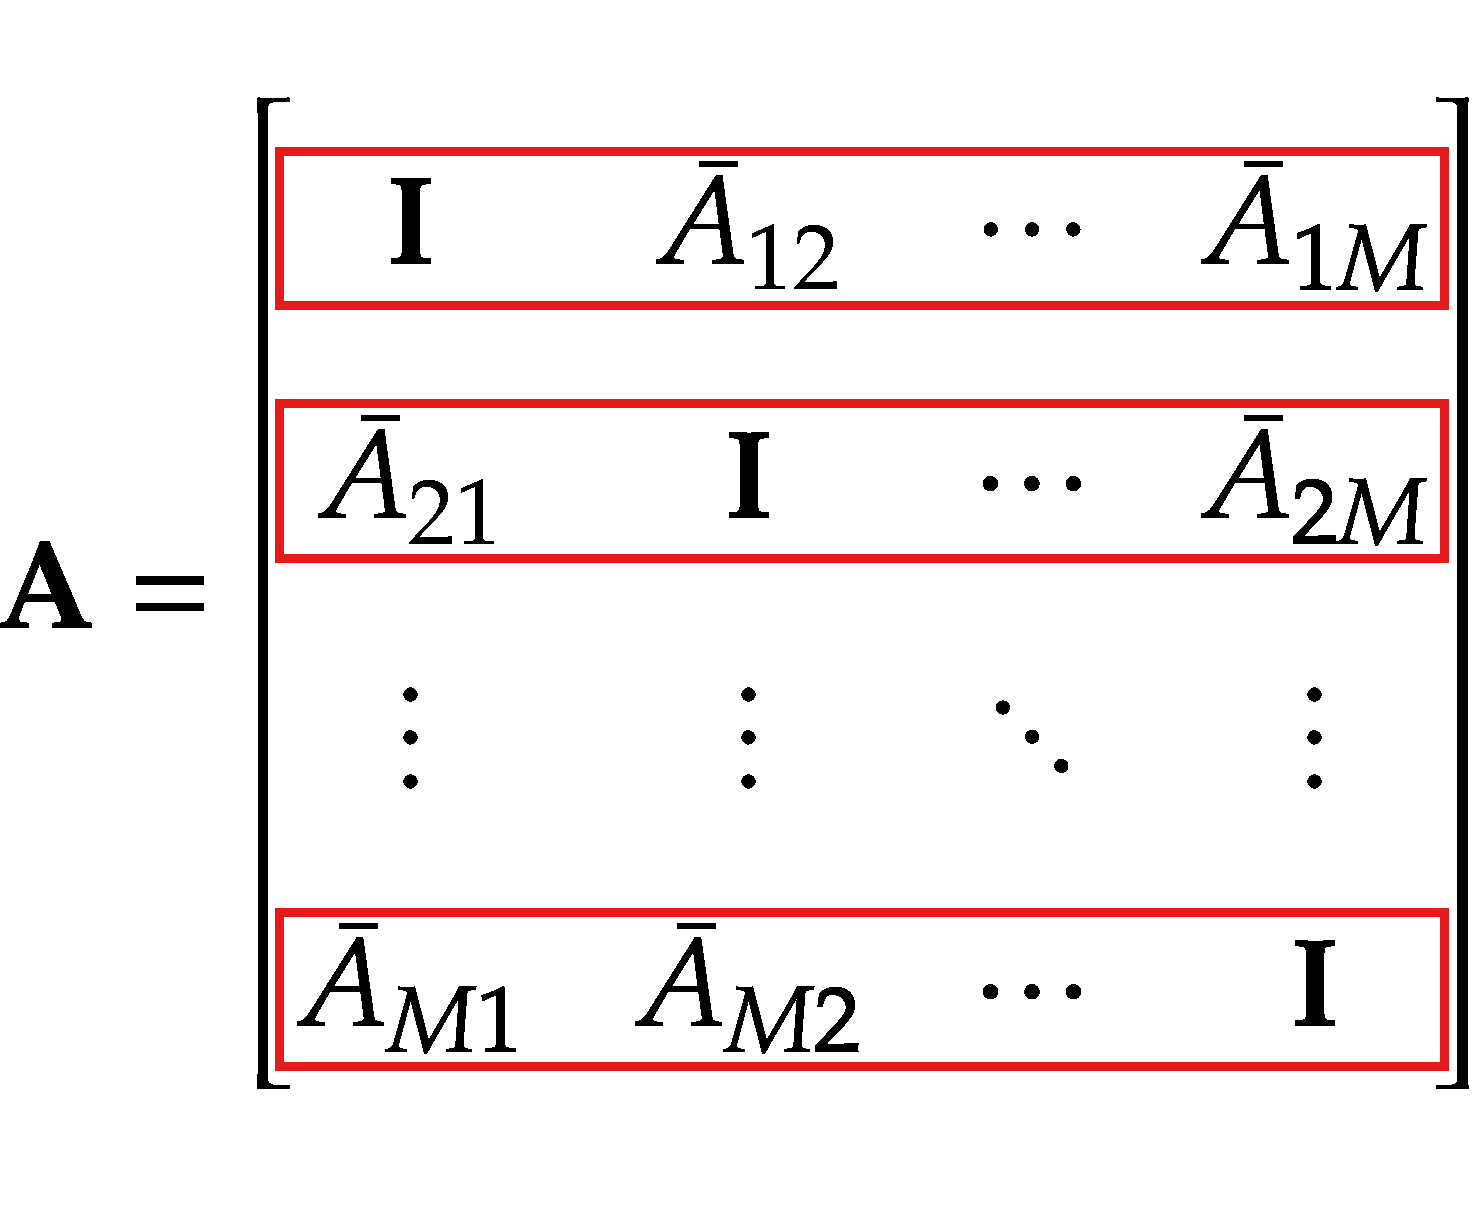
\includegraphics[width=\textwidth]{img/thread_block1D.pdf}
    \caption{1D}\label{fig:thread_block_1D}
  \end{subfigure}
  \begin{subfigure}[h]{0.33\textwidth}
    \centering
    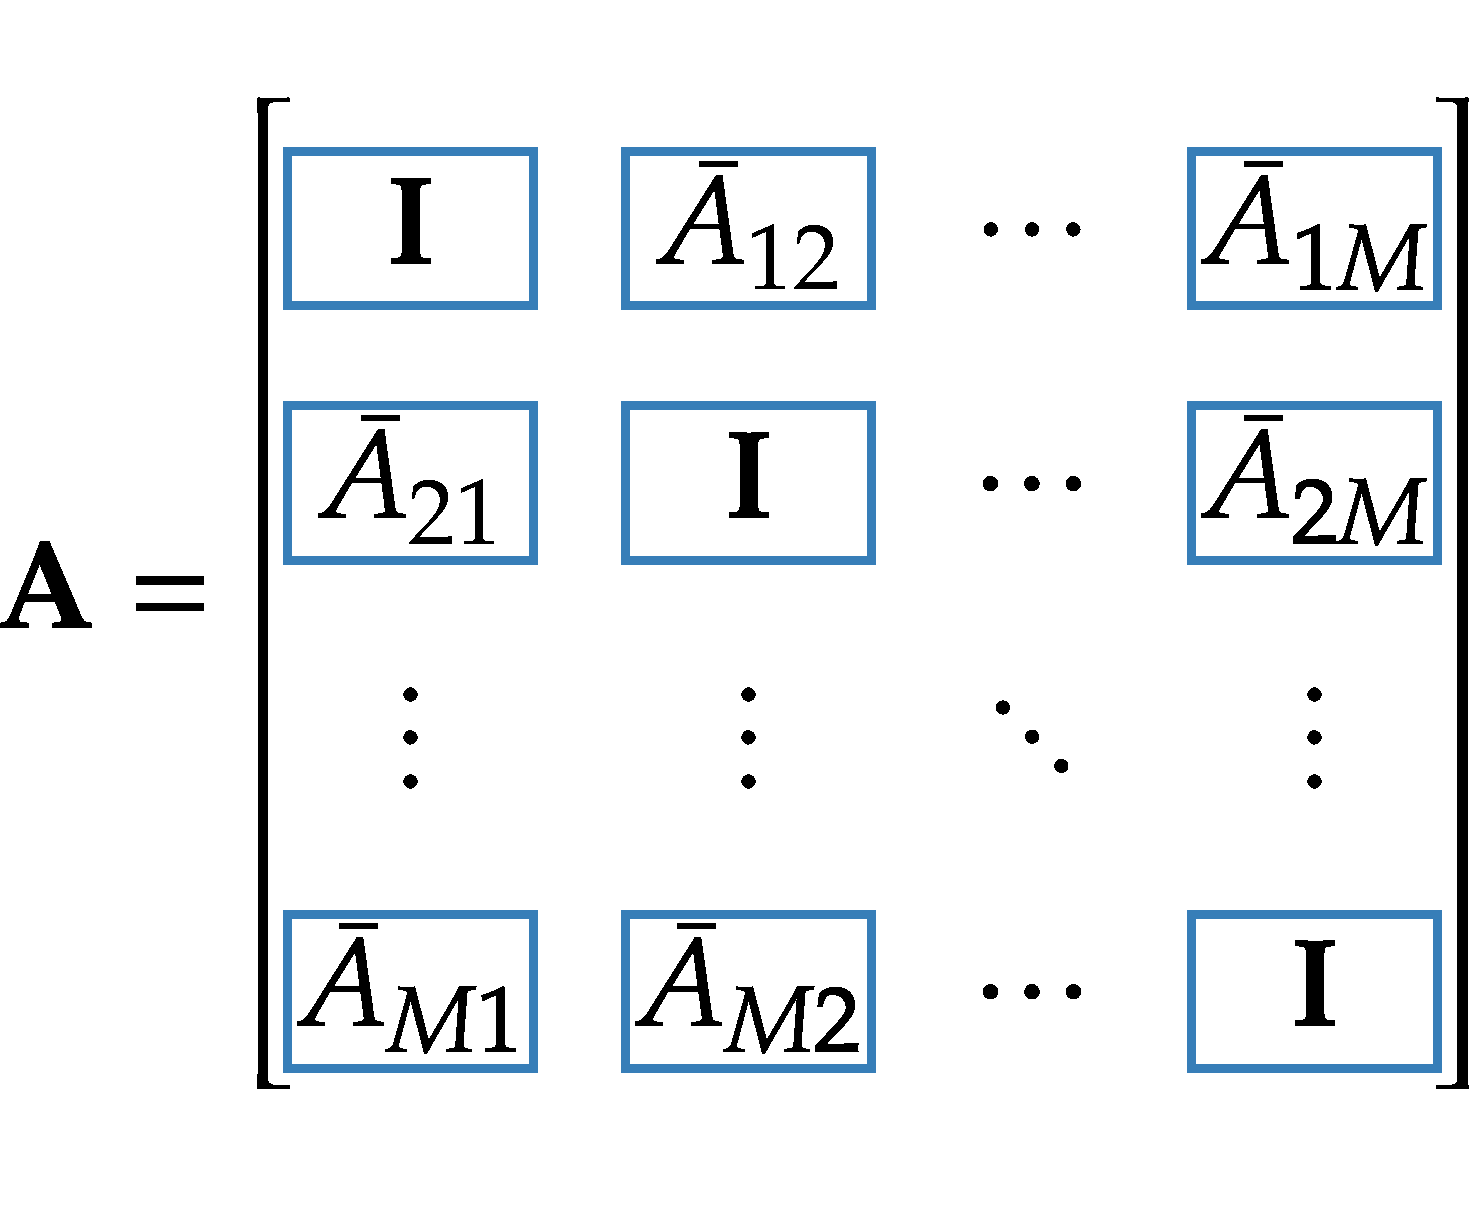
\includegraphics[width=\textwidth]{img/thread_block2D.pdf}
    \caption{2D}\label{fig:thread_block_2D}
  \end{subfigure}
  \caption{Illustration of 1D and 2D thread block dimension using simulation system matrix.}
  \label{fig:thread_block}
\end{figure}

It is not clear, how exactly the performance is affected by each decision for the thread block dimension. Only trial-and-error benchmarking combined with metrics from CUDA can find the optimal setting for the specific algorithm. We will later show in section~\ref{subsec:bench_thread_block}, that for our GPU implementation the two-dimensional approach is the most efficient one.

\section{OpenMP}

The goal of this thesis is to implement a high performance rigid fiber simulation on the GPU using CUDA. In order to better understand to what degree this goal was achieved, it is crucial to have a comparison. The original serial implementation is not an ideal candidate as it does differ in a number of ways. First of all, it is purely serial and doesn't take advantage of todays multicore CPUs. Furthermore, it was implemented in double precision and because of arbitrary restrictions NVIDIA places on its consumer GPUs, they are only suited for single precision. That is why the CUDA implementation is strictly single precision. Finally, the primary focus of the original Fortran implementation was a correctly implemented algorithm and not performance.

For these reasons and in order to have a fairer comparison of the performance differences between the GPU and CPU implementation, a completely new and rewritten parallel CPU simulation was also implemented. For the parallelization on the CPU the OpenMP library was chosen.

After having implemented a parallel algorithm for the GPU, the conversion to the OpenMP-based CPU implementation was relatively straightforward. All optimizations done for the GPU implementation were also applied to the new CPU code when applicable. In order to parallelize the BLAS functions required for the linear solver the already included OpenBLAS library was chosen. OpenBLAS is an open-source and highly optimized library and automatically parallelizes BLAS functions using pthreads across all available CPU cores. In contrast to the GPU implementation, the OpenMP version is only parallelized in one-dimension. This means that each core calculates the interactions for one fiber with all other fibers or put differently all matrix rows belong to one fiber. As the underlying number of independent threads is much lower on CPUs, different parallelization dimensions didn't have an impact during testing.

The end results of the practical implementation for this thesis is a highly optimized CUDA implementation for NVIDIA GPUs and additionally a parallelized and optimized Fortran OpenMP implementation for CPUs. The next chapter will now look at a number of performance metrics and compare them between the GPU and CPU.


\chapter{Benchmarks}
\label{cha:benchmarks}

The previous chapter introduced the parallel implementation of the numerical algorithm using NVIDIA's CUDA framework. It presented a practical overview of the GPU implementation and discussed various strategies for optimizing the algorithm.

In this chapter we will present a number of benchmark tests. The main goal of the benchmarks is to measure the performance of the GPU implementation and compare it to the performance of the OpenMP-based CPU implementation. In addition to the comparison between the two different implementations, benchmark tests are also performed to investigate the different approaches for optimizing the code presented in the previous chapter.

\section{Methodology}

The methodology used for the benchmark suite is the same for all presented benchmarks. This ensures comparable results and the fairest comparison possible. A brief overview of the hardware and benchmark scheme used are described in the next sections.

\subsection{Hardware}

All benchmarks are run on the same workstation with specifications listed in Tab.~\ref{tab:workstation}. These hardware components can be considered a balanced system. This is done to come as close as possible to a fair comparison between the CPU and GPU, as comparing a high-end CPU against a low-end GPU would only be of limited value.

\begin{table}[!htbp]
  \begin{center}
    \begin{tabulary}{0.7\textwidth}{LL}
      \toprule
      \multicolumn{2}{c}{Workstation} \\
      \midrule
      Processor & Intel Core i7 4770 \\
      Graphics & NVIDIA GTX 970 4GB \\
      RAM & 16GB DDR3 \\
      Operating System & Ubuntu Linux 12.04 LTS \\
      CUDA Driver & CUDA 6.5.16 \\
      \bottomrule
    \end{tabulary}
  \end{center}
  \caption{Benchmark hardware specification.}
  \label{tab:workstation}
\end{table}

The Intel Core i7 4770 processor is an 4-Core CPU based on Intel's Haswell Architecture. With its 8 parallel threads and $3.4$ GHz it was one of the top-of-line processor from 2013/14 and is currently still available for around $300\$$. The NVIDIA GTX 970 4GB is part of NVIDIA newest lineup of graphics cards based on the Maxwell Architecture. The main advantage of these new cards is the large memory of $4$ GB allowing for larger simulations. With a current price of slightly above $300\$$ it fills the middle price class for all Maxwell cards. Overall this can be considered to be a balanced system.

\subsection{Benchmark scheme}
\label{subsec:benchmark_scheme}

In order to generate statistically significant and reproducible execution times, all benchmarks tests for both the CPU and GPU implementation uses exactly the same run-scheme.

For each benchmark run we start with a configuration of M fibers randomly distributed in space. In order to exclude configurations where fibers overlap and/or intersect, the random process is modified such that there always is a fixed minimum distance between two fibers. Furthermore, in order to ensure a fair comparison between e.g. different linear solvers, the average distance between fibers are kept fixed for all runs independently of the number of fibers. As will be shown in Sec.~\ref{subsec:example_concentration_gmres}, the number of iterations of the iterative solvers depend on the average distance between the fibers. As the average distance become smaller, the condition number of the matrix increases and more iterations are needed for the iterative solver to converge. Thus by keeping the average distance between the fibers fixed, we minimize the influence of the number of iterations in the iterative solver on the execution time.

Using the semi-random fiber configuration, the simulation is run for 10 time steps. To avoid remaining outliers in the configuration potentially causing variations in the timings the first time step is excluded. The first time step is thus used as a simple warmup step for the simulation. So, the final average time for each run is measured using the final $9$ time steps.

To measure how the execution time depends on the number of fibers in the simulation, all tests are run with varying number of fibers starting from $100$ fibers up to $2000$ fibers using an increment of $100$.

In addition, every run is repeated a number of times where each run uses a new random fiber configuration. The final execution time is computed as the average time over the total number of runs. The execution time is measured using the built-in CUDA timing events for the GPU implementation and the Fortran \emph{SYSTEM\_CLOCK} function for the CPU implementation.

To further improve the statistical significance of the result the benchmark scheme dynamically adjusts the number of runs performed for each test. If the relative standard error (RSE) of the measured timings collected is too high after a minimum number of runs, more runs are scheduled. This repeats until the relative standard error falls below $20\%$ and reliable timings have been obtained.  The algorithm for producing the benchmark results is illustrated using pseudocode in Listing~\ref{lst:pseudo_benchmark}. 

\begin{listing}[!htbp]
  \centering
  \inputminted[mathescape,
    linenos,
    numbersep=5pt,
    fontsize=\footnotesize,
    frame=lines,
    framesep=2mm]{c}{lst/benchmark_scheme.lst}
  \caption{Pseudocode for benchmark scheme.}
  \label{lst:pseudo_benchmark}
\end{listing}

\section{Optimizations}
\label{sec:bench_optimization}

We now look at the performance results for the different optimizations strategies previously outlined in Sec.~\ref{sec:parallel_optimizations}. Where applicable, the results will be compared between the OpenMP and the CUDA version of the algorithm.

\subsection{Numeric vs. Analytic Integration}
\label{subsec:bench_numeric_vs_analytic}

The first benchmark tests the performance of the two different approaches to compute the inner integral in Eqn.~\eqref{eq:inner_integral}. It can be solved either numerically or analytically. Fig.~\ref{fig:openmp_num_vs_anal} illustrates the performance timings for the \emph{Assemble System} step of the parallel OpenMP version. Inline with the observations made by the authors of the original serial implementation,~\cite{Tornberg2006}, analytical integration is always faster to use than numerical integration.
\begin{figure}[!htbp]
  \centering
  \begin{tikzpicture}
    \begin{axis}[
	width=.9\textwidth,
      xlabel={Number of fibers},
      ylabel={Execution time (sec)},
      enlarge y limits=true,
      enlarge x limits=true,
      unbounded coords=discard,
      xmode=log,
      ymode=log,
      grid=major,
      ]
      \addplot[color=set11,mark=*,mark options={fill=white}, very thick] table[x=X,y=ASSEMBLE_SYSTEM] {benchmarks/openmp_direct_numerical.csv};
      \addplot[color=set12,mark=square*,mark options={fill=white}, very thick] table[x=X,y=ASSEMBLE_SYSTEM] {benchmarks/openmp_direct_analytical.csv};

      \legend{Numerical, Analytical}
    \end{axis}
  \end{tikzpicture}
  \caption[Benchmark computing inner integral on CPU.]{Benchmark comparing numerical and analytical integration of the inner integral in Eqn.~\eqref{eq:inner_integral} using OpenMP.}
  \label{fig:openmp_num_vs_anal}
\end{figure}

In contrast to the expected and obtained results using the OpenMP implementation, the CUDA implementation shows a different picture. When we look at the corresponding graph for the CUDA implementation in Fig.~\ref{fig:cuda_num_vs_anal}, we observe that the results are reversed. Numerical integration outperforms the analytical integration by a large margin that even increases with the number of fibers.

\begin{figure}[!htbp]
  \centering
  \begin{tikzpicture}
    \begin{axis}[
	width=.9\textwidth,
      xlabel={Number of fibers},
      ylabel={Execution time (sec)},
      enlarge y limits=true,
      enlarge x limits=true,
      unbounded coords=discard,
      xmode=log,
      ymode=log,
      grid=major,
      ]
      \addplot[color=set11,mark=*,mark options={fill=white}, very thick] table[x=X,y=assemble_system] {benchmarks/cuda_bicgstab_numerical_2D.csv};
      \addplot[color=set12,mark=square*,mark options={fill=white}, very thick] table[x=X,y=assemble_system] {benchmarks/cuda_bicgstab_analytical_2D.csv};

      \legend{Numerical, Analytical}
    \end{axis}
  \end{tikzpicture}
  \caption[Benchmark computing inner integral on GPU.]{Benchmark comparing numerical and analytical integration of the inner integral in Eqn.~\eqref{eq:inner_integral} using CUDA.}
  \label{fig:cuda_num_vs_anal}
\end{figure}

The reason for this result lies in the scheduling and execution of work on the GPU. All code inside a thread block (more precisely a warp) is always executed in lockstep. This means that each line of code is executed for each thread in parallel. However, if the code encounters a branch in the execution path, like a simple \emph{if} statement, the threads diverge. First, all threads for which the condition is true are executed while the other threads have to wait. Then all threads for which the condition is false are executed while the others are not used. Finally, after all divergent code paths have been executed the code continues in lockstep. This issue is referred to as branch divergence and should be avoided as much as possible when writing parallel GPU Code,~\cite{CudaBestPracticeGuide}.

To confirm that branch divergence is the reason for the slowdown of the analytic integration version of the GPU implementation we look at the metrics of the CUDA profiler \emph{nvprof}. The metric \emph{Warp Execution Efficency} shows the ratio of the average active threads per warp to the maximum number of threads per warp. The metrics for both the numerical and analytical integration can be seen in Tab.~\ref{tab:branch_divergence}.

\begin{table}[!htbp]
  \begin{center}
    \begin{tabulary}{0.7\textwidth}{LR}
      \toprule
      Algorithm & warp\_execution\_efficiency \\
      \midrule
      Numerical & $99.01\%$ \\
      Analytical & $53.79\%$ \\
      \bottomrule
    \end{tabulary}
  \end{center}
  \caption[Warp Execution Efficiency of Numerical vs. Analytical Integration.]{CUDA performance metric \emph{Warp Exection Efficiency} comparison for the numerical and analytical integration of the inner integral in Eqn.~\eqref{eq:inner_integral}.}
  \label{tab:branch_divergence}
\end{table}

On the one hand the numerical integration is almost $100\%$ efficient, which means that all warps execute in complete lockstep. The analytical integration on the other hand is only $50\%$ efficient, meaning that most of the time only half of the threads actually perform work while the other half is just waiting. This results in the observed performance difference. As already discussed in Sec.~\ref{subsec:numeric_analytic} the analytical evaluation of the inner integral potentially suffers from numerical instabilities. Closer inspection of the source code reveals that the steps taken to minimize these instabilities are responsible for the branch divergence and explains the decrease in performance on the GPU. The steps involve a simple \emph{if} statement, that switches between two code path depending on how far apart two fibers are. Unfortunately, this workaround is unavoidable to ensure numeric stability.

\subsection{Shared memory}
\label{subsec:bench_shared_memory}

Since the data transfer between the compute units and the global memory is slow, the second optimization strategy is to try to use shared memory to reduce the amount of data that has to be transferred. For this each Streaming Multiprocessor (SM) has a small amount of locally shared memory. This memory can be accessed from all threads on the SM. If data can be shared, it only has to be transferred from global to shared memory once. Afterwards, in can be accessed from the faster local memory.

During testing and benchmarking the shared memory implementation of the \emph{Assemble System} step described in Sec.~\ref{subsec:shared_memory}, showed no effect on the performance. Even though data can theoretically be shared among different threads it does not result in shorter execution times.

The reason for this is that the \emph{Assemble System} step is compute bound and not memory bound. This means that the time it takes to execute the computations, e.g. evaluating the integrals, takes substantially longer than reading and writing to global memory. This can be explained by looking at the two-dimensional thread block version, where each kernel is responsible for a pair of fibers. Each kernel only needs to read $4$ vectors from global memory, the position and orientation of both fibers. Assuming single precision this is a total of just $4 * 3 * 4~\text{bytes} = 48~\text{bytes}$ per kernel invocation.

While waiting for this data from global memory, CUDA is able to quickly switch between different sets of threads and continue the computation there. Thus the only waiting time occurs when the very first set of data has to be loaded. Once the first amount of data has arrived, computations can be performed using it. While the long running computations are executed, other threads can start issuing data loading requests. When the first computation is done and the next set of threads is executed, the data has already been read from memory. As there was no advantage in using shared memory in the compute bound \emph{Assemble System} step, we opted for the simpler implementation without it in all subsequent simulations.

\subsection{Thread block dimension}
\label{subsec:bench_thread_block}

The final optimization strategy studied is the Thread Block Dimension on the GPU. Choosing the best option is a trade-off between the resources used and the overhead caused by an increased amount of memory writes to the same location. Writing to the same memory location from different threads would result in undefined behavior and avoiding this requires the usage of potentially slow atomic functions.

\begin{figure}[!htbp]
  \centering
  \begin{tikzpicture}
    \begin{axis}[
      xlabel={Number of fibers},
      ylabel={Execution time (sec)},
      enlarge y limits=true,
      enlarge x limits=true,
      unbounded coords=discard,
      xmode=log,
      ymode=log,
      grid=major,
      ]
      \addplot[color=set11,mark=*,mark options={fill=white}, very thick] table[x=X,y=assemble_system] {benchmarks/cuda_magma_numerical_1D.csv};
      \addplot[color=set12,mark=square*,mark options={fill=white}, very thick] table[x=X,y=assemble_system] {benchmarks/cuda_magma_numerical_2D.csv};
      \addplot[color=set13,mark=triangle*,mark options={fill=white}, very thick] table[x=X,y=assemble_system] {benchmarks/cuda_magma_numerical_3D.csv};

      \legend{1D, 2D, 3D}
    \end{axis}
  \end{tikzpicture}
  \caption[Benchmarking thread block dimensions.]{Benchmark comparing different parallelization options of the \emph{Assemble System} step using thread block dimensions as described in Sec.~\ref{subsec:parallel_thread_block}. }
  \label{fig:bench_cuda_thread_blocks}
\end{figure}

The results in Fig.~\ref{fig:bench_cuda_thread_blocks} indicate that the best option for this particular GPU is a two-dimensional thread block. The three-dimensional thread block is always slower and the performance gap grows with the number of fibers. The reason for this performance gap is the increased usage of atomics in the three-dimensional case. The overall usage of atomic functions can be inspected with the NVIDIA profiler \emph{nvprof} and the profiling metric \emph{Atomic Transactions}. This metric simply counts the total number of atomic transactions performed when atomic functions are used. Tab.~\ref{tab:atomic_transactions} lists the \emph{Atomic Transactions} counts for both the two-dimensional and three-dimensional thread block implementation running an example with $2000$ fibers. The required \emph{Atomic Transactions} in the three-dimensional case are almost two times larger than for the two-dimensional case. These additional transactions incur a performance penalty, because they serialize the access to memory and threads have to wait while other threads finish writing to memory.

\begin{table}[!htbp]
  \begin{center}
    \begin{tabulary}{0.7\textwidth}{LR}
      \toprule
      Algorithm & atomic\_transactions \\
      \midrule
      2D & $1,269,325$ \\
      3D & $2,350,670$ \\
      \bottomrule
    \end{tabulary}
  \end{center}
  \caption[Atomic transactions of 2D vs. 3D thread block dimensions.]{CUDA performance metric \emph{Atomic transactions} comparison for the 2D and 3D thread block dimensions parallelization of the \emph{Assemble System} step.}
  \label{tab:atomic_transactions}
\end{table}

Fig.~\ref{fig:bench_cuda_thread_blocks} also shows that the one-dimensional approach is slower than both the two-dimensional and three-dimensional approach. However, it appears to scale linearly whereas the other two scale quadratically with the number of fibers. It can already be observed that the performance of the one-dimensional thread block becomes faster than the three-dimensional thread block for close to $2000$ fibers. Unfortunately, the hardware of the workstation does not have enough memory to simulate more fibers, allowing the one-dimensional approach to overtake the two-dimensional approach. Thus at least for our simulation we always use the two-dimensional approach.

\section{Linear solvers}
\label{sec:bench_linear_solvers}

Next we compare the performance for different linear solvers. The time required for solving the linear system can be a very large part of the overall runtime, depending choice of solver and the fiber configuration as discussed in Sec.~\ref{sec:algorithm_summary}. It is therefore very important to find the optimal solver in order to arrive at the best performing algorithm overall. We explore both direct and iterative solvers.

\subsection{Direct solver vs iterative solver on CPU}
On the CPU side we use the direct solver provided by the fully parallelized OpenBLAS library. For GMRES we use the single precision Fortran implementation from Frayssé et al.,~\cite{Fraysse2003}, which takes extensive advantage of the underlying BLAS functions parallelized by OpenBLAS. 

If we compare the execution time when using GMRES to using a direct solver, we observe that GMRES is faster by a wide margin, see Fig.~\ref{fig:bench_openmp_solvers}. This was also observed in the original serial version of the code,~\cite{Tornberg2006}.

\begin{figure}[!htbp]
  \centering
  \begin{tikzpicture}
    \begin{axis}[
      xlabel={Number of fibers},
      ylabel={Execution time (sec)},
      enlarge y limits=true,
      enlarge x limits=true,
      unbounded coords=discard,
      xmode=log,
      ymode=log,
      grid=major,
      ]
      \addplot[color=set11,mark=*,mark options={fill=white}, very thick] table[x=X,y=SOLVE_SYSTEM] {benchmarks/openmp_direct_numerical.csv};
      \addplot[color=set12,mark=square*,mark options={fill=white}, very thick] table[x=X,y=SOLVE_SYSTEM] {benchmarks/openmp_gmres_numerical.csv};

      \legend{Direct Solver, GMRES}
    \end{axis}
  \end{tikzpicture}
  \caption[Benchmark linear solvers on CPU.]{Benchmarking comparing linear solvers on the CPU. The direct solver is provided by OpenBLAS,~\cite{OpenBLAS}, and iterative GMRES solver by Frayssé et al.,~\cite{Fraysse2003}.}
  \label{fig:bench_openmp_solvers}
\end{figure}

From an advantage of just ${\sim}40×$ for $1000$ fibers this increases to $300×$ for the maximum number of $2000$ fibers. As expected we can also see in Fig~\ref{fig:bench_openmp_solvers} that GMRES clearly scales better with the number of fibers than the direct solver.

\subsection{Fiber concentration effect on GMRES iterations}
\label{subsec:example_concentration_gmres}

During the initial benchmark tests we observed large differences in the execution time for different fiber configurations when using GMRES. The reason for this was that for some runs, especially for a high concentration of fibers, GMRES required a large number of iterations to converge.

When the fiber concentration increases, the average distance between the fibers decreases. To investigate how the number of GMRES iterations depend on the concentration of fibers, we perform a number of runs where the average pair-wise distance between the fibers varies from $0.01$ to $40$.

\begin{figure}[!htbp]
  \centering
  \begin{tikzpicture}
    \begin{axis}[
      xlabel={Concentration},
      ylabel={GMRES iterations},
      width={0.8\textwidth},
      unbounded coords=discard,
      xmode=log,
      ymode=log,
      grid=major,
      xmin=0.01,xmax=100,
      ymin=0.1,ymax=1000,
      ]

      \addplot[color=set11, mark=*,mark options={fill=white}, very thick] table[x=Concentration,y=Average,col sep=comma] {charts/concentration_gmres.csv};

    \end{axis}
  \end{tikzpicture}
  \caption[Effect of fiber concentration on GMRES iterations.]{Effect of fiber concentration on GMRES iterations. The number of GMRES iterations increases dramatically when the distance between the fibers is small.}
  \label{fig:concentration_gmres}
\end{figure}

In Fig.~\ref{fig:concentration_gmres} the result is presented. We see that for a decrease in the pair-wise distance, the number of iterations increases quite rapidly. To find the reason for this we have to look at Eqn.~\eqref{eq:inner_integral} which forms the basis for the entries in the matrix. When evaluating the integral the Greens function $\mathbf{G}(\mathbf{R})$ defined in Eqn.~\eqref{eq:green_function} has to be computed. Since $\mathbf{G}(\mathbf{R}) \sim 1/\mathbf{R}$ where $\mathbf{R}$ is given by the distance between fibers, some of the entries in the matrix become very large when the distance is small. The consequence is a growth in the condition number of the matrix and thus an increase in the number of GMRES iterations is required for convergence. This is the reason why we keep the concentration of fibers fixed for all benchmark runs, as described in Sec.~\ref{subsec:benchmark_scheme}.

The result presented above is also important to keep in mind when performing long running fiber simulations. Here, the probability that any two fibers get close to each other is very high. If this is the case, solving the system by GMRES will take longer than expected. In practice it might be more beneficial to switch to the direct solver as it has a predictable runtime. This is especially true using the GPU implementation as the difference in execution time between direct and iterative solver is relatively small. This will be discussed further in the next section.

\subsection{Direct solver vs. iterative solver on GPU}

We will now look at the performance of the direct solver compared to the iterative solvers on the GPU. We use a direct solver provided by the MAGMA library and the iterative solvers, BiCGStab and GMRES, from the ViennaCL library. The benchmark results are illustrated in Fig.~\ref{fig:bench_cuda_solvers}.

\begin{figure}[!htbp]
  \centering
  \begin{tikzpicture}
    \begin{axis}[
      xlabel={Number of fibers},
      ylabel={Execution time (sec)},
      enlarge y limits=true,
      enlarge x limits=true,
      unbounded coords=discard,
      xmode=log,
      ymode=log,
      grid=major,
      ]
      \addplot[color=set11,mark=*,mark options={fill=white}, very thick] table[x=X,y=solve_system] {benchmarks/cuda_magma_numerical_2D.csv};
      \addplot[color=set12,mark=square*,mark options={fill=white}, very thick] table[x=X,y=solve_system] {benchmarks/cuda_bicgstab_numerical_2D.csv};
      \addplot[color=set13,mark=triangle*,mark options={fill=white}, very thick] table[x=X,y=solve_system] {benchmarks/cuda_gmres_numerical_2D.csv};

      \legend{Direct Solver, BiCGStab, GMRES}
    \end{axis}
  \end{tikzpicture}
  \caption[Benchmark linear solvers on GPU.]{Benchmarking comparing linear solvers on the GPU. The direct solver is provided by MAGMA,~\cite{MagmaDocumentation}, and iterative solvers, BiCGStab and GMRES, by ViennaCL,~\cite{ViennaCLRupp2010}.}
  \label{fig:bench_cuda_solvers}
\end{figure}

The fact that iterative solvers are faster than a direct solver holds true also for the GPU. However, compared to the results on the CPU the difference between the performance of the direct solver and the iterative solvers is not as large. At close to $2000$ fibers the iterative solvers are only about $25×$ faster than the direct solver as compared to the result on the CPU where GMRES was $300×$ faster than the direct solver. Looking at the difference between the two iterative solvers, BiCGStab and GMRES they perform almost exactly the same. Any small differences can be attributed to small measuring uncertainties. 

Regardless of these clear results, it is always important to keep in mind, that this particular performance ratio only holds true for the specific fiber concentration which was benchmarked. For other concentrations the iterative solvers might need more iterations to find the solution and might even perform worse than the linear solver.

\section{Individual steps of the algorithm}

The next benchmark explores the relative time taken by each step of the algorithm described in Sec.~\ref{sec:algorithm_summary}~and Sec.~\ref{sec:kernels}. This yields valuable insight into the time allocation of the overall execution time, thereby helping to figure out which steps are the best ones to optimize. The results for the OpenMP implementation can be seen in Fig.~\ref{fig:bench_openmp_steps} and for the CUDA implementation in Fig.~\ref{fig:bench_cuda_steps}. On the CPU the \emph{Assemble System} and \emph{Update Velocities} steps solve the inner integral in Eqn.~\eqref{eq:inner_integral} analytically. On the GPU we use a purely numerical approach. The reason for choosing different approaches for evaluating the inner integral is to use the fastest version of the algorithm on both the CPU and GPU, see Sec.~\ref{subsec:bench_numeric_vs_analytic}.

\begin{figure}[!htbp]
  \centering
  \begin{tikzpicture}
    \begin{axis}[
      xlabel={Number of fibers},
      ylabel={Execution time (sec)},
      stack plots=y,
      ymin=0,ymax=50,
      xmin=0,xmax=2000,
      ]
      \addplot[color=set19,mark=*,mark options={fill=white}, very thick, stack plots=false] table[x=X,y=TOTAL] {benchmarks/openmp_gmres_analytical.csv};
      \addplot[color=set11,fill=set11_light,ultra thin,area style] table[x=X,y=ASSEMBLE_SYSTEM] {benchmarks/openmp_gmres_analytical.csv} \closedcycle;
      \addplot[color=set12,fill=set12_light,ultra thin,area style] table[x=X,y=SOLVE_SYSTEM]{benchmarks/openmp_gmres_analytical.csv} \closedcycle;
      \addplot[color=set13,fill=set13_light,ultra thin,area style] table[x=X,y=UPDATE_VELOCITIES] {benchmarks/openmp_gmres_analytical.csv} \closedcycle;
      \addplot[color=set14,fill=set14_light,ultra thin,area style] table[x=X,y=UPDATE_FIBERS] {benchmarks/openmp_gmres_analytical.csv} \closedcycle;

      \legend{Total, Assemble System, Solve System, Update Velocities, Update Fibers}
    \end{axis}
  \end{tikzpicture}
  \caption[Benchmark individual steps on CPU.]{Benchmark comparing the execution for each individual step of the algorithm using the OpenMP-based CPU implementation.}
  \label{fig:bench_openmp_steps}
\end{figure}

The results for the OpenMP implementation, Fig.~\ref{fig:bench_openmp_steps}, show that for $2000$ fibers the \emph{Assemble System} step is responsible for $78\%$ and the \emph{Update Velocities} step for $21\%$ of the overall time. The two other steps \emph{Solve System} and \emph{Update Fibers} barely register with just $1\%$. However, as discussed in the previous Sec.~\ref{sec:bench_linear_solvers} this only holds true for sufficiently low concentrations of fibers.

\begin{figure}[!htbp]
  \centering
  \begin{tikzpicture}
    \begin{axis}[
      xlabel={Number of fibers},
      ylabel={Simulation time (sec)},
      stack plots=y,
      ymin=0,ymax=1.4,
      xmin=0,xmax=2000,
      ]
      \addplot[color=set19,mark=*,mark options={fill=white}, very thick, stack plots=false] table[x=X,y=total] {benchmarks/cuda_gmres_numerical_2D.csv};
      \addplot[color=set11,fill=set11_light,ultra thin,area style] table[x=X,y=assemble_system] {benchmarks/cuda_gmres_numerical_2D.csv} \closedcycle;
      \addplot[color=set12,fill=set12_light,ultra thin,area style] table[x=X,y=solve_system]{benchmarks/cuda_gmres_numerical_2D.csv} \closedcycle;
      \addplot[color=set13,fill=set13_light,ultra thin,area style] table[x=X,y=update_velocities] {benchmarks/cuda_gmres_numerical_2D.csv} \closedcycle;
      \addplot[color=set14,fill=set14_light,ultra thin,area style] table[x=X,y=update_fibers] {benchmarks/cuda_gmres_numerical_2D.csv} \closedcycle;

      \legend{Total, Assemble System, Solve System, Update Velocities, Update Fibers}
    \end{axis}
  \end{tikzpicture}
  \caption[Benchmark individual steps on GPU.]{Benchmark comparing the execution for each individual step of the algorithm using the CUDA-based GPU implementation.}
  \label{fig:bench_cuda_steps}
\end{figure}

For the CUDA implementation, Fig.~\ref{fig:bench_cuda_steps} shows that the \emph{Assemble System} step remains the largest block with $72\%$ of the time. However, now the \emph{Solve System} step takes $20\%$ of the time and \emph{Update Velocites} drops to just $7\%$. The \emph{Update Fibers} step is also negligible here with below $1\%$.

This difference between the CPU and GPU implementation in the relative time between the steps can be attributed to the comparatively slow GMRES implementation on the GPU. In absolute terms for $2000$ fibers both the CPU and GPU take ${\sim}0.25$ seconds for solving the system. But, when transferring the same relative distribution from the CPU to GPU this makes the GPU GMRES implementation $40×$ too slow. The other steps all perform relatively better.

The reason for this most likely lies in the non-optimized code for the GMRES solver in ViennaCL. The authors openly state that the major goal for their library is easy of use and not pure performance,~\cite{ViennaCLRupp2010}. The parallel BLAS functions from OpenBLAS on the other hand have been highly optimized and tested for a long time.

This point is reinforced if we look at the same timings for the linear solvers. Here the absolute time for \emph{Solve System} step on the GPU is just ${\sim}7$ seconds compared to the ${\sim}76$ seconds on the CPU. Again transferring the relative distribution from the CPU to the GPU yields just a small factor of ${\sim}1.4×$. This illustrates that the highly optimized code of the MAGMA library performs roughly on the same level as the optimized code from OpenBLAS.

\section{GPU vs. CPU}

The final benchmark compares the CPU and GPU performance. How to make a fair comparison of the simulation performance between the CPU and GPU is a hotly debated topic in the research literature,~\cite{Gregg2011}\cite{Lee2010}. The underlying architectures of the two approaches are completely different and thus hard to compare. There are approaches where the relative performance is extrapolated from the underlying FLOPs by taking processor count, frequency and memory bandwidth into account,~\cite{Lee2010}. However, due to intricate hardware details this approach is not applicable to all scenarios. Thus in the super computing community metrics like performance-per-dollar or even performance-per-watt have become the main focus,~\cite{Kamil2008}.

Exploring this question in more detail is out of the scope of this thesis. Nevertheless we try to make a best effort to do fair comparison between the CPU and the GPU performance. In order to come as close as possible given these complexities and constraints, we use a modern CPU and GPU which can be considered a balanced system at the time of writing. Additionally, we implemented a parallel OpenMP version. It is directly based on the parallel CUDA version with the sole purpose to have as few difference between the two implementations as possible. Furthermore, the final benchmark uses the fastest possible version of the algorithms as determined by the performed benchmarks.

The results for the average time required to take a single time step is illustrated in Fig.~\ref{fig:overall}. For OpenMP the algorithm uses the analytical integration of the inner integral. For CUDA, we used the numerical integration and the thread block dimension was chosen to be 2-dimensional.

\begin{figure}[!htbp]
  \centering
  \begin{tikzpicture}
    \begin{axis}[
      xlabel={Number of fibers},
      ylabel={Execution time (sec)},
      enlarge y limits=true,
      enlarge x limits=true,
      unbounded coords=discard,
      xmode=log,
      ymode=log,
      grid=major,
      ]

      \addplot[color=set11,mark=*,mark options={fill=white}, very thick] table[x=X,y=total] {benchmarks/cuda_gmres_numerical_2D.csv};
      \addplot[color=set11_light,mark=square*,mark options={fill=white}, very thick] table[x=X,y=total] {benchmarks/cuda_magma_numerical_2D.csv};
      \addplot[color=set12,mark=triangle*,mark options={fill=white}, very thick] table[x=X,y=TOTAL] {benchmarks/openmp_gmres_analytical.csv};
      \addplot[color=set12_light,mark=diamond*,mark options={fill=white}, very thick] table[x=X,y=TOTAL] {benchmarks/openmp_direct_analytical.csv};

      \legend{CUDA GMRES, CUDA Direct, OpenMP GMRES, OpenMP Direct}
    \end{axis}
  \end{tikzpicture}
  \caption[Benchmark overall execution time.]{Benchmark comparing overall execution time for OpenMP and CUDA. Both the CPU and GPU implementation are run using the fastest algorithm as determined in Sec~\ref{sec:bench_optimization} and each implementation is tested with a direct and iterative solver. The CUDA-based GPU implementation outperforms the OpenMP-based CPU implementation by ${\sim}40×$.}
  \label{fig:overall}
\end{figure}

The required simulation time on the GPU outperforms the CPU by a wide margin. The GPU version is faster for any number of fibers that we are able to test. The speedup factors for the tested versions are listed in Tab~\ref{tab:overall_speedup}. CUDA maintains a relative performance of ${\sim}40×$. The only advantage the CPU version has is the potentially larger memory as 4GB on the GPU limits the number of fibers to roughly $2000$. So for more fibers than $2000$, OpenMP is currently the only option.

\begin{table}[!htbp]
  \begin{center}
    \begin{tabulary}{\textwidth}{lRRRR}
      \toprule
      M = 2000 & OpenMP Direct & OpenMP GMRES & CUDA Direct & CUDA GMRES \\
      \midrule
      OpenMP Direct & $1×$  & $—$   & $—$ & $—$ \\
      OpenMP GMRES  & $3×$  & $1×$  & $—$ & $—$ \\
      CUDA Direct   & $16×$ & $6×$  & $1×$ & $—$ \\
      CUDA GMRES    & $99×$ & $39×$ & $6×$ & $1×$ \\
      \bottomrule
    \end{tabulary}
  \end{center}
  \caption[Speedup factors for overall execution time.]{The speedup factors for the overall execution time of a simulation with $2000$ fibers for the CPU and GPU implementation. In case of a direct solver the GPU implementation shows a speedup of $16×$ compared to the CPU implementation. Comparing the two GMRES versions, the CUDA-based GPU implementation outperforms the OpenMP-based CPU implementation by $39×$.}
  \label{tab:overall_speedup}
\end{table}

We acknowledge that these numbers and performance increases are not necessarily fair. A different CPU and GPU combination from the one used in this thesis might perform differently. However, the relative performance should stay roughly the same. In the end, the only thing that really matters for the researcher working with rigid fibers is the time it takes to simulate large systems on the available workstation. There is no need to wait for computing time at a large computing cluster. Instead simulation can be run simply on a desktop computer allowing to rapidly iterate on the tests. The observed performance increase of $40×$ is comparable to a difference between a whole day of waiting for the simulation results and a quick $30$ minutes result. The saved time also translates directly into the ability to simulate many more fibers than before. Using the original serial implementation the largest simulation possible in a reasonable time frame where around $500$ to $800$ fibers. Now one single time step with $2000$ fibers takes at most $8$ seconds on the GPU. Therefore the implementation on the GPU and the optimizations of the simulation code is of great value to the research of rigid fiber simulations.


\chapter{Experiments}
\label{cha:experiments}

The previous chapter showed how much faster the CUDA implementation is compared to the same algorithm implemented on the CPU. This significant increase in performance allows for new experiments.

We will now perform a number of experiments to explore the numerical precision and validate the results against prior research. We begin by looking at tumbling orbits, a very delicate experiment requiring great precision. This is followed by a quick look at the effect of the fiber concentration on the required GMRES iterations to settle on the solution. Next we reproduce a very interesting physical phenomenon of letting a sphere of fibers sediment and validate our results against similar experiment by others. Furthermore, we will have a brief exploration of the effects of the number of fibers and the concentration of fibers on the sphere simulation. All experiments were run with the purely numerical, 2-dimensional CUDA algorithm  implemented in the thesis. The systems were solved using the direct solver from MAGMA in order to avoid variations in the run time.

\section{Tumbling orbits}
\label{sec:example_ring}

The first example was used to verify that the single precision GPU version is able to replicate the result of the original double precision code. For this we looked at a very simple problem where a small number of fibers are set up with perfectly symmetrical positions and orientations. All fibers are evenly distributed on a circle and aligned vertically with gravity. During the simulation the fibers begin to rotate from their vertical orientation towards the horizontal position. Afterwards, they continue rotating back into the vertical position. This motion is referred to as tumbling orbits and as long as there are no disturbances or numerical precision issues it repeat forever.

This simple but very interesting problem has also been simulated by Gustavsson and Tornberg \cite{Gustavsson2009}. Additionally an even more simplified version with only two fibers was studied both numerically and experimentally by Jung et al. \cite{Jung2006}. This example is thus ideally suited to test and verify the numerical precision of the GPU simulation. A visualization of the GPU simulation of $16$ fibers evenly distributed around a circle with a radius of $0.55$, is shown in Figure~\ref{fig:ring_simulation}.

\begin{figure}[!htbp]
  \centering
  \begin{subfigure}[h]{0.45\textwidth}
    \centering
    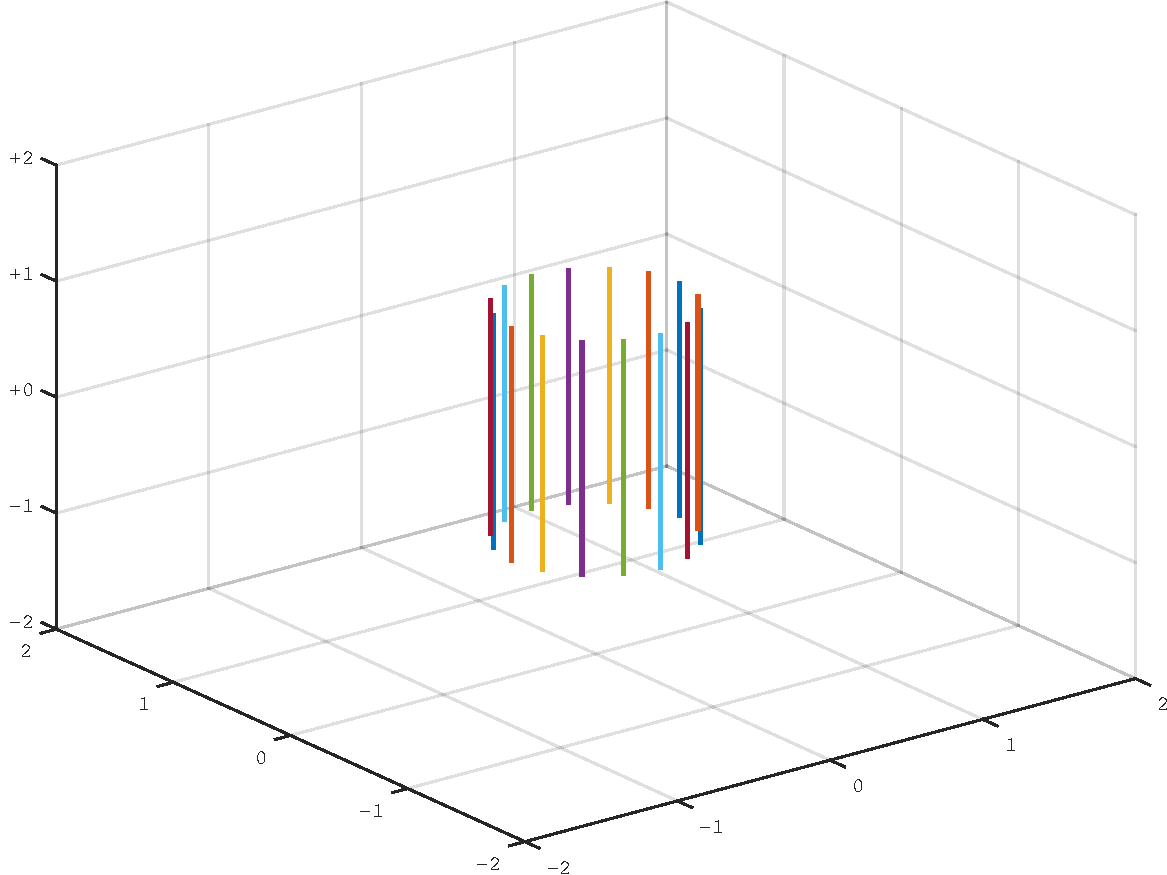
\includegraphics[width=\textwidth]{img/ring_00000.pdf}
    \caption{$t=0$}\label{fig:ring_simulation_1a}
  \end{subfigure}
  \begin{subfigure}[h]{0.45\textwidth}
    \centering
    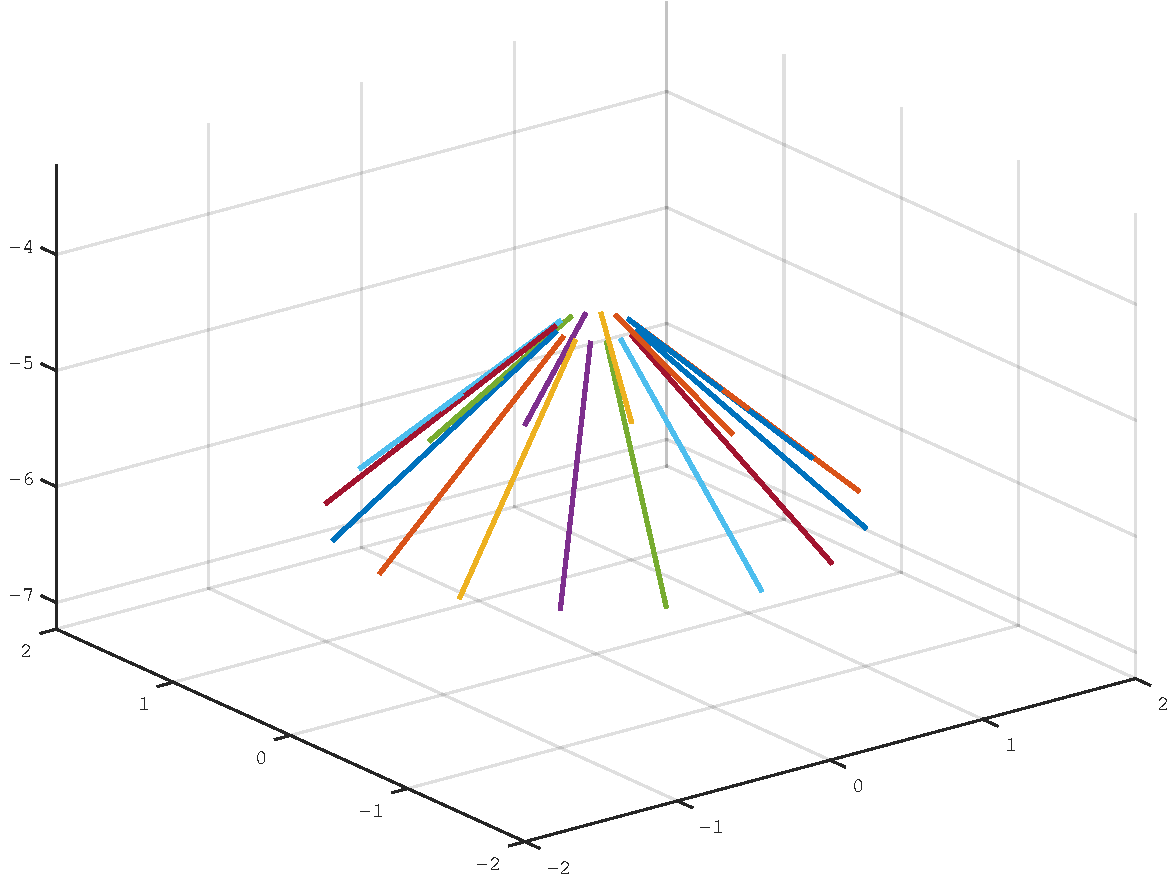
\includegraphics[width=\textwidth]{img/ring_00015.pdf}
    \caption{$t=15$}\label{fig:ring_simulation_1b}
  \end{subfigure}
  \begin{subfigure}[h]{0.45\textwidth}
    \centering
    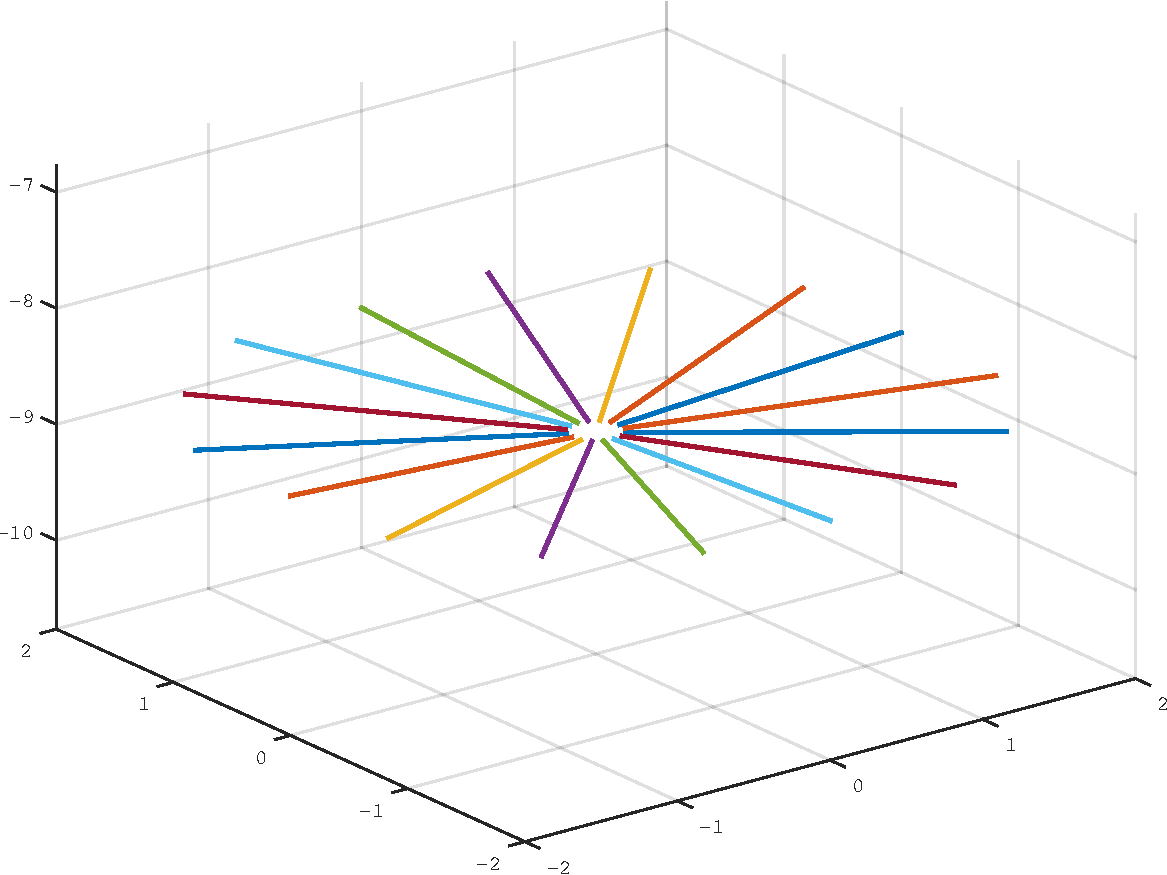
\includegraphics[width=\textwidth]{img/ring_00030.pdf}
    \caption{$t=30$}\label{fig:ring_simulation_1c}
  \end{subfigure}
  \begin{subfigure}[h]{0.45\textwidth}
    \centering
    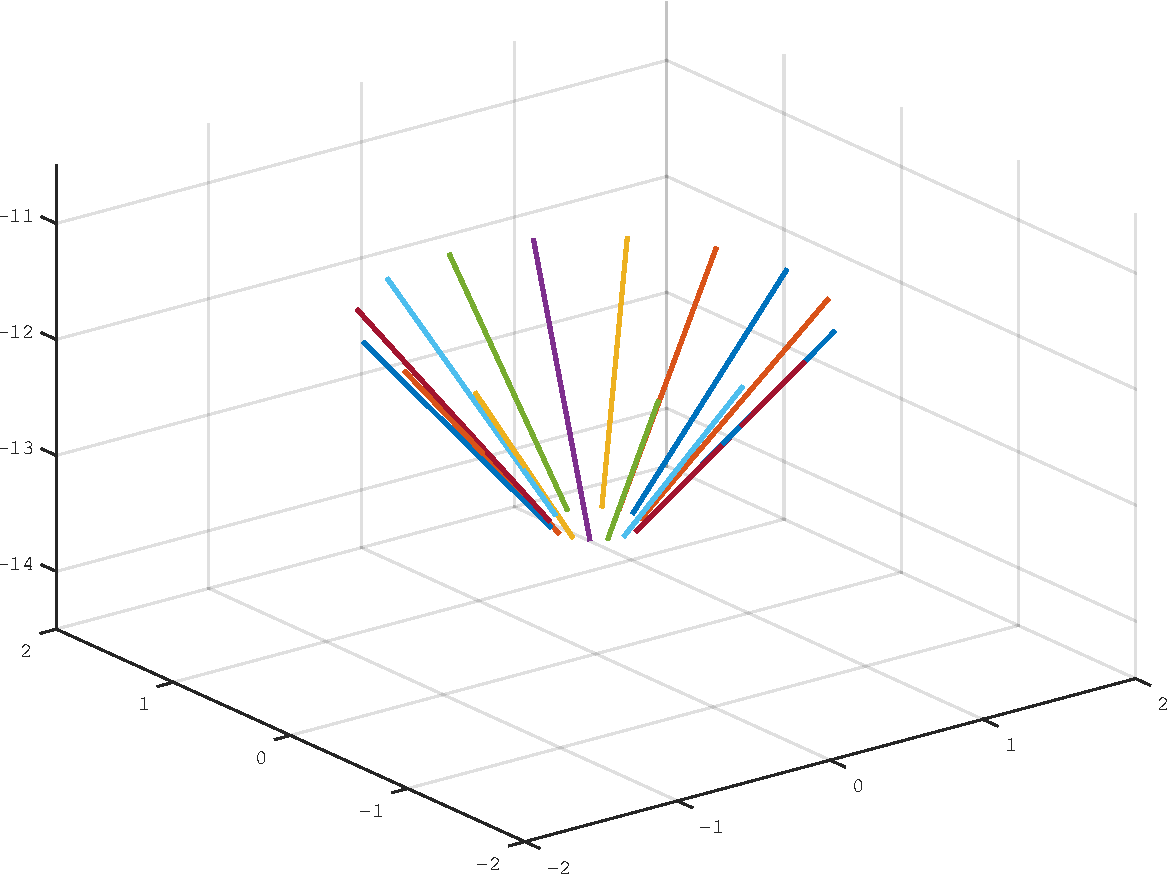
\includegraphics[width=\textwidth]{img/ring_00045.pdf}
    \caption{$t=45$}\label{fig:ring_simulation_1d}
  \end{subfigure}
  \caption{Visualization Tumbling Orbits.}
  \label{fig:ring_simulation}
\end{figure}

In order to analyze the periodic movement of the fibers we now look at the sedimentation velocity caused by gravity. In the initial setup the fibers are aligned vertically and are dropping with the maximum velocity. As they rotate into the horizontal orientation the velocity is decreasing and reaches its minimum once the fibers are perpendicular to the direction of gravity. Afterwards on their way back to vertical orientation the velocity increases again.

Figure~\ref{fig:ring_sedimentation_velocity} shows a graph of the sedimentation velocity of a single fiber over time for both the single precision GPU code and the original double precision Fortran code. As the same force acts on all fibers and they perform the same motion they all have the same sedimentation velocity. For this particular setup the maximum velocity is $~3.8$ and the minimum velocity is $~2.2$. The graphs clearly shows the periodical rotation the fiber perform. This result perfectly captures the expected result obtained from prior simulation and experiments.

\begin{figure}[!htbp]
  \centering
  \begin{tikzpicture}
    \setmathfont{FiraSans-Book.otf}
    \begin{axis}[
      title=Sedimentation Velocity,
      xlabel={timestep},
      ylabel={velocity},
      height={207pt},
      unbounded coords=discard,
      xmin=0,xmax=200,
      ymin=-4,ymax=-2,
      ]

      \addplot[color=set12, very thick] table[x=Timestep,y=Single] {charts/ring_sedimentation.csv};
      \addplot[color=set11, loosely dashed, ultra thick] table[x=Timestep,y=Double] {charts/ring_sedimentation.csv};

      \legend{Single Precision, Double Precision}
    \end{axis}
    \setmathfont{Asana-Math.otf}
  \end{tikzpicture}
  \caption{Comparison of sedimentation velocity for single- and double-precision simulation.}
  \label{fig:ring_sedimentation_velocity}
\end{figure}

\section{Fiber concentration effect on GMRES iterations}
\label{sec:example_concentration_gmres}

As alluded to in the discussion about the performance of direct solvers versus iterative solvers in section~\ref{sec:bench_linear_solvers} we will now investigate how the concentration of fibers affects the GMRES iterations. In this context the concentration of fibers refers to the average distance between each fiber and its closest neighbor. Thus we use the average minimal pair-wise distance between the fibers as a measurement of fiber concentration. Figure~\ref{fig:concentration_gmres} illustrates the number of iterations GMRS needs to solve the system for a given pair-wise distance. Please note that the x-axis as well as the y-axis are logarithmic to improve clarity.

\begin{figure}[!htbp]
  \centering
  \begin{tikzpicture}
    \setmathfont{FiraSans-Book.otf}
    \begin{axis}[
      title=Effect of fiber concentration on number of GMRES iterations,
      xlabel={concentration},
      ylabel={GMRES iterations},
      width={0.8\textwidth},
      unbounded coords=discard,
      xmode=log,
      ymode=log,
      grid=major,
      xmin=0,xmax=100,
      ymin=0,ymax=400,
      ]

      \addplot[color=set11, mark=*,mark options={fill=white}, very thick] table[x=Concentration,y=Average] {charts/concentration_gmres.csv};

    \end{axis}
    \setmathfont{Asana-Math.otf}
  \end{tikzpicture}
  \caption{Effect of fiber concentration on GMRES iterations.}
  \label{fig:concentration_gmres}
\end{figure}

We can see that for an increasing average pair-wise distance, i.e. a lower fiber concentration, the number of iterations decreases. The average iteration count for the concentration (average distance of $0.4$) we used during our benchmarks in Chapter~\ref{cha:benchmarks} lies between $3$ and $10$. However, as the average pair-wise distance decreases we observe an exponential increase in the number of iterations.

To find the reason for this we have again have to look at the integral in equation~\eqref{eq:inner_integral} which has to be solved for each fiber pair during the \emph{Assemble System} step. The required Stokeslet computations in equation~\eqref{eq:stokeslet} include the distance between the fibers in the denominator. As the distance gets very small the value of the Stokeslet becomes large. These large terms can then cause the assembled matrix to become ill-conditioned and thus increase the number of iterations GMRES requires to settle on a solution.

This result is important to keep in mind when simulating long running complex fiber configuration. Here the probability that any two fibers get close to each other is very high. If this is the case solving the system using GMRES takes longer than expected. In practice it might thus be beneficial to switch to the direct solver, as it has a predictable runtime. This is especially true because the performance difference between direct and iterative solvers on the GPU is relatively small.

\section{Sedimenting sphere}
\label{sec:example_sphere}

The next example showcases a more chaotic system with a large number of interacting fibers. This experiment is studied by several papers\cite{Metzger2007}\cite{Park2010}\cite{Bulow2015}. It is especially interesting because the observed results only occur if enough fibers are simulated. Our GPU simulation is able to efficiently handle up to $2000$ fibers and is thus ideally suited for studying this example. For the experiment $2000$ fibers are initially distributed inside a sphere with a concentration of $0.4$. Both their positions and orientations are randomly generated inside this sphere. An illustration of an example run can be seen in Figure~\ref{fig:sphere_simulation}.

\begin{figure}[!htbp]
  \centering
  \begin{subfigure}[h]{0.4\textwidth}
    \centering
    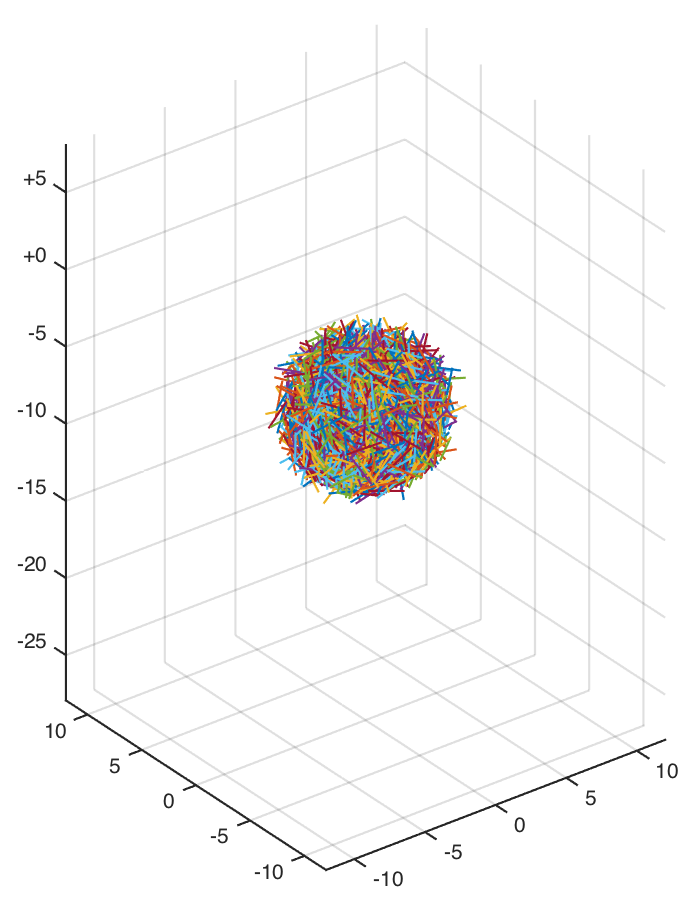
\includegraphics[width=\textwidth]{img/state_00000.pdf}
    \caption{$t=0$}\label{fig:sphere_simulation_1a}
  \end{subfigure}
  \begin{subfigure}[h]{0.4\textwidth}
    \centering
    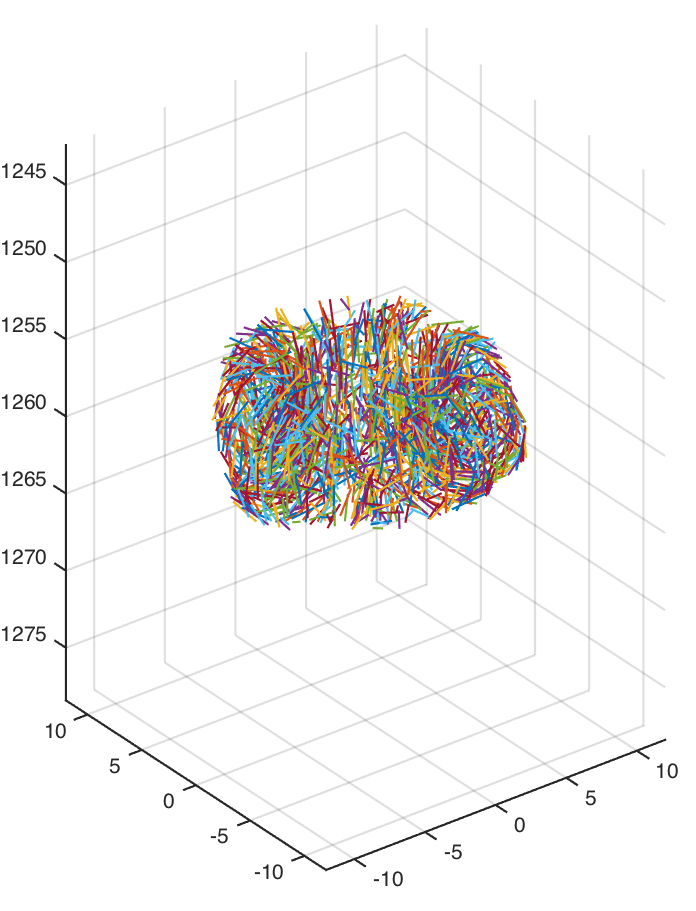
\includegraphics[width=\textwidth]{img/state_00250.pdf}
    \caption{$t=300$}\label{fig:sphere_simulation_1b}
  \end{subfigure}
  \begin{subfigure}[h]{0.4\textwidth}
    \centering
    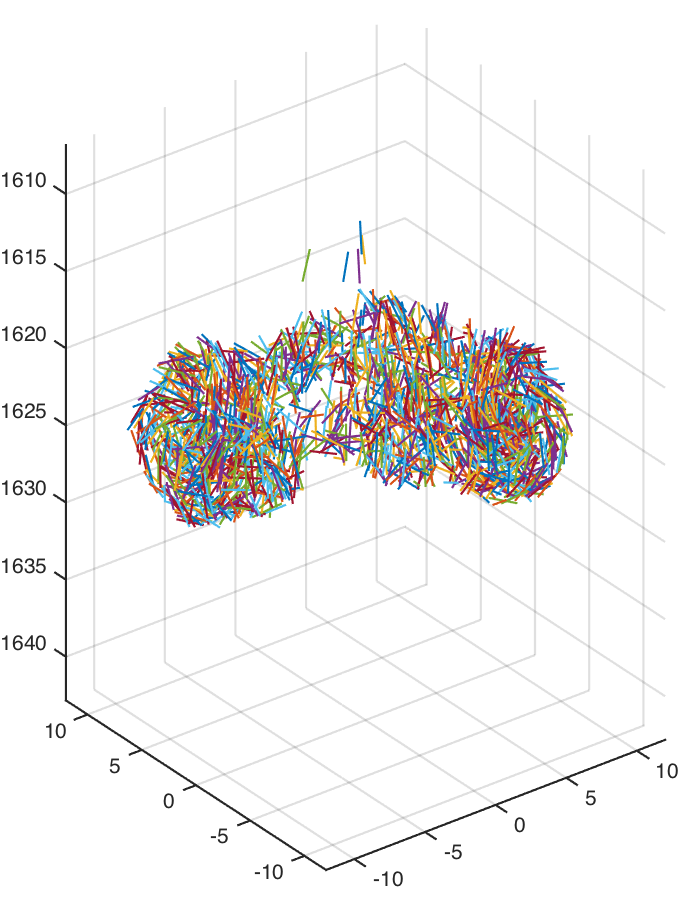
\includegraphics[width=\textwidth]{img/state_00350.pdf}
    \caption{$t=350$}\label{fig:sphere_simulation_1c}
  \end{subfigure}
  \begin{subfigure}[h]{0.4\textwidth}
    \centering
    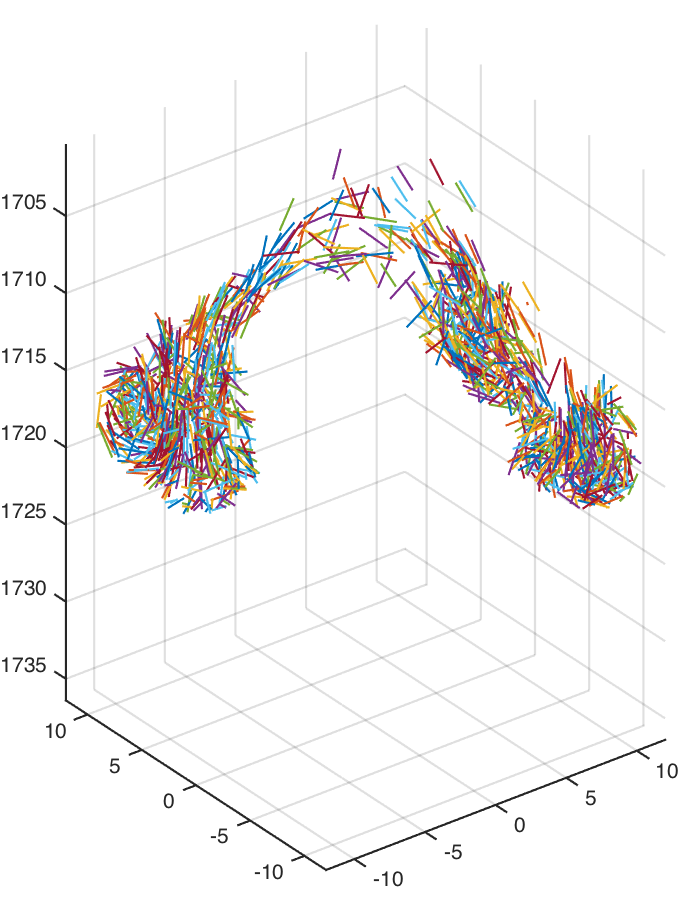
\includegraphics[width=\textwidth]{img/state_00380.pdf}
    \caption{$t=380$}\label{fig:sphere_simulation_1d}
  \end{subfigure}
  \caption{Visualization Sedimenting Sphere.}
  \label{fig:sphere_simulation}
\end{figure}

This sphere of packed fibers is then allowed to sediment due to gravity. Beginning from the spherical shape the interacting fibers slowly begin to form a continuously turning torus. Even though the behavior is more chaotic due to the large number of fibers and the random initial setup, this turning torus resembles the result for the tumbling orbits in section~\ref{sec:example_ring}.

After some time the torus breaks and the fibers are split into multiple smaller clusters. Each cluster continues to sediment separately and slowly forms its own smaller torus again. However, due to tiny variations these toruses can be harder to see.

The calculation of the presented example only takes $~7.7$ seconds with the GPU simulation. Consequently it is possible to perform the $500$ time steps of the simulation in a little bit over $1$ hour. Simulating this many fibers in such a short time will allow new research of this interesting phenomenon. One interesting research question is for example determining what influences the stability of the torus.

To begin investigating this question we first define the stability of the torus in terms of the break up time. How to determine the exact break up time of the torus is quite challenging. This problem and question was also examined by Park et al. \cite{Park2010}. They define the break up as the moment when the torus starts to bend prior to actually breaking. Additionally, they describe an algorithm that determines which fibers are part of the torus. Consequently, they compute metrics such as the remaining fibers, the radius and velocity of the sedimenting torus. Unfortunately, they don't define a metric that determines the exact break up time. Thus we came up with our own measure of the break up time based on their work.

We use the same definition for the torus as described by Park et al. \cite{Park2010}. First we compute the initial radius $R_0$ of the sphere. Then as the sphere sediments and starts forming the torus a small number of fibers are separate. For each time step the center of mass of all fibers belonging to the torus is calculated. Any fibers with a distance larger than $R_0$ in the direction of gravity are removed from the active set of fibers belonging to the torus. For the remaining fibers we then calculate the radius $R$ of the torus in each direction and normalize it by the initial radius $R_0$.

We observe that the standard deviation of the radius in the direction of gravity continuously decreases as time passes. The standard deviation then reaches its minimum a few moments before the break up can be identified visually. We can now define this minimum of the standard deviation of the radius as a metric for the break up time. We verified this metric manually against many simulations and it showed great agreement with the visual break up. Using this metric we are now able to investigate the effect of some simulation parameters on the stability and break up time of the torus.

\subsection{Fiber concentration effect on break up time}

The first parameter we explored was the concentration of the fibers. Concentration again is defined in terms of the average distance between a fiber and its closest neighbor. For our experiments we fixed the number of fibers at $2000$ and used the exact values for all other parameters only changing the concentration. Figure~\ref{fig:concentration_breakup} indicates that there is a clear correlation between the fiber concentration and the time until breakup. This matches the results found by Park et al. \cite{Park2010}.

\begin{figure}[!htbp]
  \centering
  \begin{tikzpicture}
    \setmathfont{FiraSans-Book.otf}
    \begin{axis}[
      title=Effect of fiber concentration on break up time,
      xlabel={concentration},
      ylabel={break-up time step},
      width={0.618033989\textwidth},
      unbounded coords=discard,
      xmin=0,xmax=3,
      ymin=0,ymax=1800,
      xmode=log,
      ymode=log,
      grid=major,
      ]

      \addplot[color=set11, mark=*,mark options={fill=white}, very thick] table[x=Concentration,y=Break] {charts/concentration_breakup.csv};

    \end{axis}
    \setmathfont{Asana-Math.otf}
  \end{tikzpicture}
  \caption{Effect of fiber concentration on torus break up time.}
  \label{fig:concentration_breakup}
\end{figure}

\subsection{Number of fibers effect on break up time}

The second parameter we looked at was the number of fibers. For this experiment only the number of fibers was changed. Every other parameter was fixed. For the concentration we chose the same value of $0.4$ as during our benchmarks in Chapter~\ref{cha:benchmarks}. The resulting chart is shown in Figure~\ref{fig:number_breakup}. It shows a positive correlation for the number of fibers and the break up.

\begin{figure}[!htbp]
  \centering
  \begin{tikzpicture}
    \setmathfont{FiraSans-Book.otf}
    \begin{axis}[
      title=Effect of number of fibers on break up time,
      xlabel={number of fibers},
      ylabel={break-up time step},
      width={0.618033989\textwidth},
      unbounded coords=discard,
      xmin=0,xmax=2000,
      ymin=0,ymax=500,
      xmode=log,
      ymode=log,
      grid=major,
      ]
      \addplot[color=set11, mark=*,mark options={fill=white}, very thick] table[x=M,y=Break] {charts/number_breakup.csv};

    \end{axis}
    \setmathfont{Asana-Math.otf}
  \end{tikzpicture}
  \caption{Effect of number of fibers on torus break up time.}
  \label{fig:number_breakup}
\end{figure}

These two results show that both the concentration and the number of fibers have an effect on the break up time of the torus. Future research should explore these correlations closer as our tests only looked at two parameters in isolation. How other parameters, like external forces, the numerical accuracy and the initial fiber distribution affect the stability of the torus are promising questions.


\chapter{Conclusion}

In this thesis we have developed a completely new parallel GPU implementation, using CUDA, for the numerical simulation of rigid fibers suspension. The new GPU implementation of the numerical algorithm outperforms the older CPU version with a speed up of $20×$ to $40×$. This enables simulations with many more fibers than before. Being able to simulate more fibers enables the researcher to perform more extensive and in-depth studies of the various properties of the flow and simulation.

Based on the theoretical foundation of the simulated model and the original serial Fortran implementation we developed an algorithm suitable for taking advantage of massively parallel computational power available in modern GPUs. We outline the required steps to implement the algorithm using CUDA and investigate a number of different optimization strategies to further improve the performance. Both variations of the algorithm, GPU specific implementation details and the choice of linear solver are investigated. To reach the goal of comparing the performance between the CPU and GPU implementation the new parallel algorithm is backported to the CPU using OpenMP. Thereby improving the fairness of the comparison as much as possible.

Using extensive benchmarking we show that different versions of the two implementations perform differently depending on the underlying architecture. E.g. optimizations developed for the CPU implementation actually slows down the GPU implementation due to diverging execution branches. We also discovered that off-the-shelf GPU implementations of iterative solvers can be slower compared to their highly optimized CPU alternatives. Hopefully future research in this area will allow for even better performance of iterative solvers on the GPU.

To test and validate our new parallel implementation, we perform a number of simulations of known experiments for sedimenting fibers. Using the test-case of tumbling orbits we show that the numerical precision of our single precision implementation is able to reproduce the result obtained from the former double precision Fortran simulations. As an example of the ability to handle many fibers, simulations with a sedimenting spherical cloud of fiber are performed. This setup displays a very interesting physical behavior. Once the fibers start to sediment, the spherical cloud is transformed into a torus that eventually breaks up into smaller cloudlets. Our results show an excellent agreement with both experimental and numerical work performed previously. Additionally, we show that the stability of the torus, that is the time until break-up, is positively correlated with the increasing distance between fibers and the total number of fibers. Finally, we look at the sedimenting behavior of a mixed density spherical cloud of fibers. In contrast to the uniform density spherical cloud the two groups of different density fibers separate and form independent toruses. These toruses undergo complex interactions and eventually break-up. Further research in this area is helped greatly by the fact that new cases can rapidly be explored using our fast GPU simulation.\looseness=-1

Currently the number of fibers in our simulation is limited by the amount of memory available on the GPU. In future we would like to explore how to get around this restriction. One possible direction is to avoid storing the matrix completely. Instead the required computation will be carried out iteratively and on-demand. This will allow for a practical unlimited number of fibers, which is not limited by the available memory, with the cost of an largely increased computation time. If this trade off is worth it remains to be seen.

Another exciting possibility is to use a multi-device setup. Using multiple GPUs simultaneously would enable much larger systems, if the workload can be split efficiently. MAGMA, the library used for the GPU direct solver, offers a couple of interesting options in this area. The most challenging part to efficient parallelization is solving the system and broadcasting the result across multiple device. The other steps of the algorithm can be naturally partitioned and have already been implemented across multiple CPUs using OpenMPI.\enlargethispage{\baselineskip}

Finally, to further improve the efficiency it might be worth looking at the numerical algorithm itself. Adapting a different algorithm based on the fast summation method might not only improve the performance but also reduce the required memory allowing for faster and larger simulation. How this affects the accuracy and behavior of the simulation is an interesting future research question.\looseness=-1


\printbibliography
\clearpage

\appendix
\addappheadtotoc
\chapter{Simulation Parameters}
\label{app:parameters}

\begin{table}[!htbp]
  \caption*{Parameters for GMRES iterations experiment in Sec~\ref{subsec:example_concentration_gmres}.}
  \begin{center}
    \begin{tabulary}{\textwidth}{LR}
      \toprule
      Parameter & Value \\
      \midrule
      Number of fibers & $2000$ \\
      Average distance & $0.02–40.96$ \\
      Timestep & $0.1$ \\
      Slenderness & $0.01$ \\
      Number of terms in force expansion & $5$ \\
      Number of quadrature intervals & $8$ \\
      Number of quadrature points per interval & $3$ \\
      \bottomrule
    \end{tabulary}
  \end{center}
\end{table}

\begin{table}[!htbp]
  \caption*{Parameters for tumbling orbits experiment in Sec~\ref{sec:example_ring}.}
  \begin{center}
    \begin{tabulary}{\textwidth}{LR}
      \toprule
      Parameter & Value \\
      \midrule
      Number of fibers & $16$ \\
      Average distance & $0.2146$ \\
      Timestep & $0.1$ \\
      Slenderness & $0.01$ \\
      Number of terms in force expansion & $5$ \\
      Number of quadrature intervals & $8$ \\
      Number of quadrature points per interval & $3$ \\
      \bottomrule
    \end{tabulary}
  \end{center}
\end{table}

\begin{table}[!htbp]
  \caption*{Parameters for sedimenting sphere experiment in Sec~\ref{sec:example_sphere}.}
  \begin{center}
    \begin{tabulary}{\textwidth}{LR}
      \toprule
      Parameter & Value \\
      \midrule
      Number of fibers & $2000$ \\
      Average distance & $0.2$ \\
      Timestep & $0.1$ \\
      Slenderness & $0.01$ \\
      Number of terms in force expansion & $5$ \\
      Number of quadrature intervals & $8$ \\
      Number of quadrature points per interval & $3$ \\
      \bottomrule
    \end{tabulary}
  \end{center}
\end{table}

\begin{table}[!htbp]
  \caption*{Parameters for fiber concentration effect on break-up in Sec~\ref{subsec:effect_concentration}.}
  \begin{center}
    \begin{tabulary}{\textwidth}{LR}
      \toprule
      Parameter & Value \\
      \midrule
      Number of fibers & $2000$ \\
      Average distance & $0.08–2.56$ \\
      Timestep & $0.1$ \\
      Slenderness & $0.01$ \\
      Number of terms in force expansion & $5$ \\
      Number of quadrature intervals & $8$ \\
      Number of quadrature points per interval & $3$ \\
      \bottomrule
    \end{tabulary}
  \end{center}
\end{table}

\begin{table}[!htbp]
  \caption*{Parameters for number of fibers effect on break-up in Sec~\ref{subsec:effect_number}.}
  \begin{center}
    \begin{tabulary}{\textwidth}{LR}
      \toprule
      Parameter & Value \\
      \midrule
      Number of fibers & $100–2000$ \\
      Average Distance & $0.4$ \\
      Timestep & $0.1$ \\
      Slenderness & $0.01$ \\
      Number of terms in force expansion & $5$ \\
      Number of quadrature intervals & $8$ \\
      Number of quadrature points per interval & $3$ \\
      \bottomrule
    \end{tabulary}
  \end{center}
\end{table}

\begin{table}[!htbp]
  \caption*{Parameters for un/mixed sphere in Sec~\ref{sec:mixed_density_sphere}.}
  \begin{center}
    \begin{tabulary}{\textwidth}{LR}
      \toprule
      Parameter & Value \\
      \midrule
      Number of fibers & $2000$ \\
      Average Distance & $0.4$ \\
      Timestep & $0.1$ \\
      Slenderness & $0.01$ \\
      Number of terms in force expansion & $5$ \\
      Number of quadrature intervals & $8$ \\
      Number of quadrature points per interval & $3$ \\
      \bottomrule
    \end{tabulary}
  \end{center}
\end{table}


\end{document}
